\chapter{Matched Filter approach to Trigger Primitives}\label{chapter:matched_filter}

\begin{chapquote}{Arthur Conan Doyle, \textit{A scandal in Bohemia}}
	It is a capital mistake to theorize before one has data. Insensibly one begins to twist facts to suit theories, instead of theories to suit facts.
\end{chapquote}

The DAQ system is responsible for the data that will be collected in the DUNE FD. Therefore, it has the capability of either expanding or limiting our physics reach, depending of its specifications. This is important for the low energy physics programme, as it requires more sensitive and reliable methods to pick up the relevant signals.

In this Chapter, I present a novel method to improve the sensitivity of the DUNE FD by enhancing the production of hits in the online processing. This is possible thanks to a more efficient filtering strategy, the matched filter, which benefits the induction channels of the detector.

\section{Motivation}
\label{sec:matched_filter_motivation}

The lowest-level objects that are formed within the DUNE FD DAQ system are the so-called trigger primitives (TPs) \cite{DUNEDAQ2022}. These represent the hits on a channel, and are used as input to the rest of the DAQ trigger chain. The TPs are formed in the hit finder chain. A schematic representation of it is shown in Fig. \ref{fig:tpg_chain}. This chain takes the raw ADC data from the detector, removes the constant pedestal of the signal using a dynamical median estimation method, applies a filter to the waveform, and tries to find peaks over a certain threshold. These peaks form the TPs, which contain information such as the start and end times over the threshold, the maximum ADC value and the corresponding ADC integral. Currently, there are two implementations of the hit finder chain, one firmware-based and other software-based.

The filter implemented in the firmware of the upstream DUNE FD DAQ is a $32$nd-order low-pass finite impulse-response (FIR) filter. The output of such filter for a discrete system can be written as:
\begin{equation}\label{2.1.1}
	y[i] = \sum_{j=0}^{N} h[i] x[i-j],
\end{equation}
where $N$ is the order of the filter, $y$ is the output sequence, $x$ is the input sequence and $h$ is the set of filter coefficients. The current implementation within \texttt{dtp-firmware} \cite{dtp-firmware} uses a set of 16 non-zero integer coefficients. For the software case, only a 5th-order filter is used, as the filtering is the most CPU-expensive part of the software hit finder.

Filtering is a vital step in the hit finder chain. It helps suppressing the noise and enhances the signal peaks with respect to the noiseless baseline. A good filtering strategy allows us to use lower thresholds when forming the TPs, thus increasing the sensitivity of our detector to low energy physics events. In such events, the hits produced by the ionisation electrons tend to have lower amplitudes than those of interest to the LBL physics programme of the DUNE experiment.

\begin{figure}[t]
	\centering
	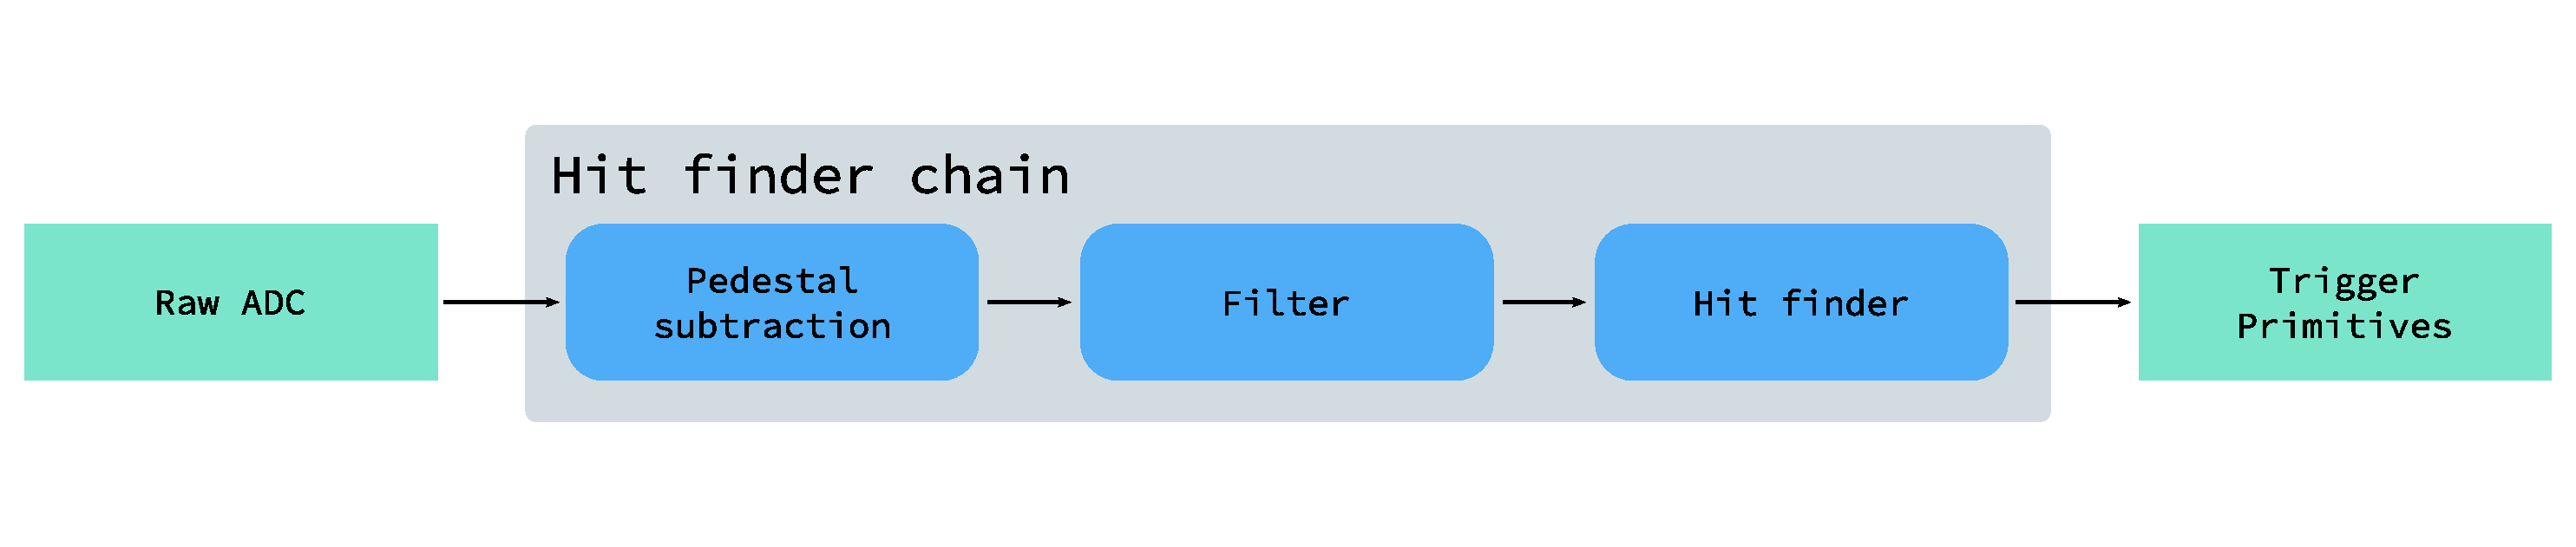
\includegraphics[width=0.99\linewidth]{Images/Matched_Filter/trigger_primitive_chain.pdf}
	\caption{Schematic representation of the Trigger Primitive Generation chain in the DUNE FD.}
	\label{fig:tpg_chain}
\end{figure}

This is particularly important for the induction planes. In general, signal peaks in the induction channels have smaller amplitude than the ones in the collection plane. This, together with the fact that the pulse shapes are bipolar, reduces our capacity to detect the hits on these channels. The inefficiency of detecting TPs in the induction planes (denoted as U and V planes) leads trigger algorithms to focus mainly on the TPs from the collection plane (so-called X plane). As a result, the possibility of making trigger decisions based on the coincidence of TPs across the three wire planes remains nowadays unexploited in DUNE. This will be beneficial for low energy events, as it adds redundancy to the algorithms, as well as for other physics that requires online directionality information, like the supernova pointing.

\begin{figure}[t]
	\centering
	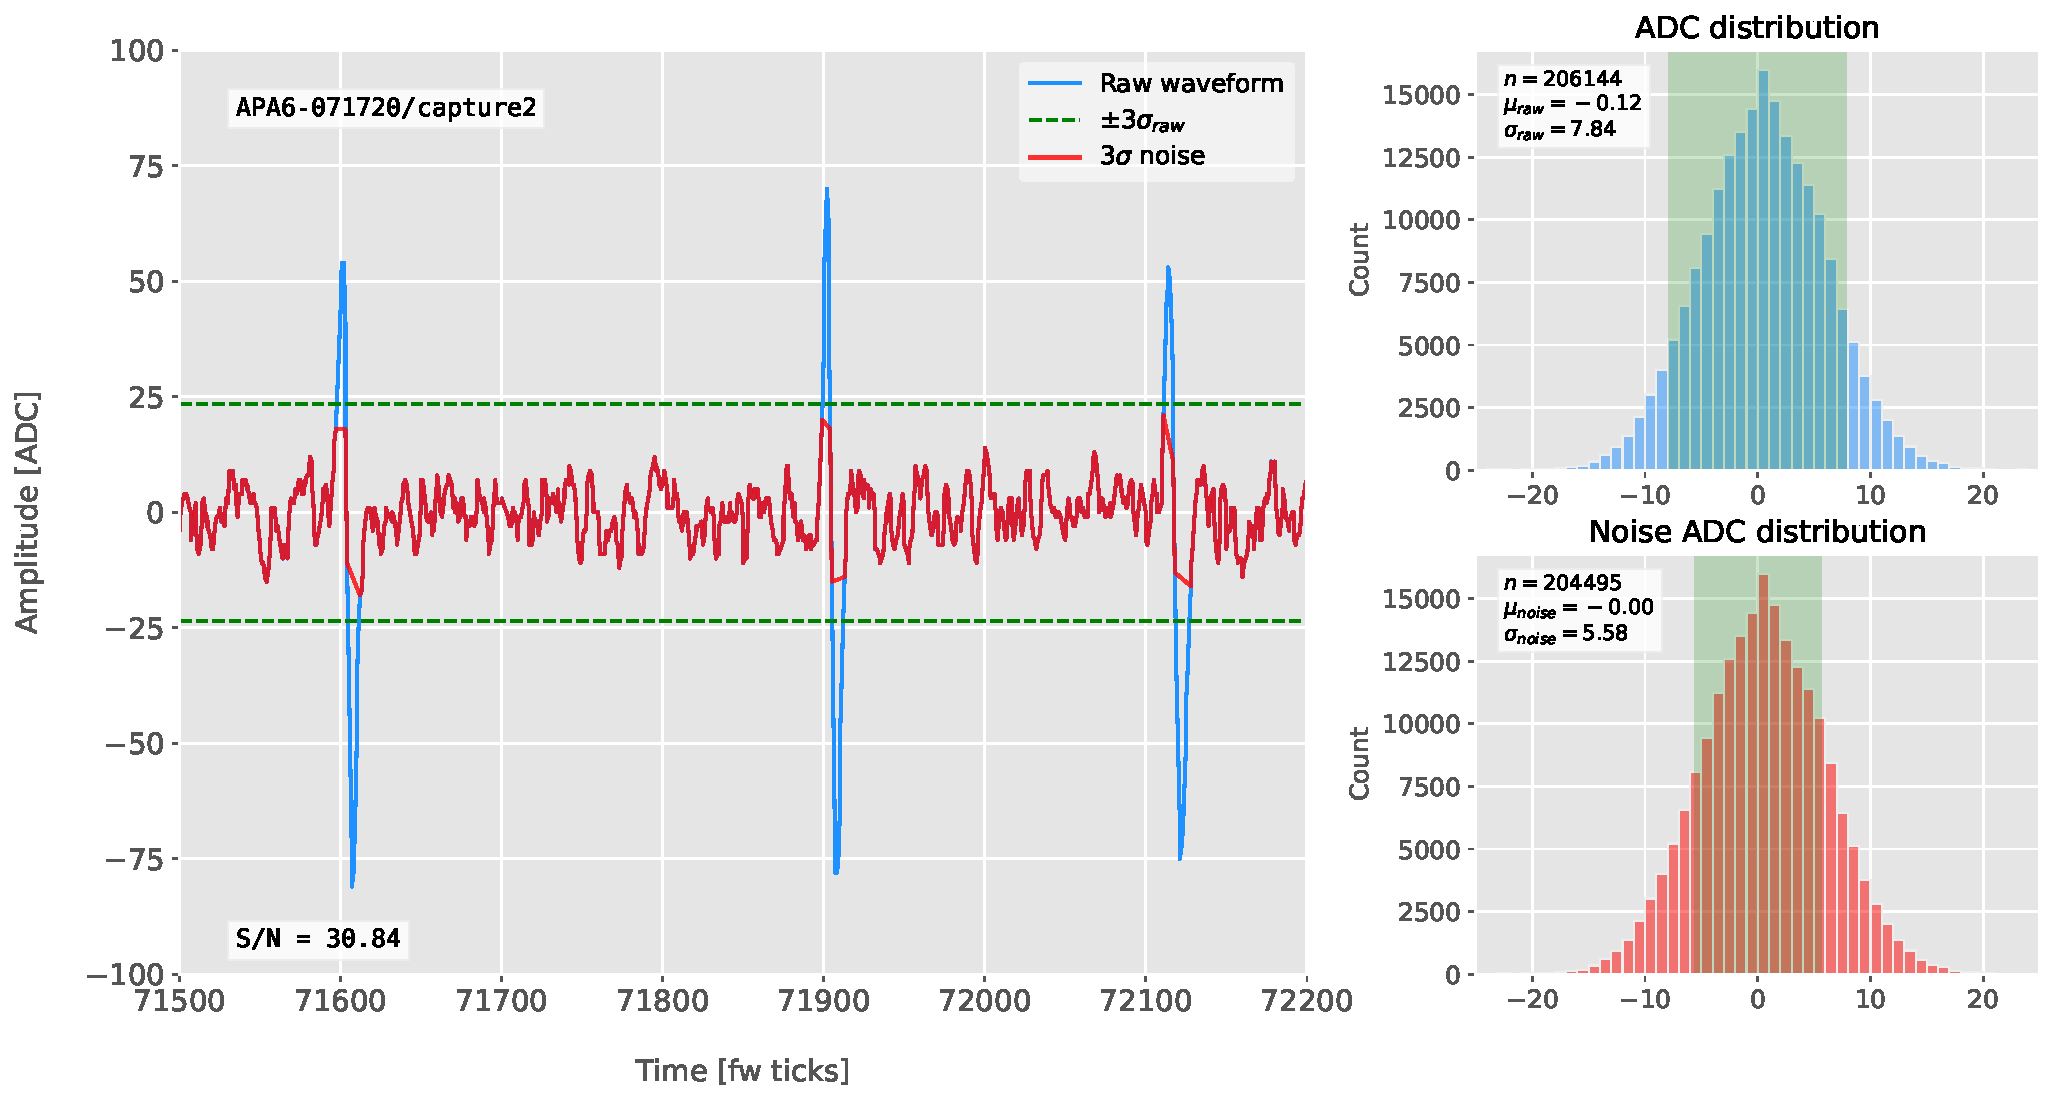
\includegraphics[width=1\linewidth]{Images/Matched_Filter/waveform_example_raw}
	\caption[Example unfiltered waveform from a ProtoDUNE-SP raw data capture.]{Left panel: Zoomed unfiltered waveform corresponding to channel $7840$ from the ProtoDUNE-SP raw data capture \texttt{felix-2020-07-17-21:31:44} (blue line). The green dashed lines mark the region $\pm3\sigma_{raw}$. The resulting noise waveform is also shown (red line). Top right panel: ADC distribution for channel $7840$, where the green shaded region represents $\pm \sigma_{raw}$. Bottom right panel: noise ADC distribution for channel $7840$, where the green shaded region represents $\pm \sigma_{noise}$.}
	\label{fig:adcs_nofir}
\end{figure}

A possible improvement of the current hit finder chain may require optimising the existing or choosing a new filter implementation. A filter strategy which benefits the induction signals may be able to enhance the detection efficiency of TPs from the induction planes and ideally make it comparable to that of the collection plane.  

The goal is to implement a better finite-impulse response filter and to evaluate its performance relative to the current filter. To do so, I need to take into account the limitations of the firmware: the FIR filter shall have maximum 32 coefficients (so-called taps) whose values are 12-bit unsigned integers. Although it is technically possible to include non-integer coefficients, it would be a technical challenge. For instance, in the HD design there are 40 FIR instances per APA, as there are 4 FIR blocks per optical link and 10 optical links per APA. Therefore, the impact of increasing the complexity of the filter will be amplified forty times in the FPGA load. With these restrictions, the task is to provide a set of 32 coefficients which yield an optimal filter performance for the induction channels. A solution compatible with the software hit finder implementation is not considered, due to its current limitations concerning the filtering stage.

\section{Signal-to-noise ratio definition}
\label{sec:matched_filter_sn_definition}

In the following, I use the signal to noise ratio (S/N) as a measure of the FIR filter performance. The S/N metrics allow us to compare different filter implementations and serve as a basis for more detailed studies presented later in this Chapter. Here, I demonstrate how to extract its value for a set of 
ProtoDUNE-SP data. Specifically, I use the ADC capture \texttt{felix-2020-07-17-21:31:44}, a raw data capture taken for firmware validation purposes. I define the S/N of a channel as the height of the signal peaks relative to the size of the noise. To quantify this, I first estimate the standard deviation of the ADC data for each channel, $\sigma_{\mathrm{ADC}}$. Then, I define the corresponding noise waveform to be the ADC values in the range $\pm 3~\sigma_{\mathrm{ADC}}$. From this new noise data I compute the mean and standard deviation, $\mu_{noise}$ and $\sigma_{noise}$, so I can write the S/N for any given channel as:
\begin{equation}
	\mathrm{S/N} = \frac{\max{[\mathrm{ADC}]} - \mu_{noise}}{\sigma_{noise}},
\end{equation}
where $\max{[\mathrm{ADC}]}$ is simply the maximum ADC value found in the corresponding channel.

\begin{figure}[t]
	\centering
	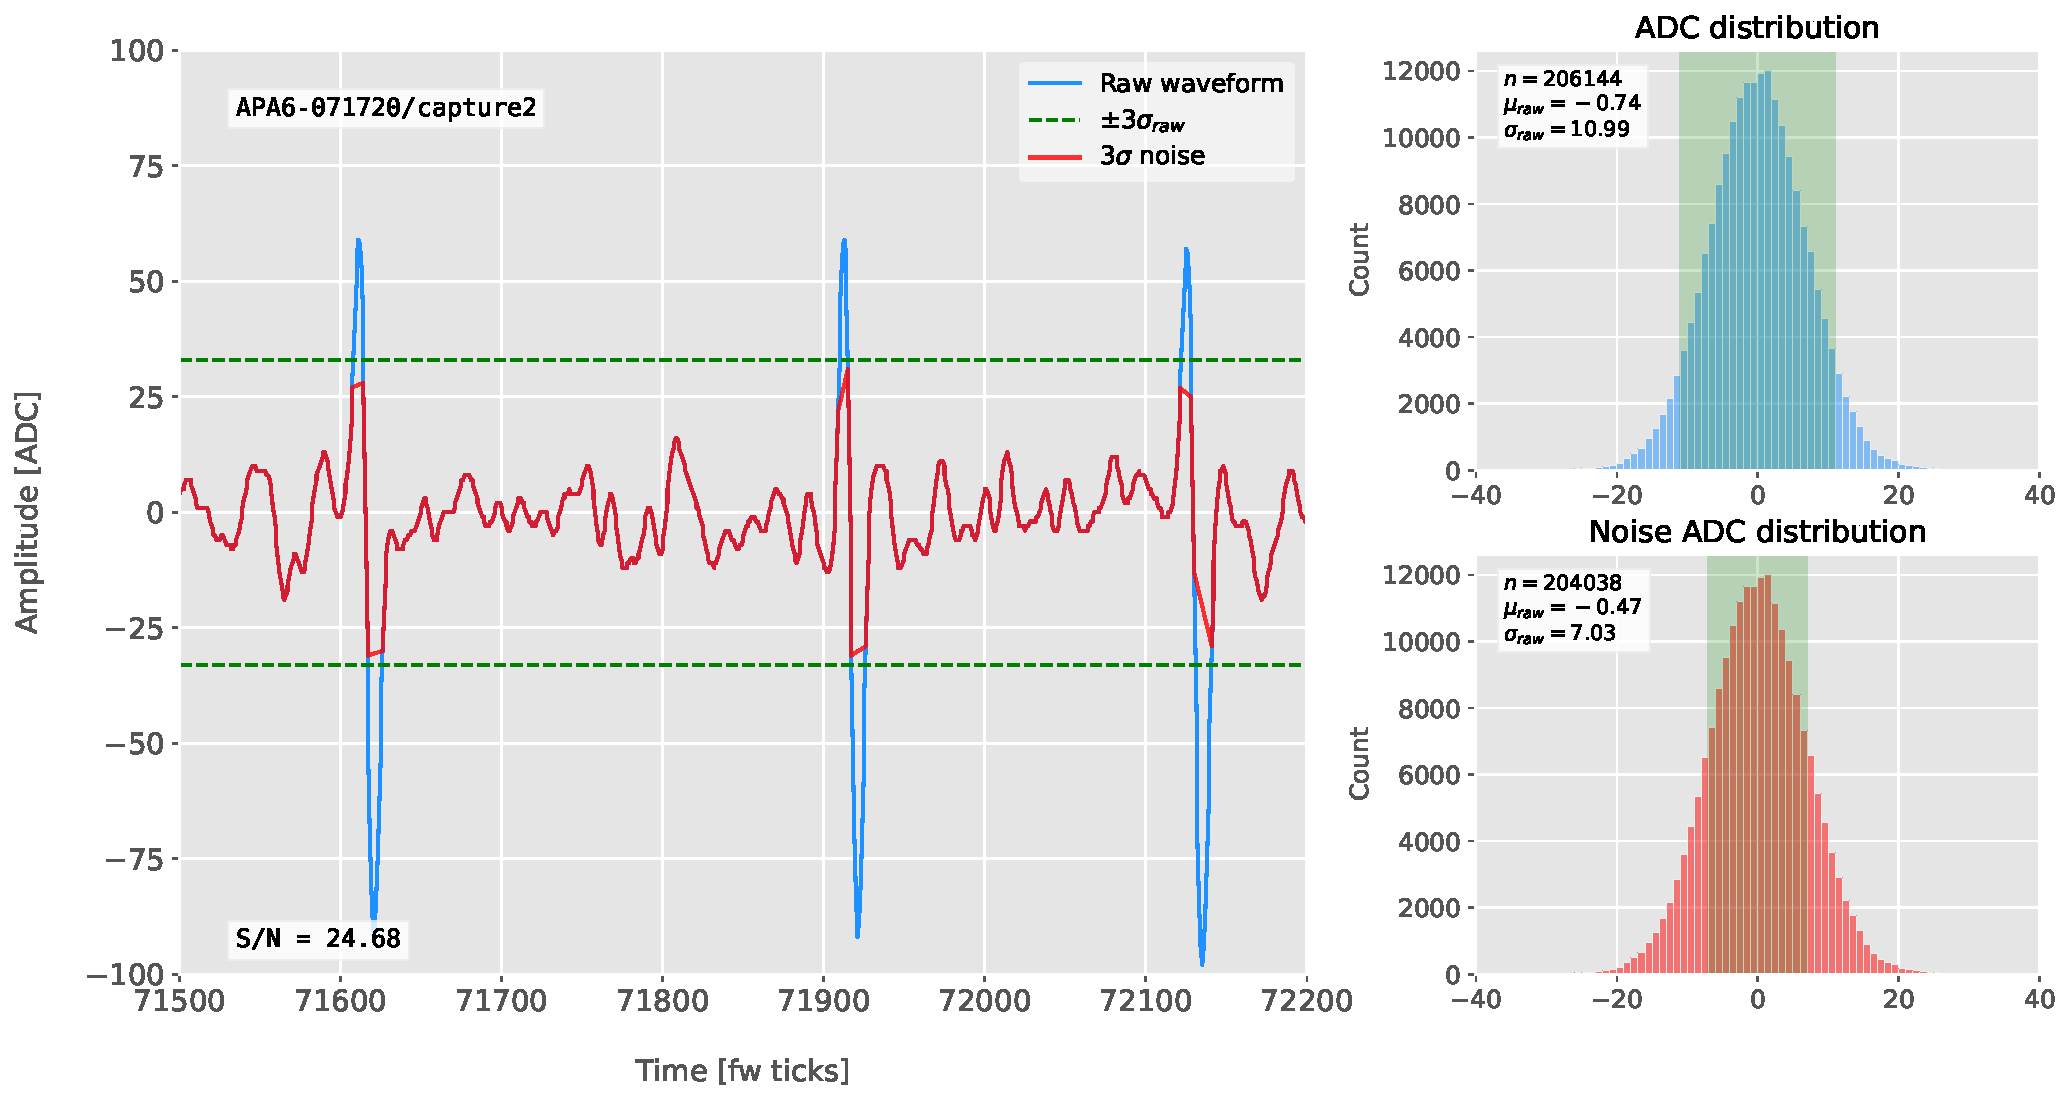
\includegraphics[width=1\linewidth]{Images/Matched_Filter/waveform_example_fir}
	\caption[Example filtered waveform from a ProtoDUNE-SP raw data capture.]{Left panel: Zoomed filtered waveform corresponding to channel $7840$ from the ProtoDUNE-SP raw data capture \texttt{felix-2020-07-17-21:31:44} (blue line). The filter used was the current implementation of the low-pass FIR filter in \texttt{dtp-firmware}. The green dashed lines mark the region $\pm3\sigma_{raw}$. The resulting noise waveform is also shown (red line). Top right panel: ADC distribution for channel $7840$ after filtering, where the green shaded region represents $\pm \sigma_{raw}$. Bottom right panel: noise ADC distribution for channel $7840$ after filtering, where the green shaded region represents $\pm \sigma_{noise}$.}
	\label{fig:adcs_fir}
\end{figure}

As an example, I apply this definition of the S/N to a waveform from one of the channels of the data capture. Figure \ref{fig:adcs_nofir} shows a zoomed region of the waveform corresponding to channel $7840$ (blue line), where one can clearly see three signal peaks and continuous additive noise\footnote{There are actually 6 peaks, 3 positive and 3 negative, but, because by design for induction channels the expected signal pulse shapes are bipolar, we treat them as a collection of 3 individual signals.}. I estimated the standard deviation of this raw waveform to be $\sigma_{raw} = 7.84 ~ \mathrm{ADC}$, and from this I am able to define the noise waveform (red line) as the ADC values in the range $\pm 23.52 ~ \mathrm{ADC}$. This way, I obtain $\mu_{noise} = 0.01 ~ \mathrm{ADC}$ and $\sigma_{noise} = 5.58 ~ \mathrm{ADC}$, which gives $\mathrm{S/N} = 30.84$.

I repeat this calculation now for the corresponding filtered waveform, using the current firmware FIR filter. Figure \ref{fig:adcs_fir} shows the same time window for the filtered waveform from channel $7840$ (blue line). In this case, the standard deviation of the waveform is larger than before, giving $\sigma_{raw} = 10.99 ~ \mathrm{ADC}$. The noise waveform (red line) is formed by selecting the ADC values in the $\pm 32.91 ~ \mathrm{ADC}$ range, which gives $\mu_{noise} = -0.47 ~ \mathrm{ADC}$ and $\sigma_{noise} = 7.03 ~ \mathrm{ADC}$. Finally, one obtains $\mathrm{S/N} = 24.68$. Notice that the value of S/N decreases after the filtering. Clearly, one can see that the noise baseline has increased by a factor of $1.35$ when we applied the FIR filter, and at the same time the amplitude of the signal peaks has remained almost unchanged, leading to this poorer S/N value.

\begin{comment}
\section{Low-pass FIR filter design}
\label{sec:matched_filter_fir}

To optimise the frequency response of a digital filter, we can use the Parks-McClellan algorithm, where one finds a set of $N$ real coefficients that give the best response for the specified pass-band and order of the filter \cite{McClellan2005}.

Taking the detector ticks as the time unit, the Nyquist frequency will simply be $1/2 \ \mathrm{ticks^{-1}}$. The current implementation of the filter seems to have as pass-band the range $[0,0.1] \ \mathrm{ticks^{-1}}$. This can be seen in Fig. \ref{fig:filter_comp}, where I show the power spectrum, in decibels, of that filter implementation (blue solid line). The Park-McClellan algorithm finds the optimal Chebyshev FIR filter \cite{Weinberg1960} taking as input the boundaries of the target pass-band and stop-band, which can be written in the form:
\begin{equation}
	\left\{ \begin{array}{c}
		\left[0, f_{c}\right] \\
		\left[ f_{c} + \delta f, f_{N}\right]
	\end{array} \right. ,
\end{equation}
where $f_{c}$ is the cut-off frequency, $\delta f$ is the transition width and $f_{N}$ is the aforementioned Nyquist frequency. A filter with a similar behaviour to the previous one can be obtained by setting $f_{c} = 0$ and $\delta f = 0.1 \ \mathrm{ticks}^{-1}$. The response of the resulting filter is also shown in Fig. \ref{fig:filter_comp} (blue solid line). Notice that the suppression of the stop-band is enhanced for this optimal filter. For comparison, I include the power response of the filter obtained by taking the integer part of the coefficients resulting from the Parks-McClellan method (red dashed line). One can see that it does not suppress that much the stop-band, in a similar way to the current implementation of the filter.

\begin{figure}[h!]
	\centering
	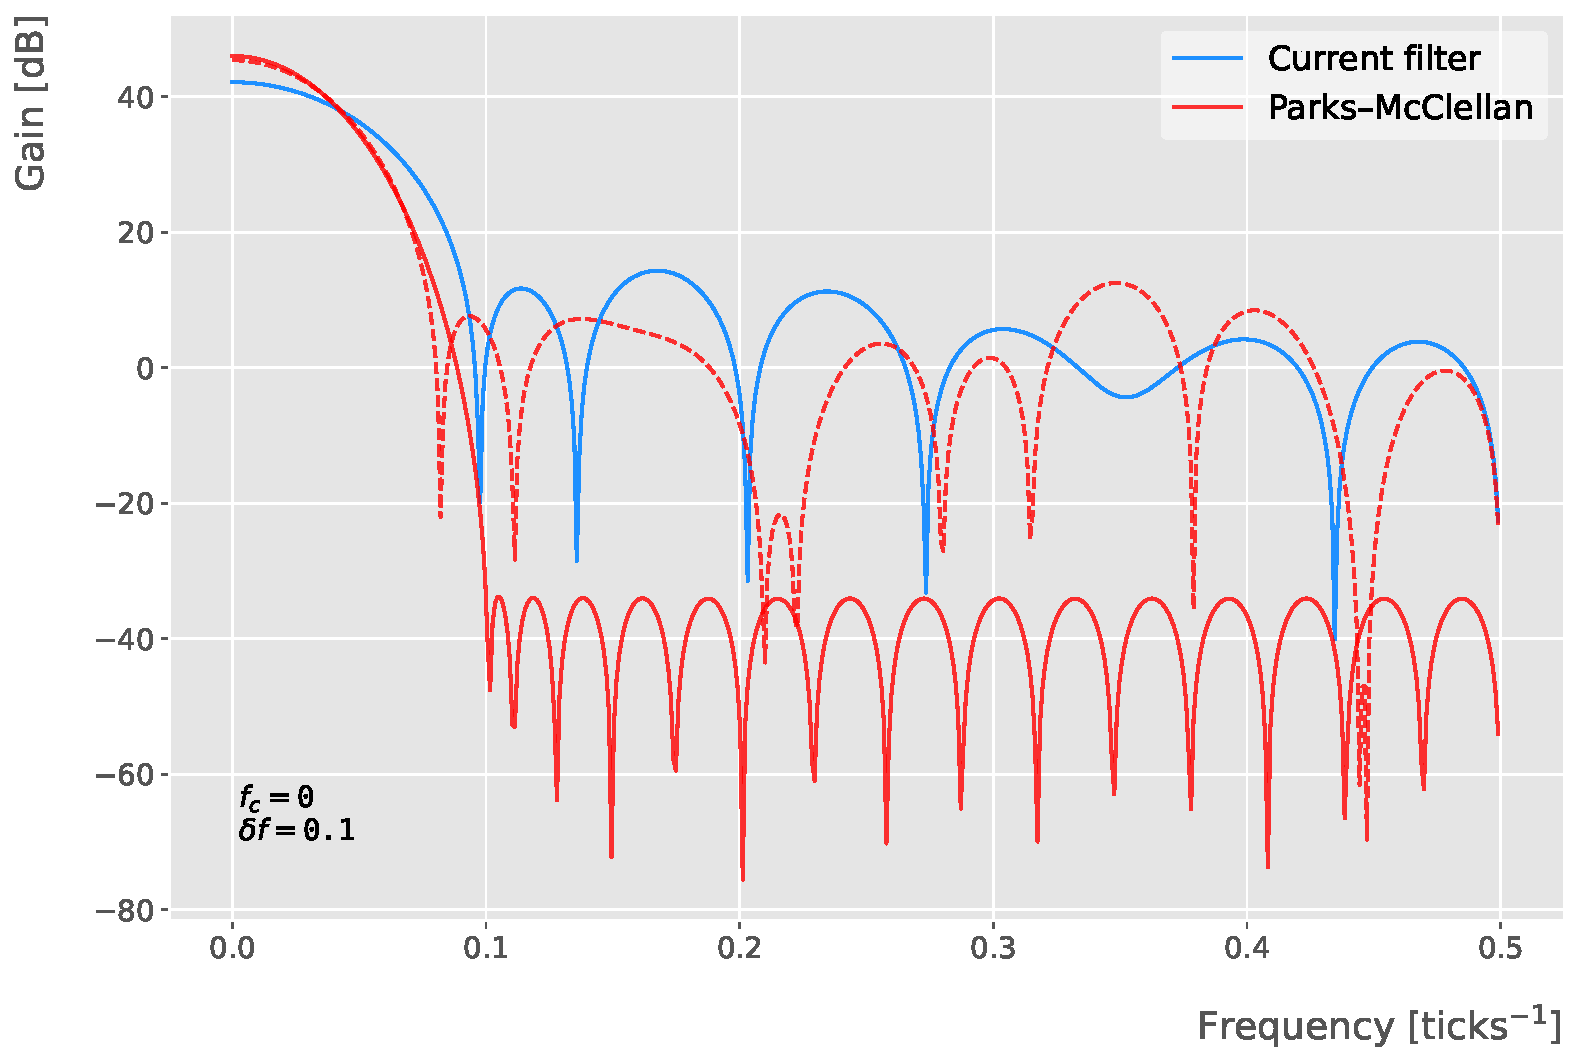
\includegraphics[width=0.8\linewidth]{Images/Matched_Filter/filter_comp}
	\caption[Power spectra for the current low-pass FIR filter and the optimal filter obtained using the Parks-McClellan algorithm.]{Power spectrum in decibels for the current implementation of the low-pass FIR filter in \texttt{dtp-firmware} (blue line), compared to the response of an optimal filter obtained using the Parks-McClellan algorithm for the same pass-band (red line). Also for comparison I include the spectrum of the optimal filter when taking only the integer part of the coefficients (red dashed line).}
	\label{fig:filter_comp}
\end{figure}

At this point, I tried to improve the performance of the FIR filter using the Park-McClellan method, i.e. maximise the overall S/N, using the available data captures. I did so by varying the values of the two quantities that parametrise the pass-band and stop-band, the cut-off frequency $f_{c}$ and the transition width $\delta f$.

\begin{figure}[t]
	\centering
	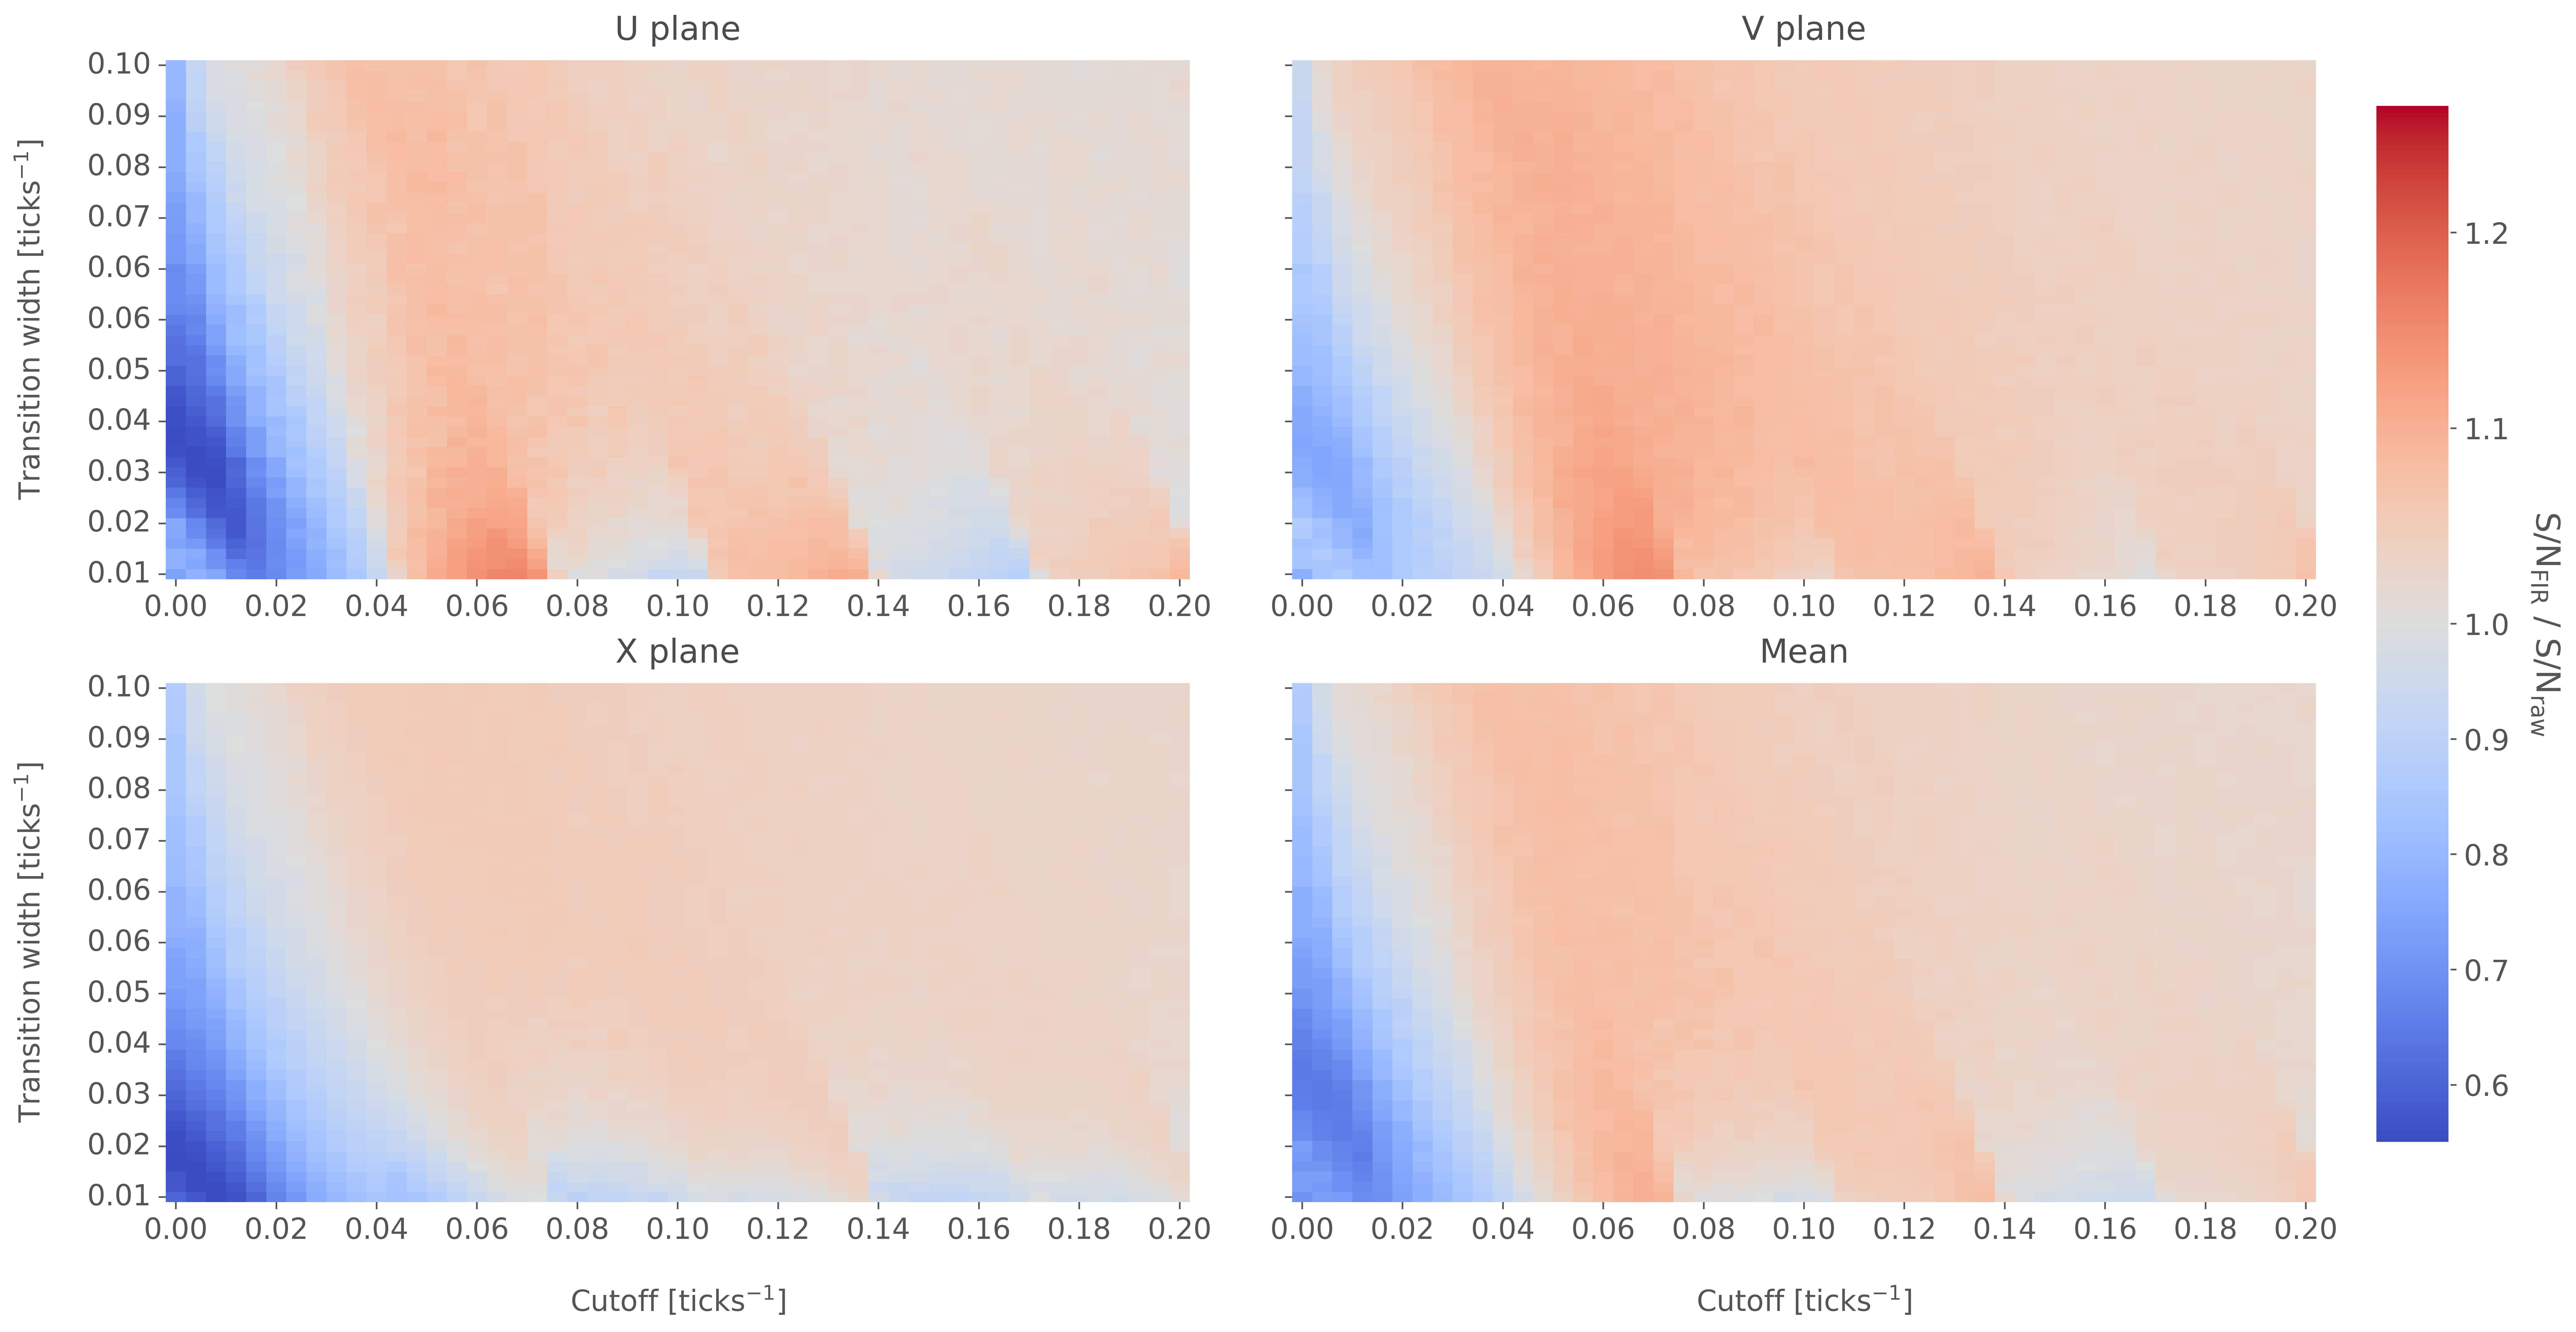
\includegraphics[width=1\linewidth]{Images/Matched_Filter/pm_fir_opt.png}
	\caption[Relative change in the S/N of the ProtoDUNE-SP raw data capture for different values of the cutoff frequency $f_{c}$ and the transition width $\delta f$.]{Relative change in the S/N for the ProtoDUNE-SP raw data capture \texttt{felix-2020-07-17-21:31:44}, using different values of the cutoff frequency $f_{c}$ and the transition width $\delta f$. The optimal Chebyshev filters were applied using just the integer part of the coefficients given by the Parks-McClellan algorithm.}
	\label{fig:fir_opt}
\end{figure}

\begin{figure}[t]
	\centering
	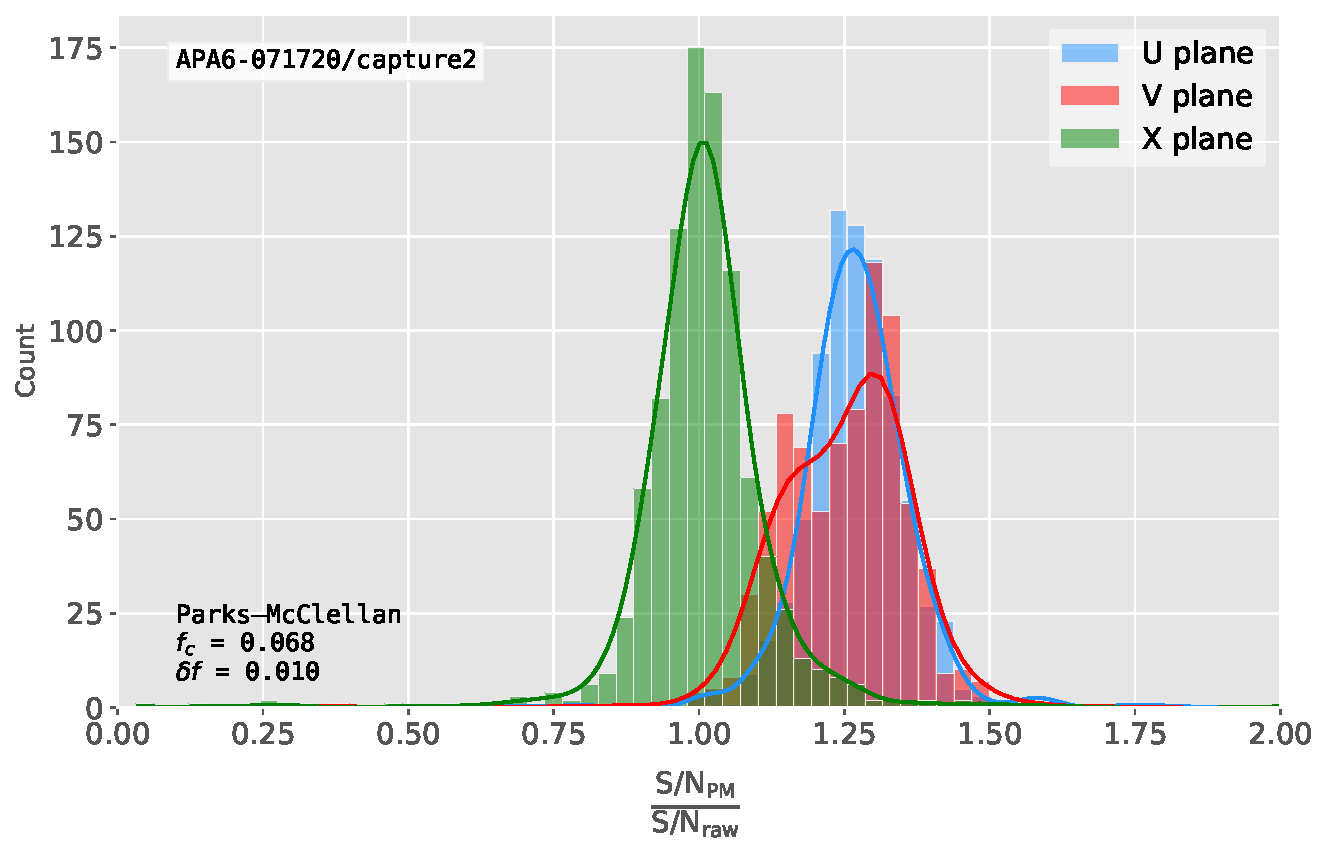
\includegraphics[width=0.85\linewidth]{Images/Matched_Filter/pm_fir_perf}
	\caption[Distribution of the relative change of the S/N on the different wire planes after the optimal FIR filter was applied.]{Distribution of the relative change of the S/N on the different wire planes from the ProtoDUNE-SP raw data capture \texttt{felix-2020-07-17-21:31:44} after the optimal Chebyshev filter was applied. The filter was computed with the Parks-McClellan algorithm using a cutoff of $f_{c} = 0.068 \ \mathrm{ticks}^{-1}$ and a transition width $\delta f = 0.010 \ \mathrm{ticks}^{-1}$.}
	\label{fig:fir_best}
\end{figure}

Figure \ref{fig:fir_opt} shows the average relative change in the S/N (i.e. the ratio between the value of the S/N after and before the filtering) for capture \texttt{felix-2020-07-17-21:31:44}, when using filters designed with the Parks-McClellan algorithm for the specified values of the cut-off frequency $f_{c}$ and the transition width $\delta f$, restricted to integer values for the filter coefficients. One can clearly distinguish different regions where we get an improvement of up to a factor of $1.35$ for the U plane. For large values of $f_{c} + \delta f$ the ratio tends to $1$, as expected. In that limit the width of the stop-band goes to $0$, meaning that no frequencies are filtered out and thus the waveform remains the same.

As it can be seen in Fig. \ref{fig:fir_opt} (bottom right panel) the configuration which gives the best mean performance for the three planes is $f_{c} = 0.068 \ \mathrm{ticks}^{-1}$ and $\delta f = 0.010 \ \mathrm{ticks}^{-1}$. We can use these to see how the filter affects the different channels. Figure \ref{fig:fir_best} shows the distribution of the S/N improvement values for all the channels in the raw ADC capture \texttt{felix-2020-07-17-21:31:44}, separated by wire plane, after the optimal Chebyshev filter was applied. One can see that there is a clear improvement for both U and V induction planes, obtaining a mean change of $1.25$ and $1.30$ for them, respectively. However, in the case of the X collection plane the distribution peaks around $1$, meaning that an important fraction of channels in that plane get a slightly worse S/N after the filter is applied. This is not a big issue, as the S/N for collection channels is usually much higher than the one for induction channels.

The results I obtained optimising the low pass filter with the Parks-McClellan method are promising. Nonetheless, the improvement found is rather marginal. Thus, I explored alternative approaches to the filtering problem, which may yield better outputs. This way, I found a possible solution in matched filters. By construction, this kind of filters offer the best improvement on the S/N.
\end{comment}

\section{Matched filters}
\label{sec:matched_filter_matched_filter}

In the context of signal processing, a matched filter is the optimal linear filter for maximising the S/N in the presence of additive noise. It is obtained by convolving a conjugated time-reversed known template with an unknown signal to detect the presence of the template in the signal \cite{Turin1960}.

\begin{figure}[t]
	\centering
	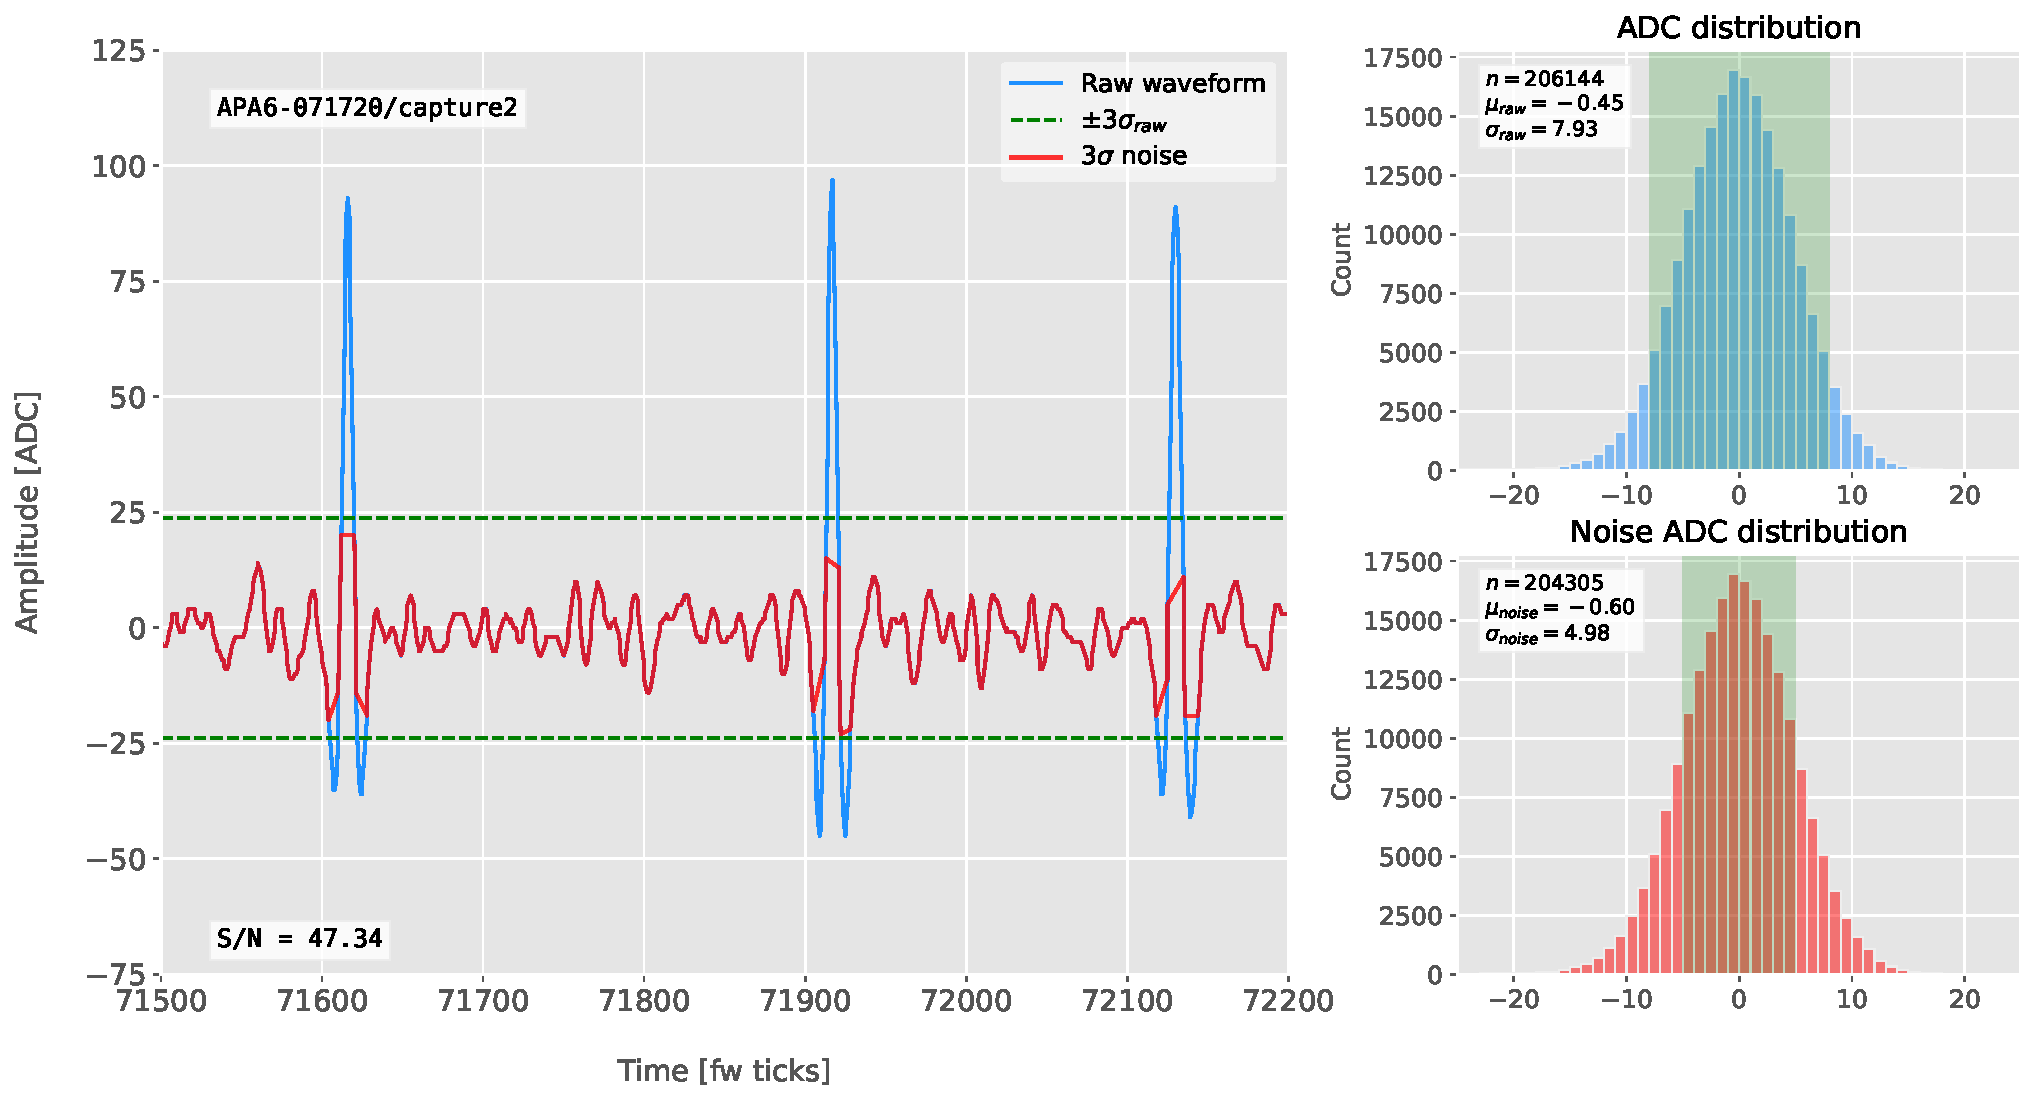
\includegraphics[width=1\linewidth]{Images/Matched_Filter/waveform_example_mf}
	\caption[Example matched filtered waveform from a ProtoDUNE-SP raw data capture.]{Left panel: Zoomed match filtered waveform corresponding to channel $7840$ from the ProtoDUNE-SP raw data capture \texttt{felix-2020-07-17-21:31:44} (blue line). The filter used was directly extracted from the data, being the $32$ values around the first peak in the original waveform. The green dashed lines mark the region $\pm3\sigma_{raw}$. The resulting noise waveform is also shown (red line). Top right panel: ADC distribution for channel $7840$ after match filtering, where the green shaded region represents $\pm \sigma_{raw}$. Bottom right panel: noise ADC distribution for channel $7840$ after match filtering, where the green shaded region represents $\pm \sigma_{noise}$}
	\label{fig:adcs_mf}
\end{figure}

For a discrete signal, assuming that the additive noise is Gaussian, the impulse-response vector associated to the matched filter is given by:
\begin{equation}
	h \propto s,
\end{equation}
where $s$ is a reversed signal template sequence of length $N$ equal to the order of the filter. A detailed discussion on the derivation of this formula can be found in App. \ref{sec:matched_filter_impulse}.

\begin{comment}
Given a known signal sequence $s(t)$ and another (a priori unknown) noise sequence $n(t)$, the input signal can be written as:
\begin{equation}\label{2.4.1}
	x(t) = s(t) + n(t).
\end{equation}

Now, considering a linear time-invariant filter, whose impulse-response function I will refer to as $h(t)$, one can write the output signal as:
\begin{equation}\label{2.4.2}
	\begin{split}
		y(t) &= x(t)*h(t)\\
		&= \left(s(t) + n(t)\right)*h(t)\\
		&= y_{s}(t) + y_{n}(t),
	\end{split}
\end{equation}
where $y_{s}(t)$ and $y_{n}(t)$ are simply the outputs of the filter due to the signal and the noise components respectively.

The goal of the matched filter is to detect the presence of the signal $s(t)$ in the input sample $x(t)$ at a certain time $t_{0}$, which effectively means that we need to maximise the S/N at that given time. This way, what one wants is to have a filter which gives a much bigger output when the known signal is present than when it is not. Putting it in other words, the instantaneous power of the signal output $y_{s}(t)$ should be much larger than the average power of the noise output $y_{n}(t)$ at some time $t_{0}$.

For the case of the filtered signal, one can easily re-write it as an inverse Fourier transform:
\begin{equation}\label{2.4.3}
	y_{s}(t) = \frac{1}{2\pi} \int_{-\infty}^{\infty} \mathrm{d}\omega \ H(\omega) S(\omega) \mathrm{e}^{i \omega t},
\end{equation}
where $H(\omega)$ and $S(\omega)$ are the Fourier transforms of the impulse-response function (i.e. the transfer function of the filter) and of the input signal, respectively.

Now, focusing on the noise part, we can use the Wiener-Khinchin theorem \cite{Goodman1985} to write the mean power of the noise after filtering as:
\begin{equation}\label{2.4.4}
	E|y_{n}(t)|^{2} = \frac{1}{2\pi} \int_{-\infty}^{\infty} \mathrm{d}\omega \ |H(\omega)|^{2} S_{n}(\omega),
\end{equation}
where $S_{n}(\omega)$ is the power spectral density of the noise.

Having these, one can write the instantaneous S/N at time $t_{0}$ as:
\begin{equation}\label{2.4.5}
	\begin{split}
		\left(\frac{S}{N}\right)_{t_{0}} &= \frac{|y_{s}|^{2}}{E|y_{n}(t)|^{2}}\\
		&= \frac{1}{2\pi} \frac{\left|\int_{-\infty}^{\infty} \mathrm{d}\omega \ H(\omega) S(\omega) \mathrm{e}^{i \omega t_{0}}\right|^{2}}{\int_{-\infty}^{\infty} \mathrm{d}\omega \left|H(\omega)\right|^{2} S_{n}(\omega)}.
	\end{split}
\end{equation}

Once we have this expression, we need to find its upper limit to determine what would be the optimal choice for the transfer function. For this, we use the Cauchy-Schwarz inequality, which in the present case takes the form:
\begin{equation}\label{2.4.6}
	\left|\int_{-\infty}^{\infty} \mathrm{d}x \ f(x) g(x)\right|^{2} \leq \int_{-\infty}^{\infty} \mathrm{d}x \ \left|f(x)\right|^{2} + \int_{-\infty}^{\infty} \mathrm{d}x \ \left|g(x)\right|^{2},
\end{equation}
for any two analytical functions $f(x)$ and $g(x)$. One can prove that making the choice:
\begin{equation}\label{2.4.7}
	\begin{split}
		&f(x) = H(\omega) \sqrt{S_{n}(\omega)}\mathrm{e}^{i \omega t_{0}},\\
		&g(x) = \frac{S(\omega)}{\sqrt{S_{n}(\omega)}},
	\end{split}
\end{equation}
leads to the following upper bound for the S/N:
\begin{equation}\label{2.4.8}
	\left(\frac{S}{N}\right)_{t_{0}} \leq \frac{1}{2\pi}\int_{-\infty}^{\infty} \mathrm{d}\omega \  \frac{\left|S(\omega)\right|^{2}}{S_{n}(\omega)}.
\end{equation}

From Eqs. (\ref{2.4.5}), (\ref{2.4.6}) and (\ref{2.4.7}) one can also derive the form of the transfer function such that the upper bound is exactly reached \cite{Dwork1950}:
\begin{equation}\label{2.4.9}
	H(\omega) \propto \frac{S^{*}(\omega) \mathrm{e}^{-i \omega t_{0}}}{S_{n}(\omega)}.
\end{equation}

From this last expression we can clearly see the way the matched filter acts. As the transfer function is proportional to the Fourier transform of the signal it will try to only pick the frequencies present in the signal \cite{Wainstein1962}.

The matched filter transfer function can be greatly simplified if the input noise is Gaussian. In that case, the power spectral density of the noise is a constant, so it can be re-absorbed in the overall normalisation of the transfer function. Moreover, considering that the input signal is a real function, one can simply set $S^{*}(\omega) = S(-\omega)$, which gives:
\begin{equation}\label{2.4.10}
	H(\omega) \propto S(-\omega) \mathrm{e}^{-i \omega t_{0}}.
\end{equation}

For a discrete signal, one can think of the input and impulse-response sequences as vectors. Then, the matched filter tries to maximise the inner product of the signal and the filter while minimising the output due to the noise by choosing a filter vector orthogonal to the latter. In the case of additive noise, that leads to the impulse-response vector:
\begin{equation}\label{2.4.11}
	h = \frac{1}{\sqrt{s^{\dagger} R_{n}^{-1} s}} \ R_{n}^{-1} s,
\end{equation}
where $s$ is a reversed signal template sequence of length $N$ equal to the order of the filter and $R_{n}$ is the covariance matrix associated with the noise sequence $n$. For the Gaussian noise case, the covariance matrix is simply the unit matrix, so the above expression simplifies again to:
\begin{equation}\label{2.4.12}
	h = \frac{s}{|s|}.
\end{equation}
\end{comment}

To test whether this choice of filter is appropriate one needs to choose a signal template. As an example of how a matched filter would affect our signal, I simply took the matched filter coefficients to be the 32 ADC values around a signal peak present in the data. In Fig. \ref{fig:adcs_mf} (left panel) I plotted a zoomed region for channel $7840$ in the raw data capture \texttt{felix-2020-07-17-21:31:44}, after applying the matched filter described before (blue line). When compared to the raw and FIR filtered case (see Figs. \ref{fig:adcs_nofir} and \ref{fig:adcs_fir}), after applying the matched filter the standard deviation of the noise waveform (red line) decreases and at the same time the signal peaks are enhanced. This leads to an improvement of the S/N by a factor of $1.92$ when compared to the raw waveform.

To obtain the matched filter that is more suitable for our data, I explored different configurations of signal templates. I parametrised the signal using the bipolar function:
\begin{equation}\label{2.4.13}
	f(x) = -A (x + \delta) \ \mathrm{e}^{-x^{2}/\sigma^{2}},
\end{equation}
where the parameter $\delta$ controls the asymmetry between the positive and negative peaks and $\sigma$ controls their width. The amplitude parameter $A$ is set such that it keeps the height of the biggest peak to be less than $200$ ADC in absolute value.

\begin{figure}[t]
	\centering
	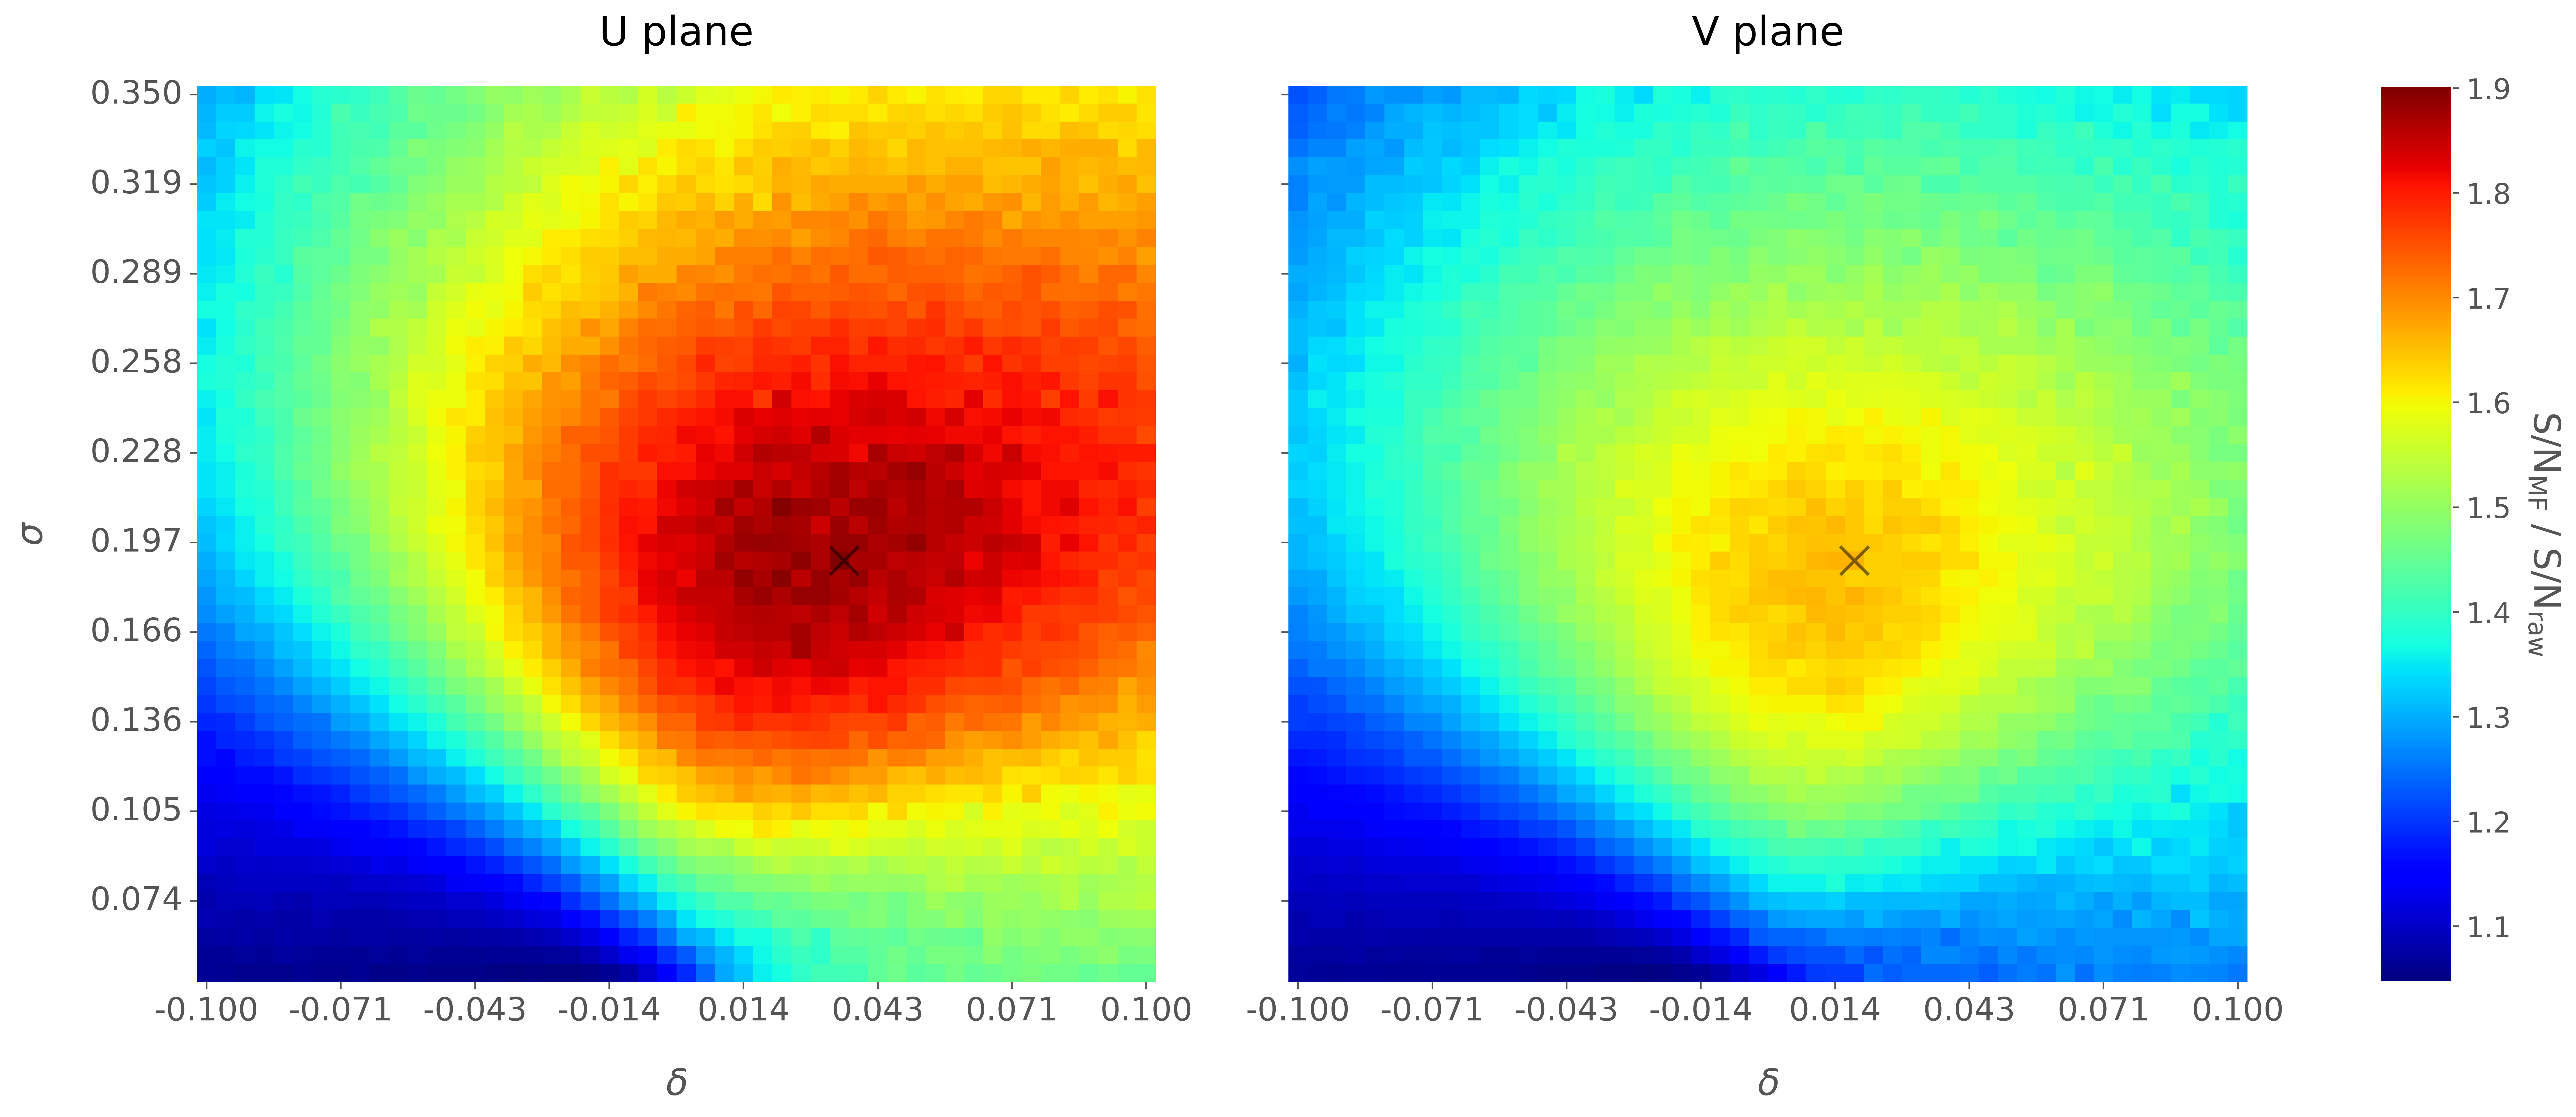
\includegraphics[width=1\linewidth]{Images/Matched_Filter/mf_fir_opt.png}
	\caption[Relative change in the S/N for the ProtoDUNE-SP raw data capture for different values of $\delta$ and $\sigma$ from the matched filter parametrisation.]{Relative change in the S/N for the ProtoDUNE-SP raw data capture \texttt{felix-2020-07-17-21:31:44} for different values of $\delta$ and $\sigma$ from the matched filter parametrisation in Eq. (\ref{2.4.13}). The black crosses in both panels denote the location of the maximum ratio value.}
	\label{fig:mf_opt}
\end{figure}

As this parametrisation is only adequate for bipolar signals I will focus exclusively on the induction channels. Also, to achieve the best possible performance, I optimise the coefficients for the U and V planes separately. However, as I will discuss, the differences are not very pronounced. In case it is not technically possible to separate channels in the firmware according to the plane they are coming from and use different sets of filter coefficients for them, we can just find a common set of coefficients. In such case, I do not expect the results to change drastically.

Figure \ref{fig:mf_opt} presents the results of the parameter scan, for channels in the induction planes U (left panel) and V (right panel). For each configuration of $\sigma$ and $\delta$ the resulting matched filter was applied to all channels in the corresponding plane within the data capture \texttt{felix-2020-07-17-21:31:44}. The change in S/N is computed with respect to the raw waveforms, and then the mean value for all channels is kept as a score for each filter. One can see that the improvements obtained for the U plane are in general higher than the ones for the V plane. However, these ratios are substantially higher than the ones obtained for the low-pass FIR filters. For the optimal configurations, I attained improvements up to a factor of $1.85$ for the U plane and $1.65$ for the V plane.

The sets of optimal matched filter coefficients were obtained for the parameters $\delta = 0.035$, $\sigma = 0.191$ for the U plane and $\delta = 0.018$, $\sigma = 0.191$ for the V plane. I show these two sets of coefficients in Fig. \ref{fig:mf_perf} (left panel). Figure \ref{fig:mf_perf} (right panel) shows the distribution of the S/N improvement after the optimal match filters for the U and V were applied to the corresponding channels in the raw data capture \texttt{felix-2020-07-17-21:31:44}. As mentioned before, the mean improvement achieved for the U plane channels is slightly higher than the one for the V channels. Note, however, that the spread of the distribution for the V plane is smaller than the one for the U plane.

Overall, one can see that the improvements on the S/N are much more significant in the case of the matched filter than they were for the low-pass FIR filters, described in App. \ref{sec:matched_filter_fir}. The analysis of the raw data captures from ProtoDUNE-SP suggests that matched filters increase the S/N of induction channels by a factor of $1.5$ more than the optimal low-pass FIR filters.

Although these results are by themselves great points in favour of the matched filter, more studies are needed to completely assess the robustness of this approach. I proceeded then to test the matched filter with simulated data samples.

\begin{figure}[t]
	\begin{subfigure}{0.5\textwidth}
		\centering
		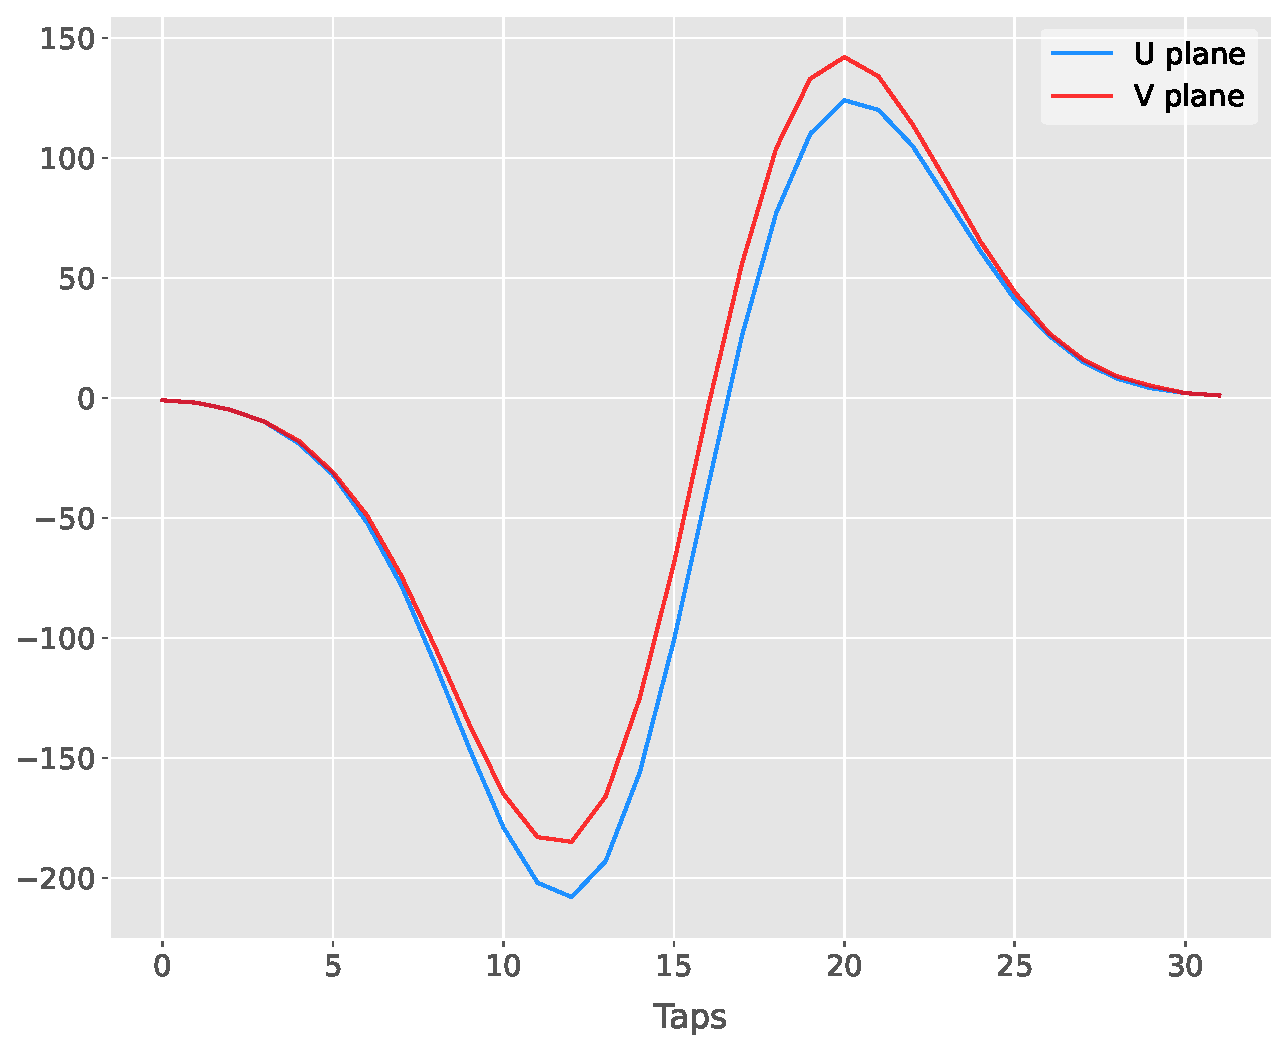
\includegraphics[width=.99\linewidth]{Images/Matched_Filter/optimal_coeffs}
	\end{subfigure}
	\begin{subfigure}{0.5\textwidth}
		\centering
		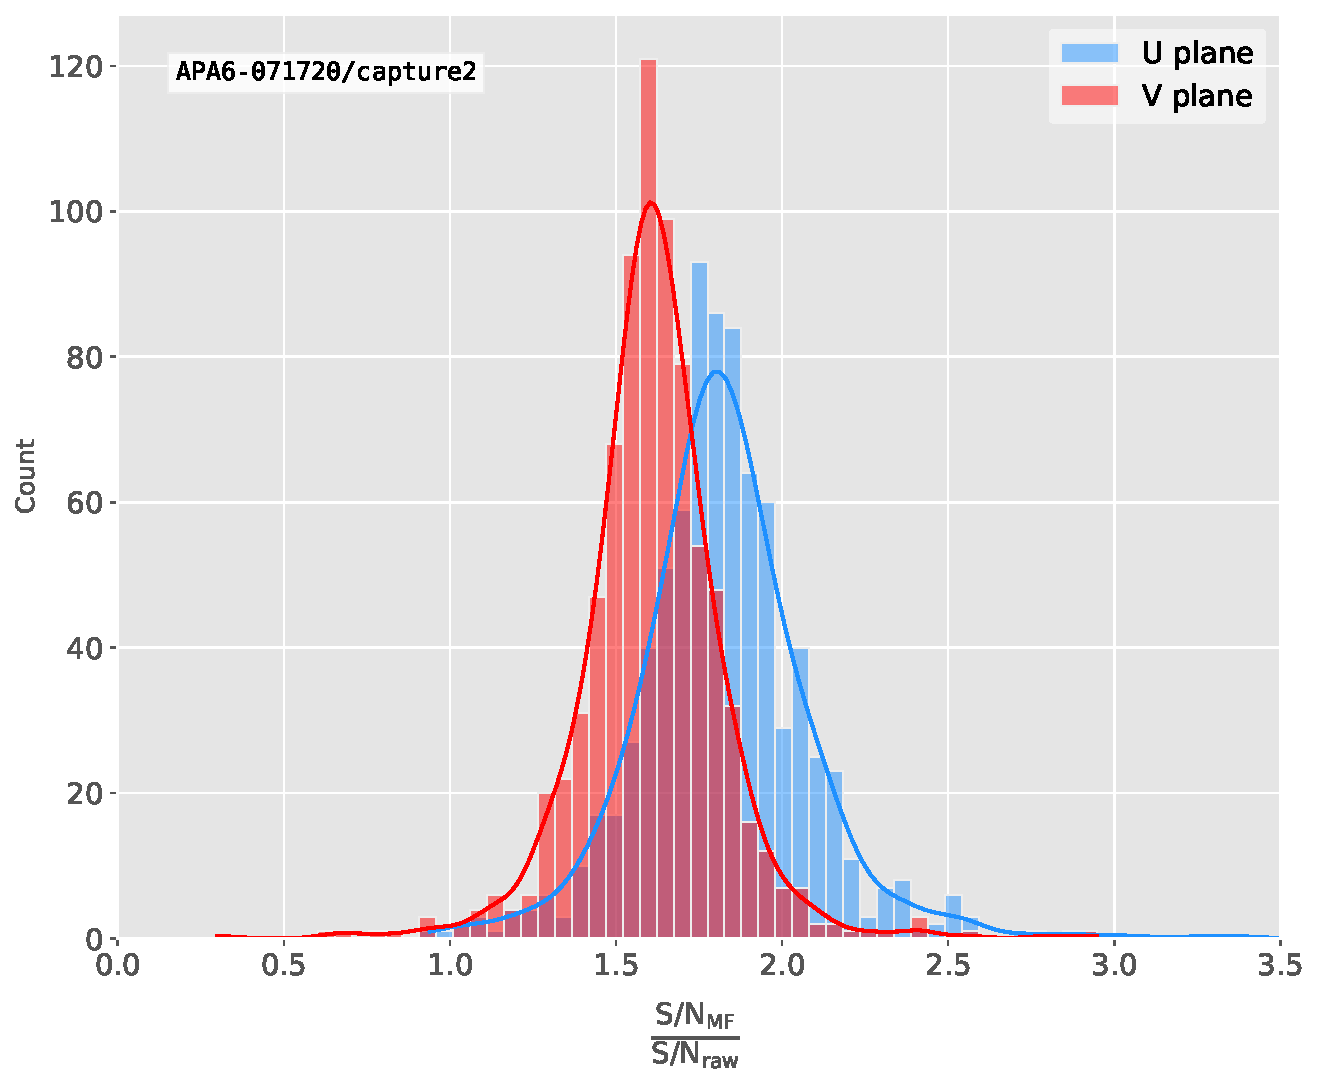
\includegraphics[width=.99\linewidth]{Images/Matched_Filter/improvement_capture}
	\end{subfigure}
	\caption[Distribution of the relative change of the S/N on the induction planes from the ProtoDUNE-SP raw data capture after their respective optimal matched filters were applied.]{Left panel: Optimal matched filter coefficients for the U (blue line) and V (red line) planes. The filters were computed with our parametrisation in Eq. (\ref{2.4.13}) for the parameter values $\delta = 0.035$, $\sigma = 0.191$ and $\delta = 0.018$, $\sigma = 0.191$ respectively. Right panel: Distribution of the relative change of the S/N on the two induction wire planes from the ProtoDUNE-SP raw data capture \texttt{felix-2020-07-17-21:31:44} after their respective optimal matched filters were applied.}
	\label{fig:mf_perf}
\end{figure}

\section{Monte Carlo studies}
\label{sec:matched_filter_mc_studies}

To further test the matched filter, the next step is to generate and process data samples using LArSoft \cite{Church2013}, the simulation and reconstruction software of the DUNE FD. In this way, one can control the particle content of the samples, the orientation of the tracks and their energy, and therefore see how the matched filter behaves in various situations.

To begin with, I prepared different monoenergetic and isotropic samples containing a single particle per event. Each sample contains a different particle species, namely electrons, muons, protons and neutral pions, all with a kinetic energy of $E_{k} = 100 \ \mathrm{MeV}$. I chose these because of the fairly different topologies they generate in the liquid argon, ranging from shower-like to track-like.

The event were generated with the single particle gun, and the Geant4 stage of the LArSoft simulation \cite{Church2013} was performed with the standard configuration for the DUNE FD HD design.

\begin{figure}[t]
	\begin{subfigure}{0.5\textwidth}
		\centering
		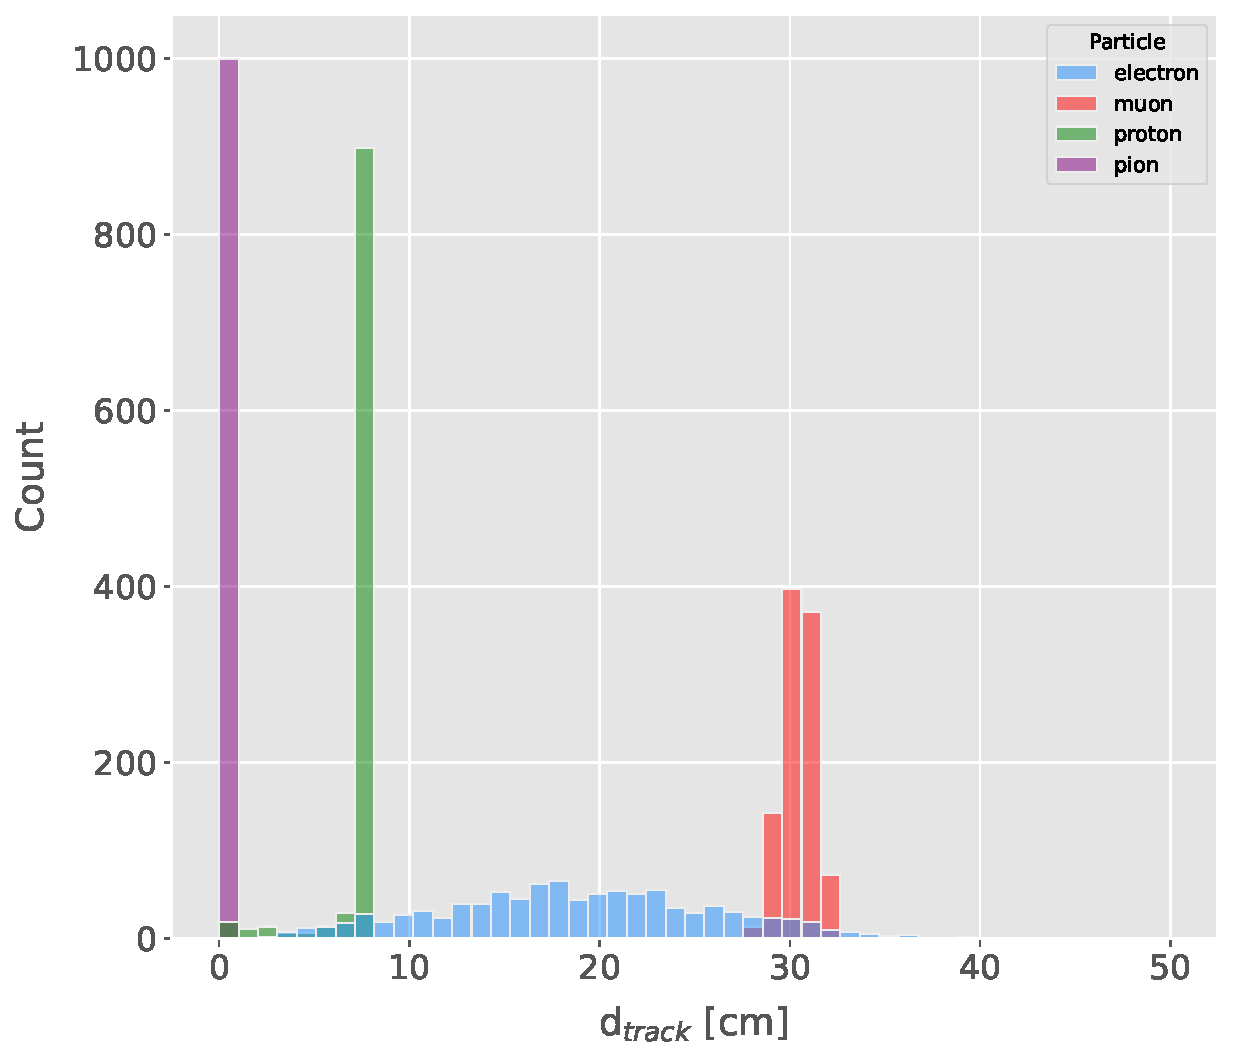
\includegraphics[width=.99\linewidth]{Images/Matched_Filter/particle_length}
	\end{subfigure}
	\begin{subfigure}{0.5\textwidth}
		\centering
		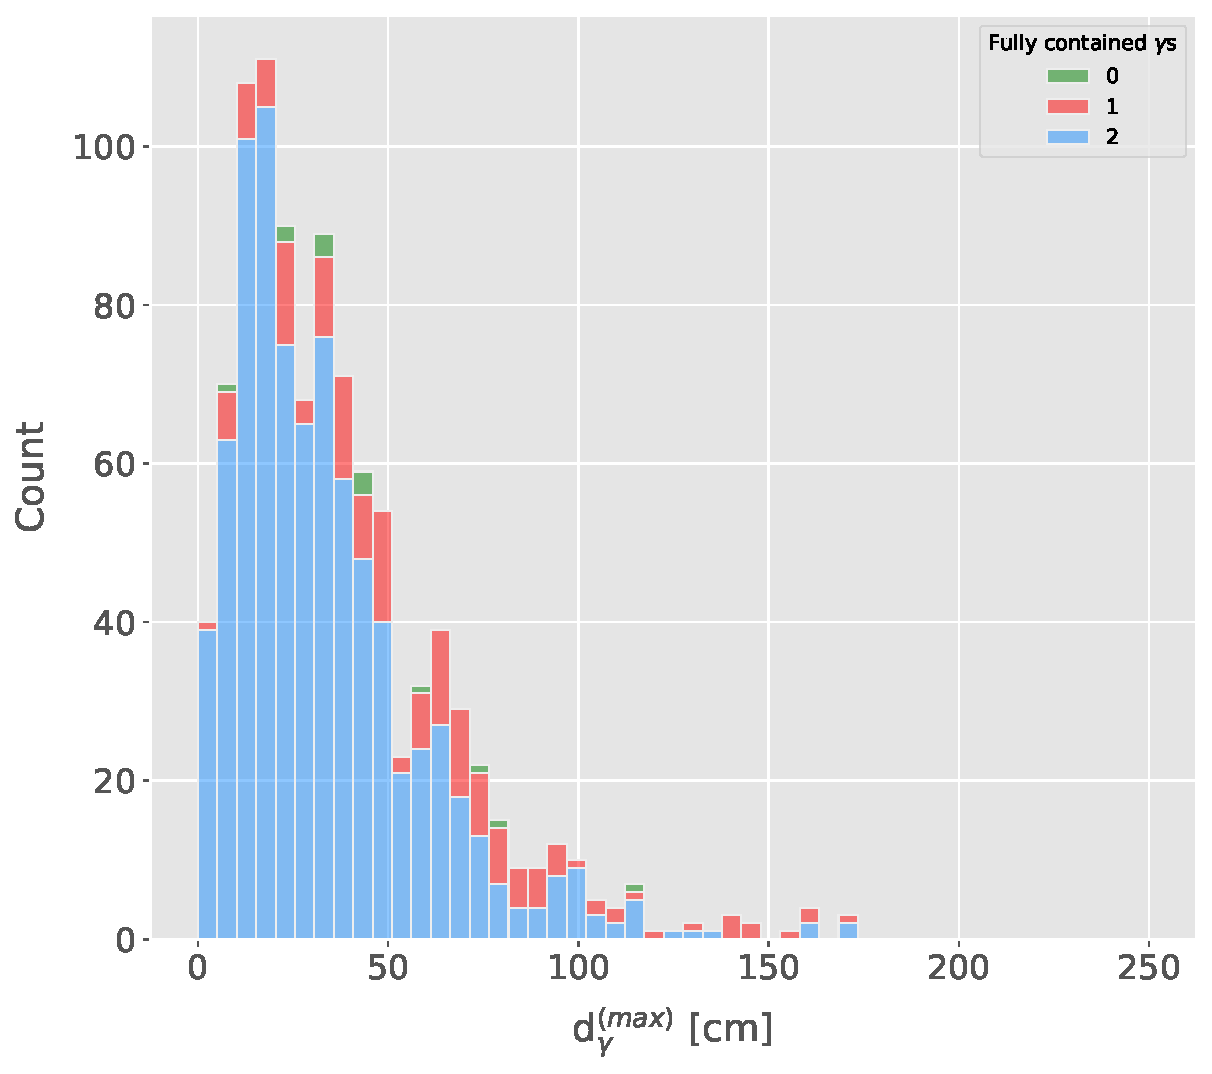
\includegraphics[width=.99\linewidth]{Images/Matched_Filter/gamma_length}
	\end{subfigure}
	\caption[Distributions of the particles track length in the liquid argon for the generated single particle monoenergetic samples.]{Left panel: distributions of the particles track length in the liquid argon for the generated $E_{k} = 100 \ \mathrm{MeV}$ monoenergetic samples, electrons (blue), muons (red), protons (green) and neutral pions (purple). Right panel: distribution of the length of the longest photon in the neutral pion sample after the decay process $\pi^{0} \rightarrow \gamma\gamma$.}
	\label{fig:lengths}
\end{figure}

For simplicity, I restricted the particles to start drifting in a single TPC volume\footnote{A TPC volume is defined as the drift region between a single APA and the cathode. Therefore, for one drift volume of a HD module, there are twice as many TPC volumes as there are APAs in the corresponding anode.}, so I can focus exclusively on the signals coming from one APA. The chosen kinetic energy for all the particles is $E_{k} = 100 \ \mathrm{MeV}$, as this produce tracks which are typically contained in one TPC volume. Figure \ref{fig:lengths} (left panel) shows the distributions of the track lengths in the liquid argon of all generated particles with $E_{k} = 100 \ \mathrm{MeV}$. One can see that, in the case of the track-like particles (i.e. muons and protons), their length distributions are quite sharp and centered at relatively low distances ($30$ and $8 \ \mathrm{cm}$, respectively). For electrons, the distribution is quite broad but it does not extend past $\sim 30 \ \mathrm{cm}$. The case of the neutral pions can be misleading. As they decay promptly, the track length associated to the true MC particle is always $< 1 \ \mathrm{cm}$. In Fig. \ref{fig:lengths} (right panel) I show the effective length distribution of the longest photon after the pion decays as $\pi^{0} \rightarrow \gamma \gamma$, highlighting the number of fully contained photons in the TPC volume per event (either zero, one, or two). One can see that the vast majority of events have both photons contained in the TPC volume, whereas just a negligible fraction of them have none. However, for the sake of caution, I keep only the pion events with both photons contained.

The next step is to process the sample through the detector simulation. To make adequate estimations of the noise levels, one needs to turn off the default zero-suppression of the waveforms produced by the simulation. At this stage I am only interested int the waveforms with noise added, so I keep the noise addition option as true in the configuration. However, for studies related to the hit finder performance one also needs to store the noiseless waveforms, to retrieve the truth information of the hits. I will discuss this approach next.

To reduce the amount of data that will go for processing, I used the information from the Geant4 step of the simulation to select only the active channels, i.e. the channels where some ionisation electrons arrived. Moreover, I only extract the waveforms from one APA and exclusively the ones coming from induction channels. The resulting \texttt{ROOT} file contains a \texttt{TTree} with two branches, one containing the waveforms for each event and channel and the other with the corresponding offline channel numbers.

Finally, I extract the truth values for the orientation of the tracks and the energies of the particles to use them in the analysis. These are stored in a \texttt{ROOT} file with a single \texttt{TTree}, containing several branches with information such as the components of the initial momentum of the particles, initial and final positions, track length, etc.

For the analysis of the resulting waveforms and truth values I used a custom analysis code independent of LArSoft. Among other functionality, it allows the user to read the \texttt{ROOT} files, export the raw data as \texttt{pandas} objects, apply the filters and compute the S/N of both the raw and filtered signals. The default configuration for the filtering uses the set of optimal matched filter coefficients that I found using the ProtoDUNE-SP data samples.

\begin{figure}[t]
	\begin{subfigure}{0.5\textwidth}
		\centering
		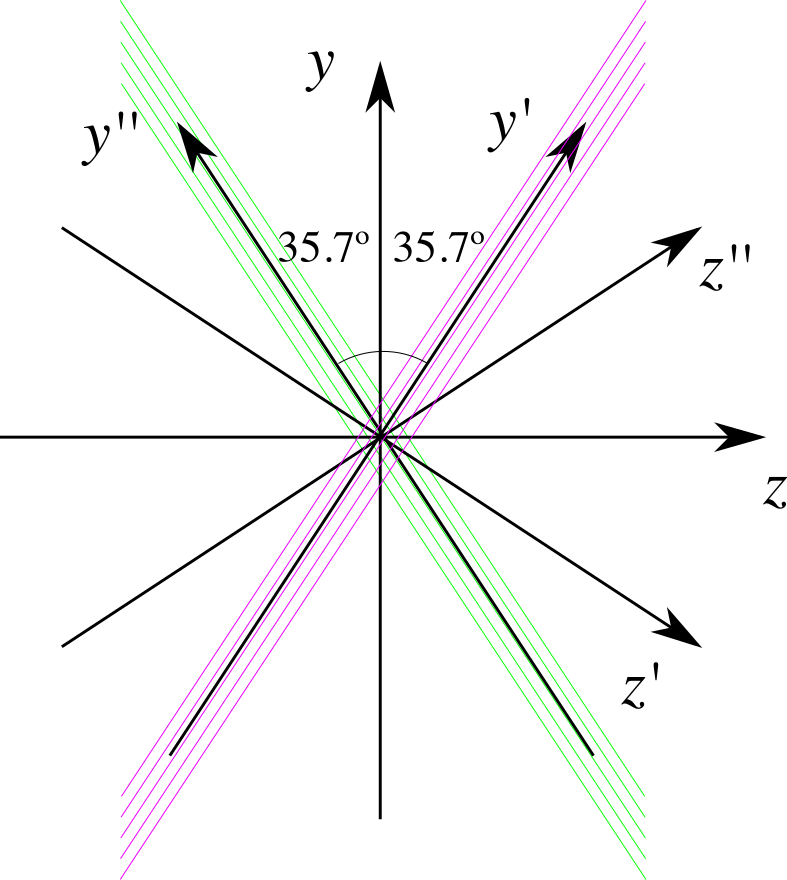
\includegraphics[width=.8\linewidth]{Images/Matched_Filter/sim_rotation}
	\end{subfigure}
	\begin{subfigure}{0.5\textwidth}
		\centering
		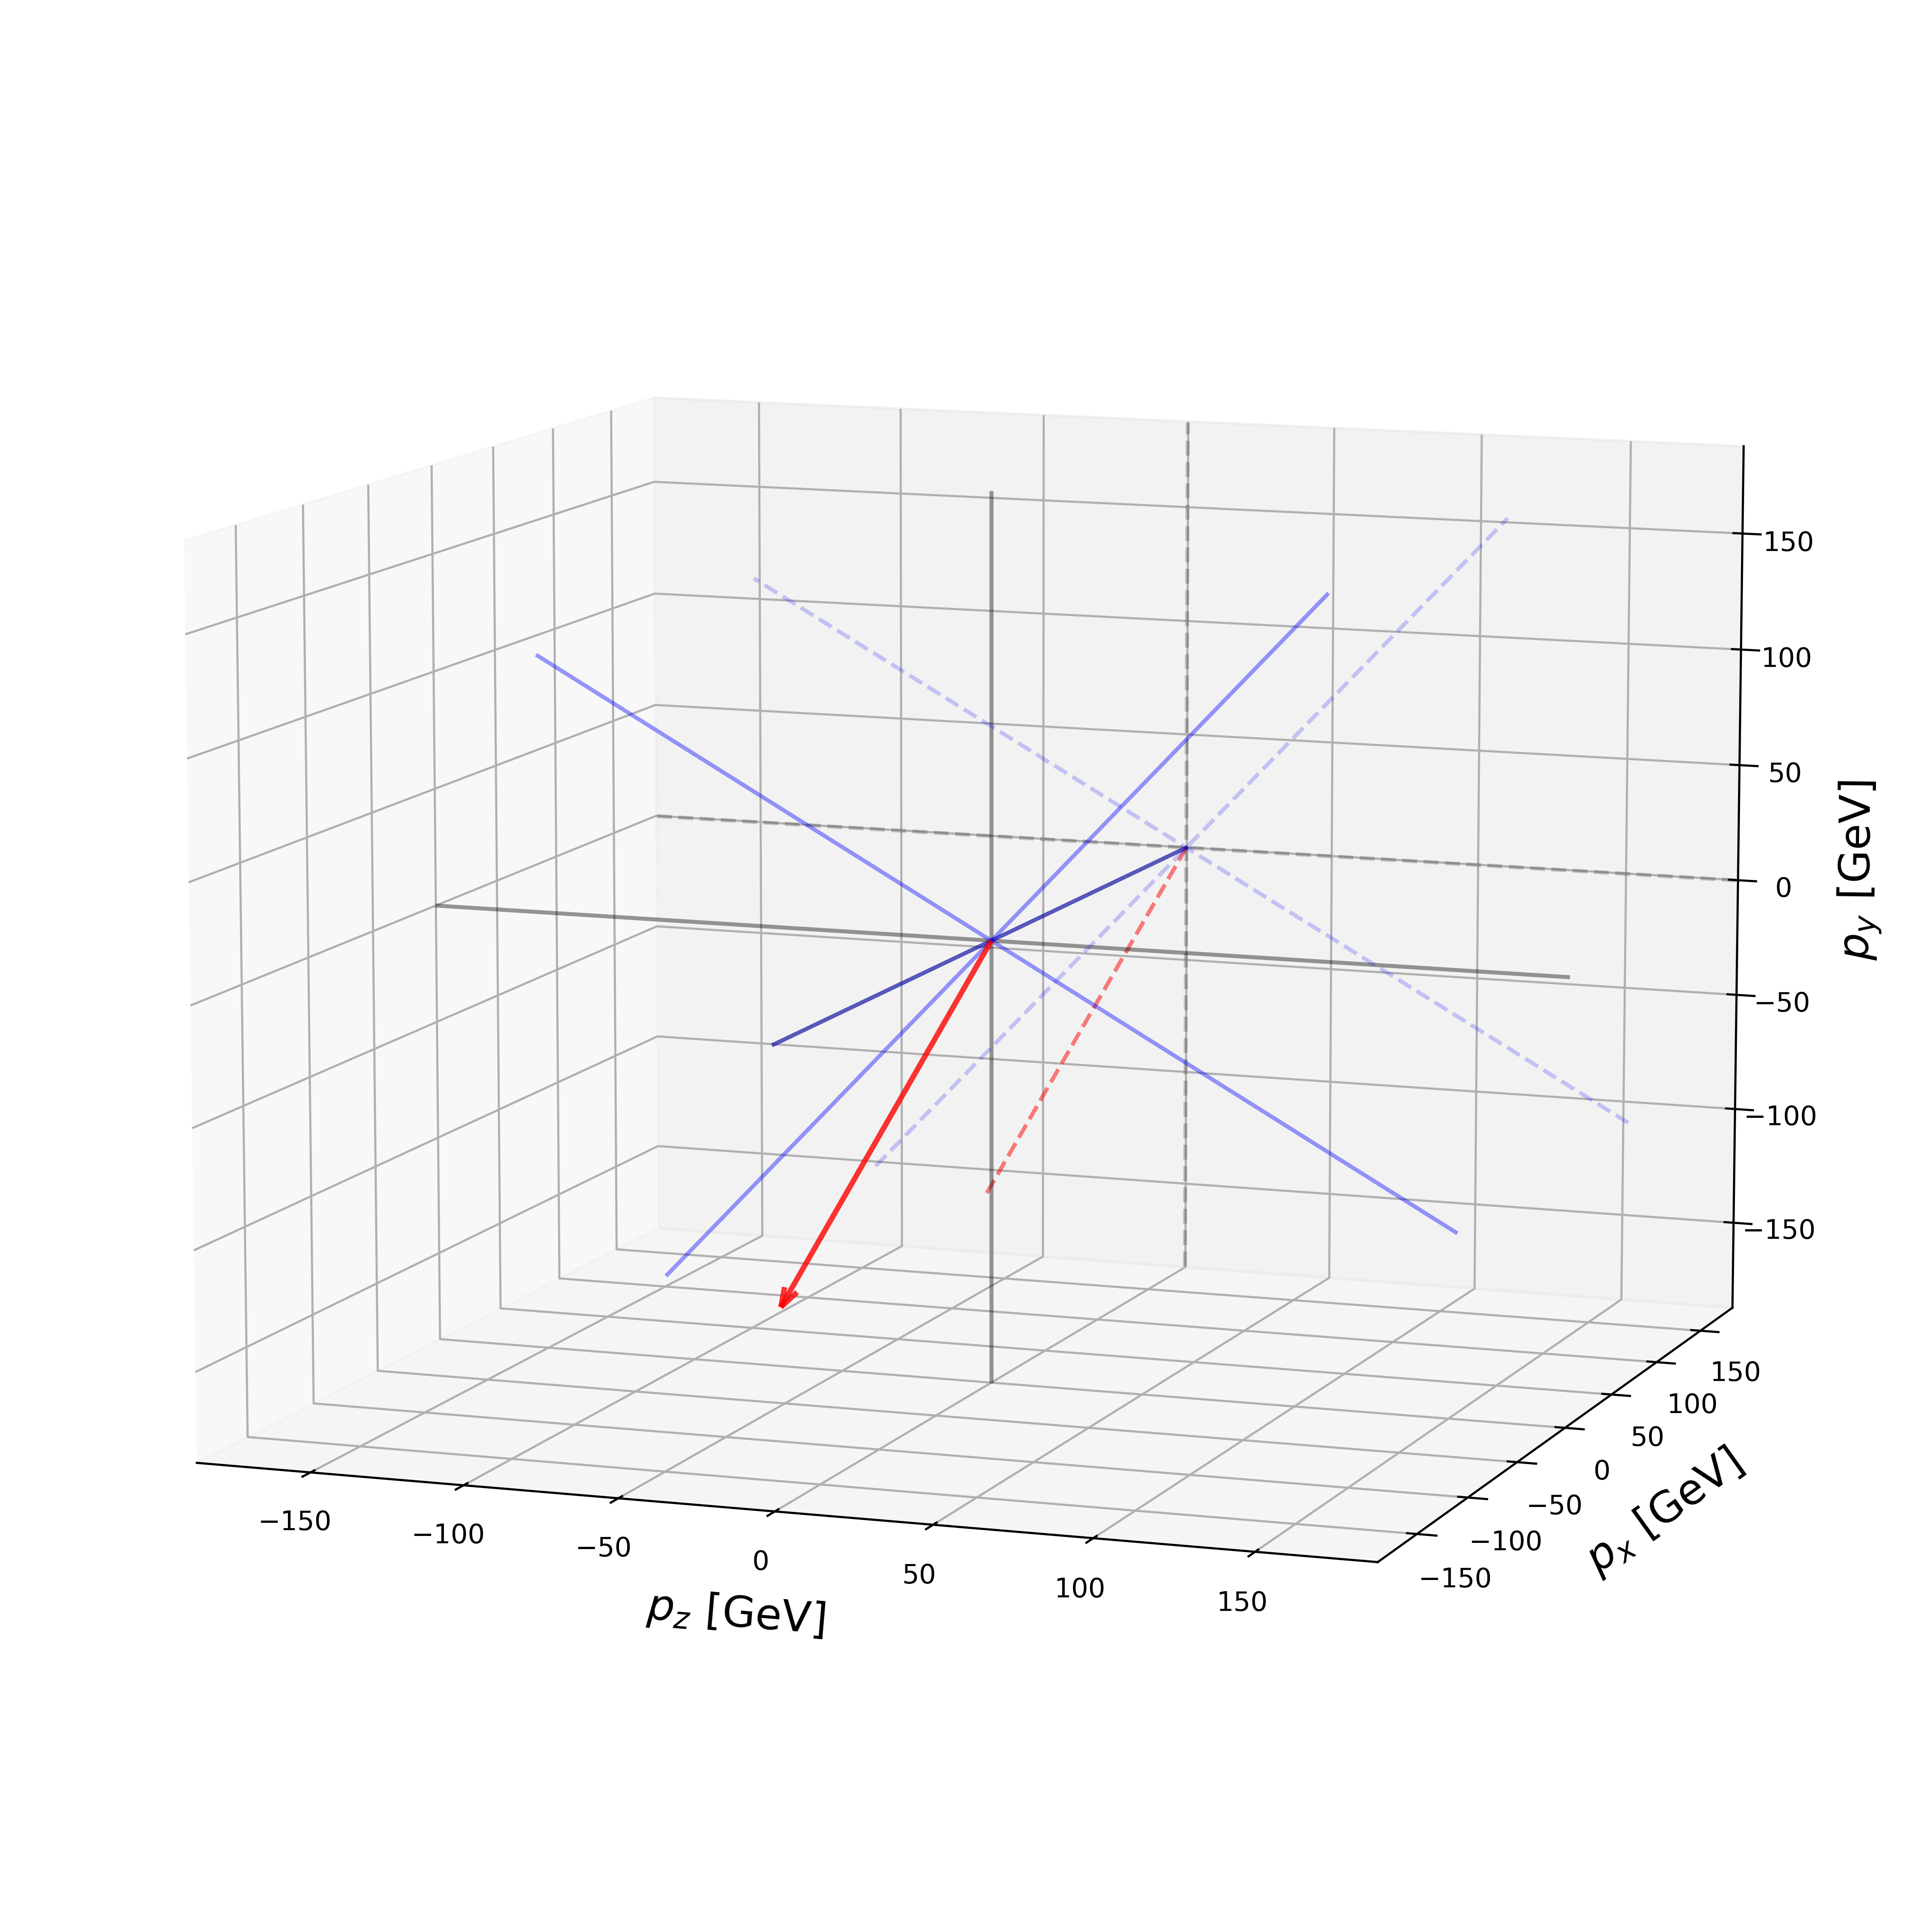
\includegraphics[width=.99\linewidth]{Images/Matched_Filter/3D_rotation}
	\end{subfigure}
	\caption[Schematic representation of the two rotated reference frames used in the analysis of the MC filter performance.]{Left panel: schematic representation of the two new rotated reference frames used in this analysis (denoted as prime and double prime), viewed from the $yz$ plane. The magenta stack of lines represent the wires in the U plane, whereas the green lines correspond to the wires in the V plane. Right panel: 3D representation of the momentum of one of the generated monoenergetic muons (red arrow) in the original reference frame (black lines), along with the new reference frame used for the U plane waveforms (blue lines). In the $yz$ plane I added the projection of these three.}
	\label{fig:reference_frame}
\end{figure}

Additionally, for the analysis of the samples it was necessary to use two different reference frames, to study separately the signals coming from the U and V induction planes. Focussing on a single APA, the U and V channels have a different orientation in the $yz$ plane. In the case of U channels, these are tilted $35.7^{\circ}$ clockwise from the vertical ($y$ direction), whereas the V channels are at the same angle but in the counter-clockwise direction. Because of this, the best option is to deal with two new coordinate systems rotated by $\pm 35.7^{\circ}$ along the $x$ axis, so the new $y'$ and $y''$ directions are aligned with the U and V induction channels, respectively. Figure \ref{fig:reference_frame} (left panel) shows a schematic representation of the original reference frame together with the two rotated ones (denoted by primed and double primed). This way, one can easily understand how parallel was a track to the channels in the two induction planes. Figure \ref{fig:reference_frame} (right panel) shows a 3D representation of the momentum of a track (red arrow) in the original reference frame (black lines), along with the new reference frame for the U plane (blue lines). I added the projections onto the $yz$ plane of these, to show the usefulness of the new reference frame to tell whether a track is parallel or perpendicular to the channels in a induction plane.

\begin{figure}[t]
	\centering
	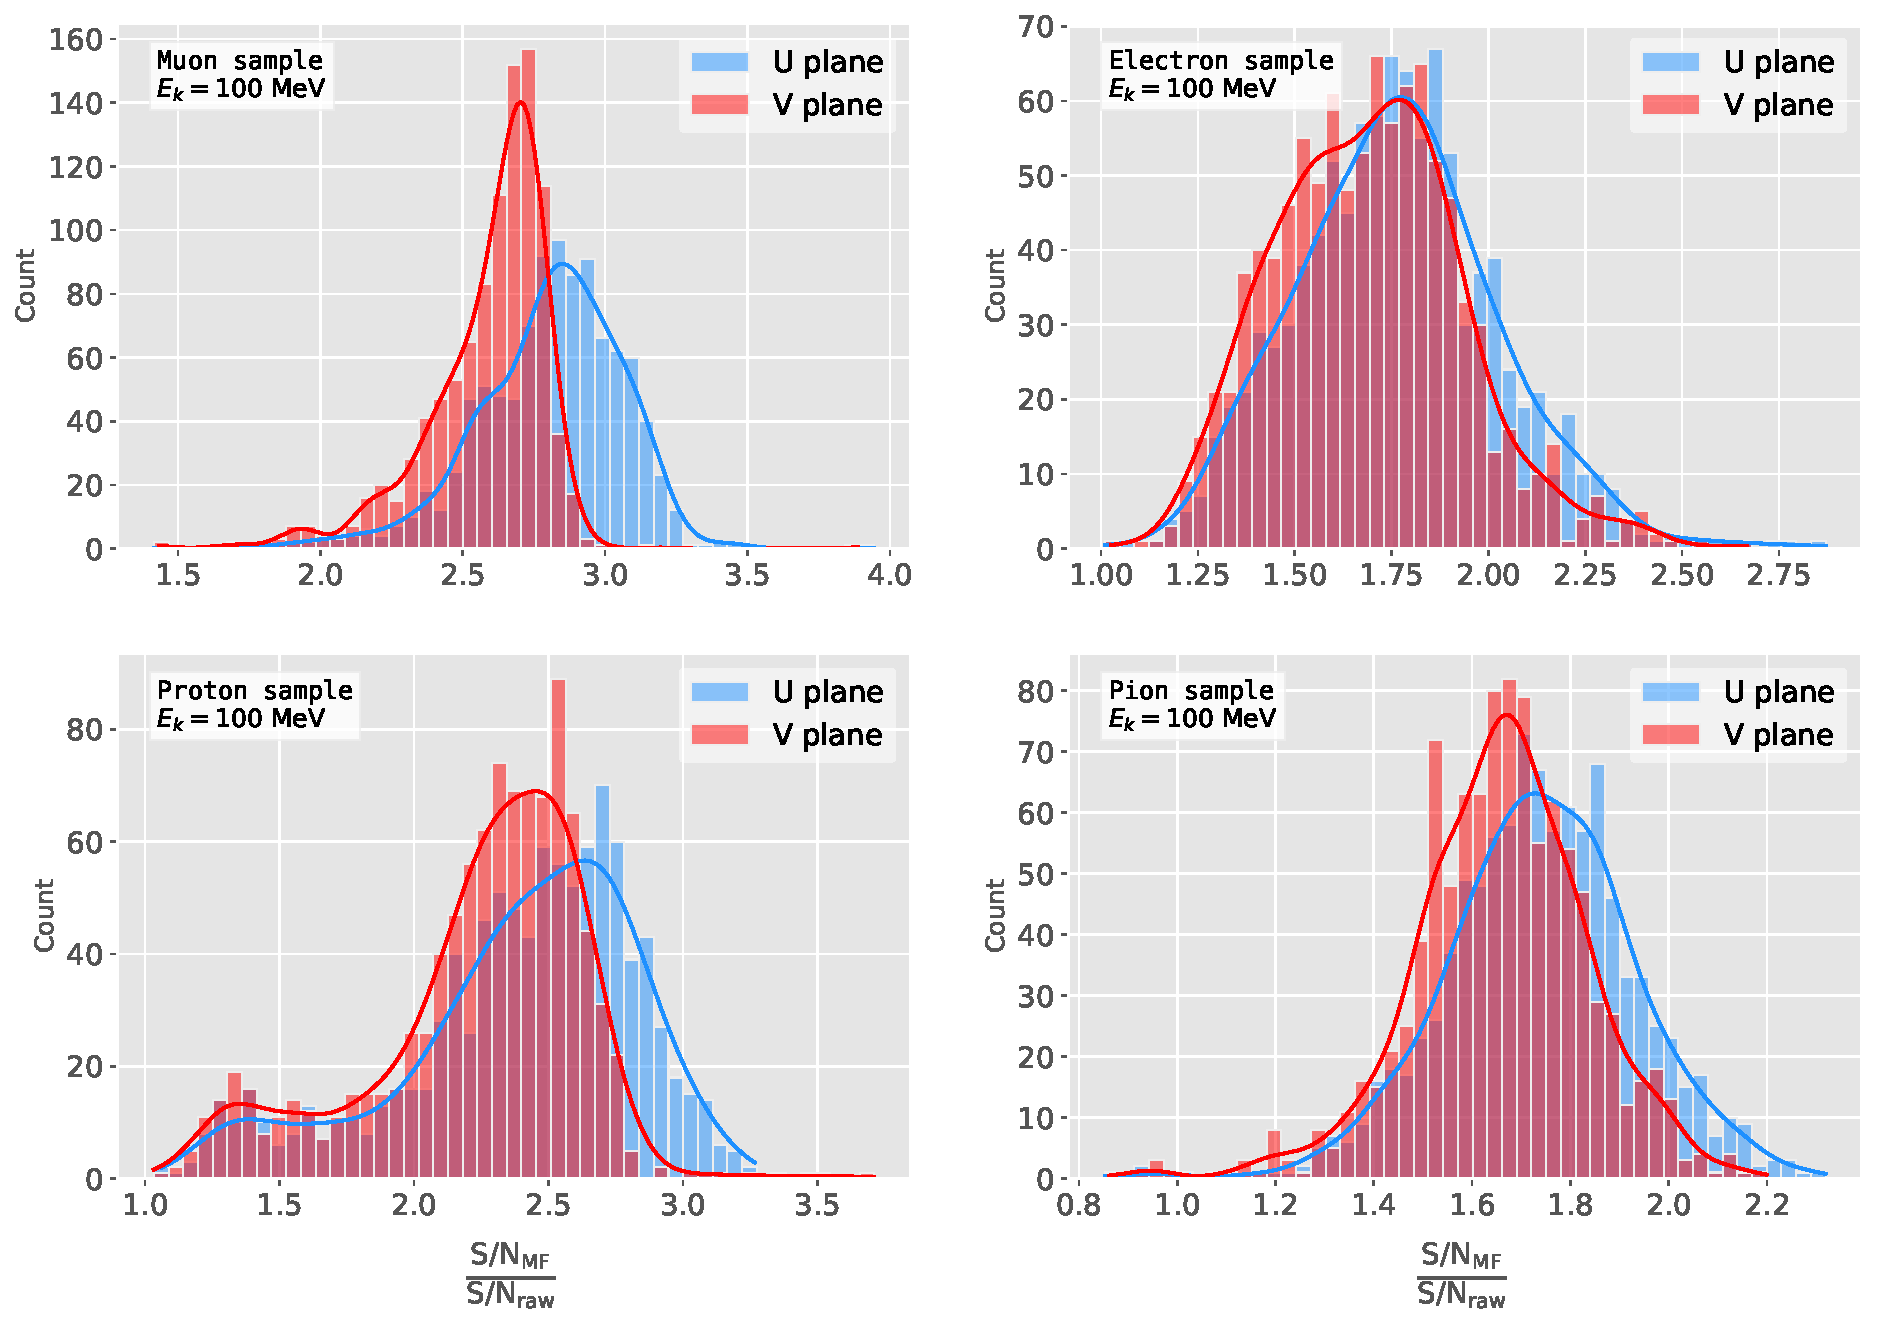
\includegraphics[width=0.9\linewidth]{Images/Matched_Filter/larsoft_sn_hists.pdf}
	\caption[Distributions of the mean S/N change per event for the different MC samples after applying the matched filters.]{Distributions of the mean S/N change per event for the different MC samples after applying the matched filters. Here I separated the change in the U plane (blue) and the V plane (red) channels. From top left to the right: muon, electron, proton and neutral pion. All the events have a fixed kinetic energy of $E_{k} = 100 \ \mathrm{MeV}$.}
	\label{fig:mono_summary_hist}
\end{figure}

Figure \ref{fig:mono_summary_hist} shows the distribution of the average S/N change per event when I apply the optimised matched filters. I produce separate distributions for the channels in the U (red) and V (blue) induction planes. Notice that the S/N distributions for the track-like particles, i.e. muons (top left panel) and protons (bottom left panel), have significantly larger mean values than the distributions of the shower like particles, i.e. electrons (top right panel) and neutral pions (bottom right panel). An important difference between these results and the ones obtained before for the ProtoDUNE-SP data is that the overall improvements that I get with simulated data are more significant. This could be due to an underestimation of the noise levels in the LArSoft simulation. Nonetheless, the concluding message is that the previously optimised matched filters give an overall significant improvement of the S/N for the different samples.

About the convention I follow to present the results results, in the case of the raw and filtered S/N of each event I take the average of these quantities over all the active channels in the event. That is, if a certain event has $N_{chan}$ active channels the two S/N values are computed as:
\begin{equation}
\begin{split}
\left(S/N_{fir}\right)_{event} &= \frac{\sum_{i=0}^{N_{chan}} \left(S/N_{fir}\right)_{i}}{N_{chan}},\\
\left(S/N_{raw}\right)_{event} &= \frac{\sum_{i=0}^{N_{chan}} \left(S/N_{raw}\right)_{i}}{N_{chan}}.
\end{split}
\end{equation}
However, for the ratio of the raw and filtered S/N (what I call the S/N change) per event I do not take the ratio of the previous two quantities but compute the average of the individual ratios per channel in the event:
\begin{equation}
\left(\frac{S/N_{fir}}{S/N_{raw}}\right)_{event} = \frac{\sum_{i=0}^{N_{chan}} \left(\frac{S/N_{fir}}{S/N_{raw}}\right)_{i}}{N_{chan}},
\end{equation}
therefore:
\begin{equation}
\left(\frac{S/N_{fir}}{S/N_{raw}}\right)_{event}  \neq \frac{\left(S/N_{fir}\right)_{event}}{\left(S/N_{raw}\right)_{event}}.
\end{equation}

\subsection{Angular dependence}
\label{subsec:2.5.1}

\begin{figure}[t]
	\centering
	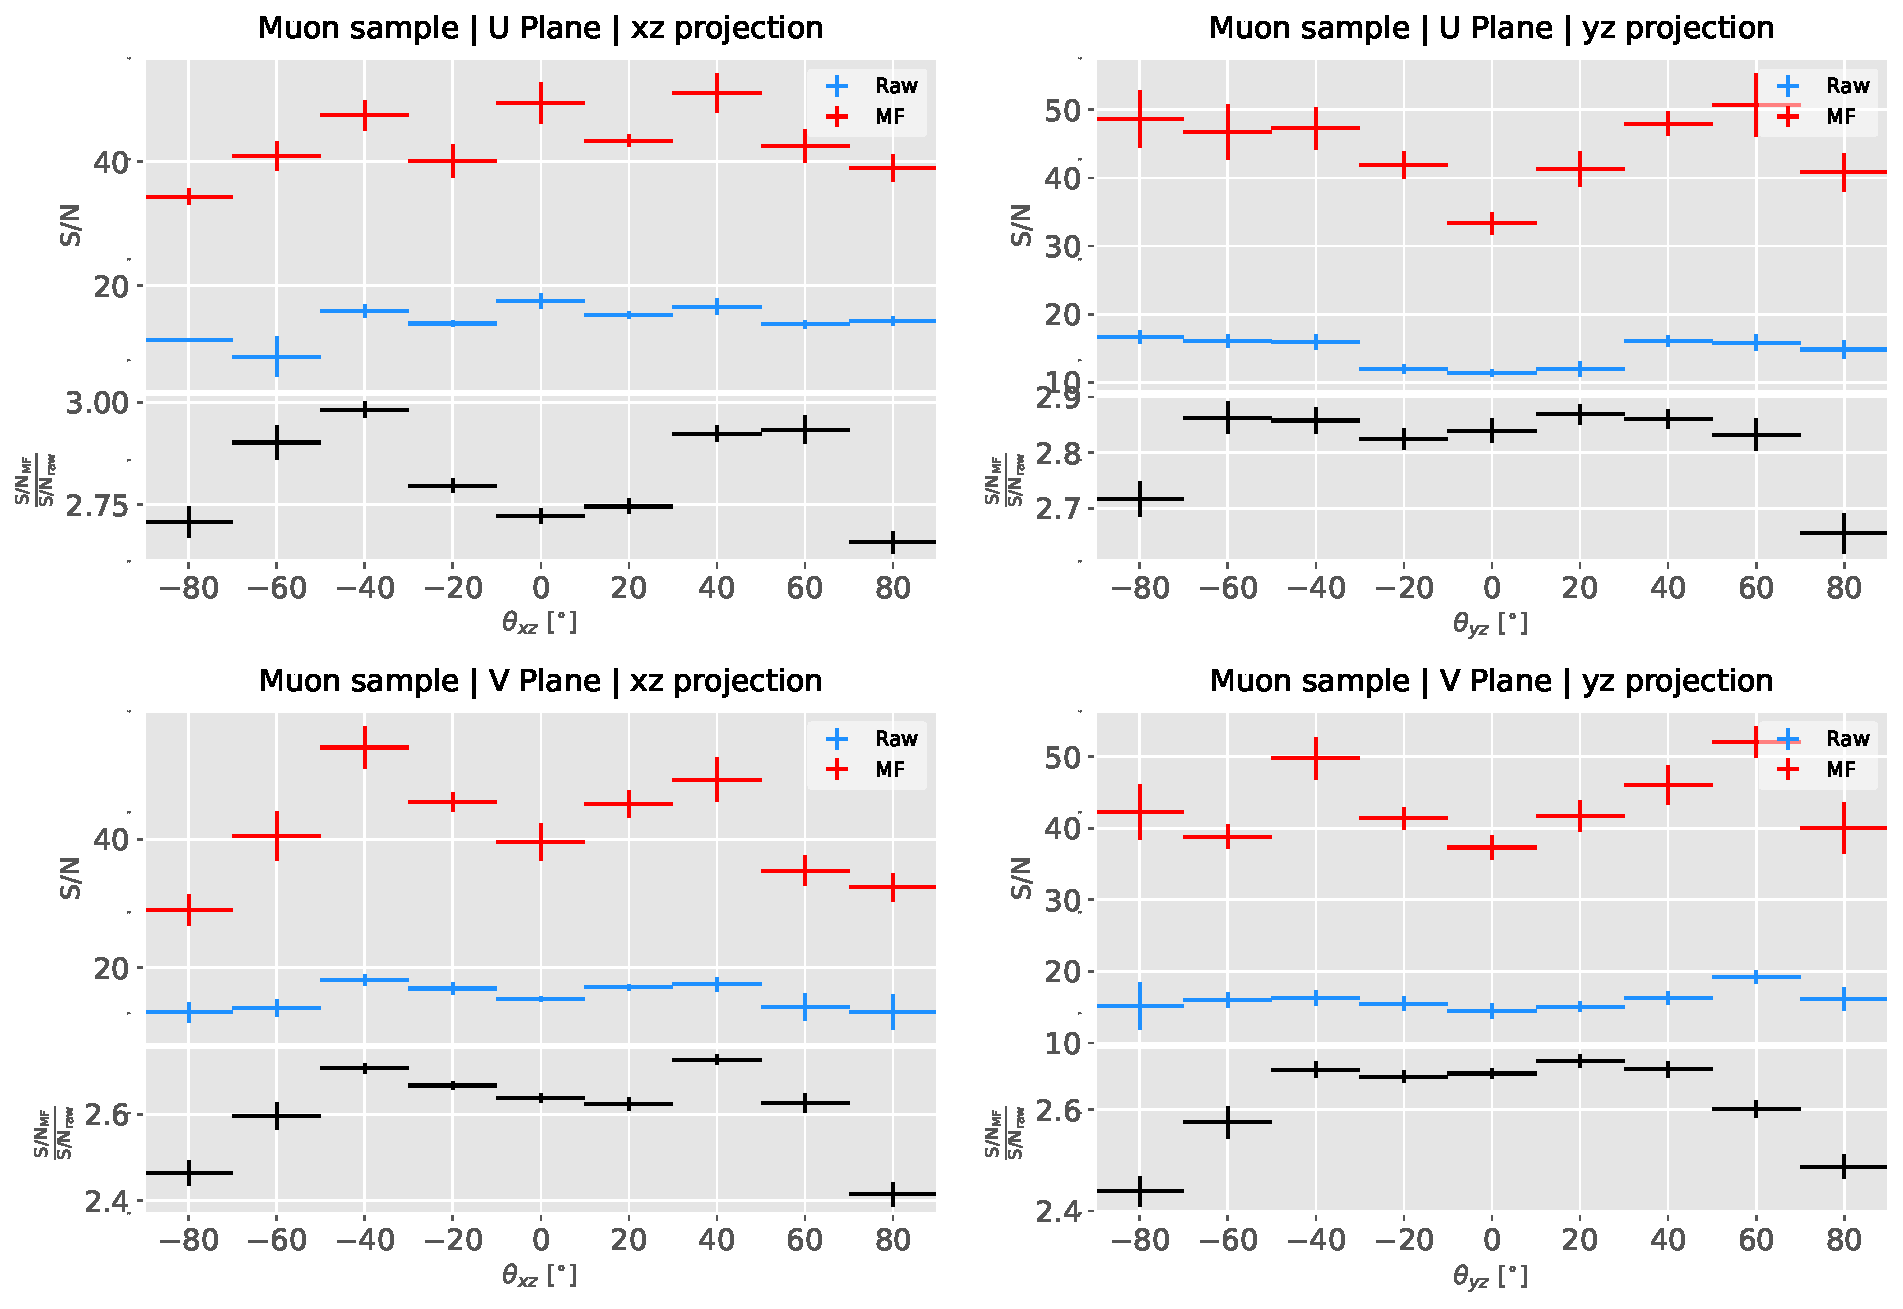
\includegraphics[width=0.9\linewidth]{Images/Matched_Filter/larsoft_muon_angular_alt.pdf}
	\caption[Angular dependence of the mean S/N and the S/N improvement for the monoenergetic muon sample.]{Angular dependence of the mean S/N and the S/N improvement for the monoenergetic muon sample. The top and bottom rows correspond to the U and V planes, respectively. The top subplots show the mean S/N for raw (blue) and filtered (red) waveforms whereas the bottom subplots depict the averaged S/N improvement (black).}
	\label{fig:angular_muon}
\end{figure}

Having these monoenergetic samples, one can study the angular dependence of the matched filter performance. This is an important point, as it is a well established fact that for certain track configurations the S/N is much lower than average as the corresponding waveforms are severely distorted. Therefore, I am interested in seeing how the matched filter behaves in different cases and how the S/N change for those compare to the average.

\begin{figure}[t]
	\centering
	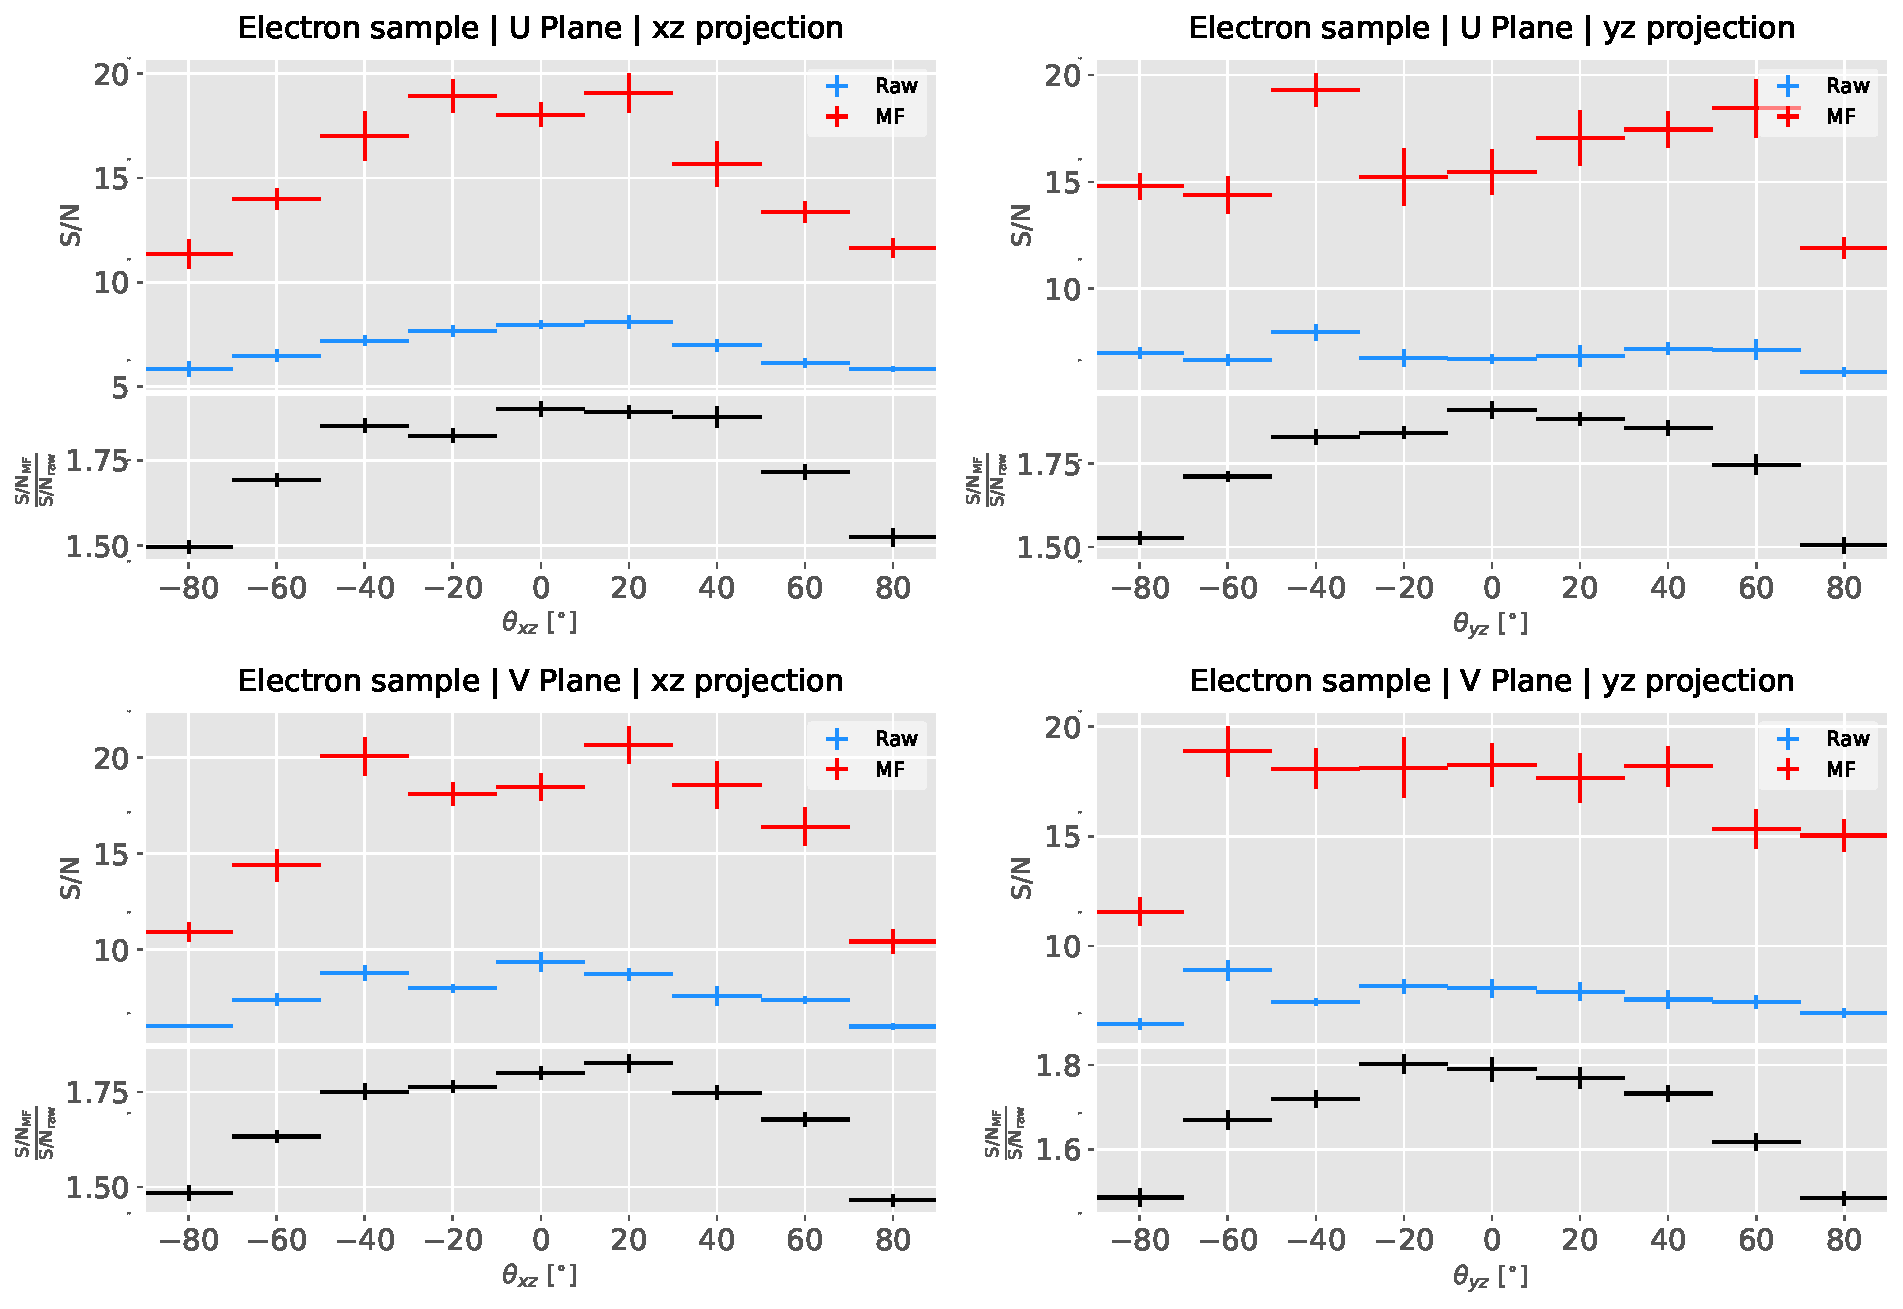
\includegraphics[width=0.9\linewidth]{Images/Matched_Filter/larsoft_electron_angular_alt.pdf}
	\caption[Angular dependence of the mean S/N and the S/N improvement for the monoenergetic electron sample.]{Angular dependence of the mean S/N and the S/N improvement for the monoenergetic electron sample. The top and bottom rows correspond to the U and V planes, respectively. The top subplots show the mean S/N for raw (blue) and filtered (red) waveforms whereas the bottom subplots depict the averaged S/N improvement (black).}
	\label{fig:angular_electron}
\end{figure}

Figure \ref{fig:angular_muon} shows the angular dependence of the S/N for the monoenergetic $E_{k}=100 \ \mathrm{MeV}$ isotropic muons, for the different induction planes and projections. The angles for each event are given by the components of the initial value of the momentum of the particles, taking the angles of the projections on the $xz$ and $yz$ planes with respect to the $z$ axis (more accurately, one needs to compute these angles twice for each event, a pair for the $xy'z'$ coordinate system and the other for the $xy''z''$, as explained previously). The top row shows the dependence on the angles corresponding to the U plane, i.e. $\theta_{xz'}$ and $\theta_{y'z'}$, whereas the bottom row shows the angular dependence viewed from the V plane, $\theta_{xz''}$ and $\theta_{y''z''}$. In each panel, the top subplot represents the mean values of the S/N for the raw (blue) and matched filtered (red) signals, and the bottom subplot the averaged S/N change (black). The horizontal lines show the most probable value for the corresponding angular bin, obtained from a fit to a Landau distribution. The vertical lines represent the error in the parameter estimation.

Both for the raw and matched filtered samples, the S/N is lower for tracks that are normal to the APA ($\theta_{xz} \sim \pm 90^{\circ}$). Similarly, tracks parallel to the wires ($\theta_{yz} \sim \pm 90^{\circ}$) tend to have higher S/N than those perpendicular to these ($\theta_{yz} \sim 0$). The S/N improvement seems to follow similar trends for both projections in the two planes. In the $xz$ plane there is a slight preference for tracks with $\theta_{xz} \sim \pm 45^{\circ}$ (particularly in the U plane), whereas in $yz$ the S/N change plateaus around the central region.

Figure \ref{fig:angular_electron} shows the corresponding angular dependence results for the $E_{k}=100 \ \mathrm{MeV}$ electrons sample. Although the S/N behaviour in this case is similar to what I observed for the muons, some differences are evident. A possible explanation can be that, because a significant fraction of the hits in these events are produced by the secondary particles generated in the EM shower, some of the S/N ratios do not correspond to the directional information of the primary electron. Even so, the S/N change distribution exhibits a consistent pattern and it is clear that the matched filter enhances the signal regardless of the electron direction.

\begin{comment}
\begin{figure}[t]
	\begin{subfigure}{0.5\textwidth}
		\centering
		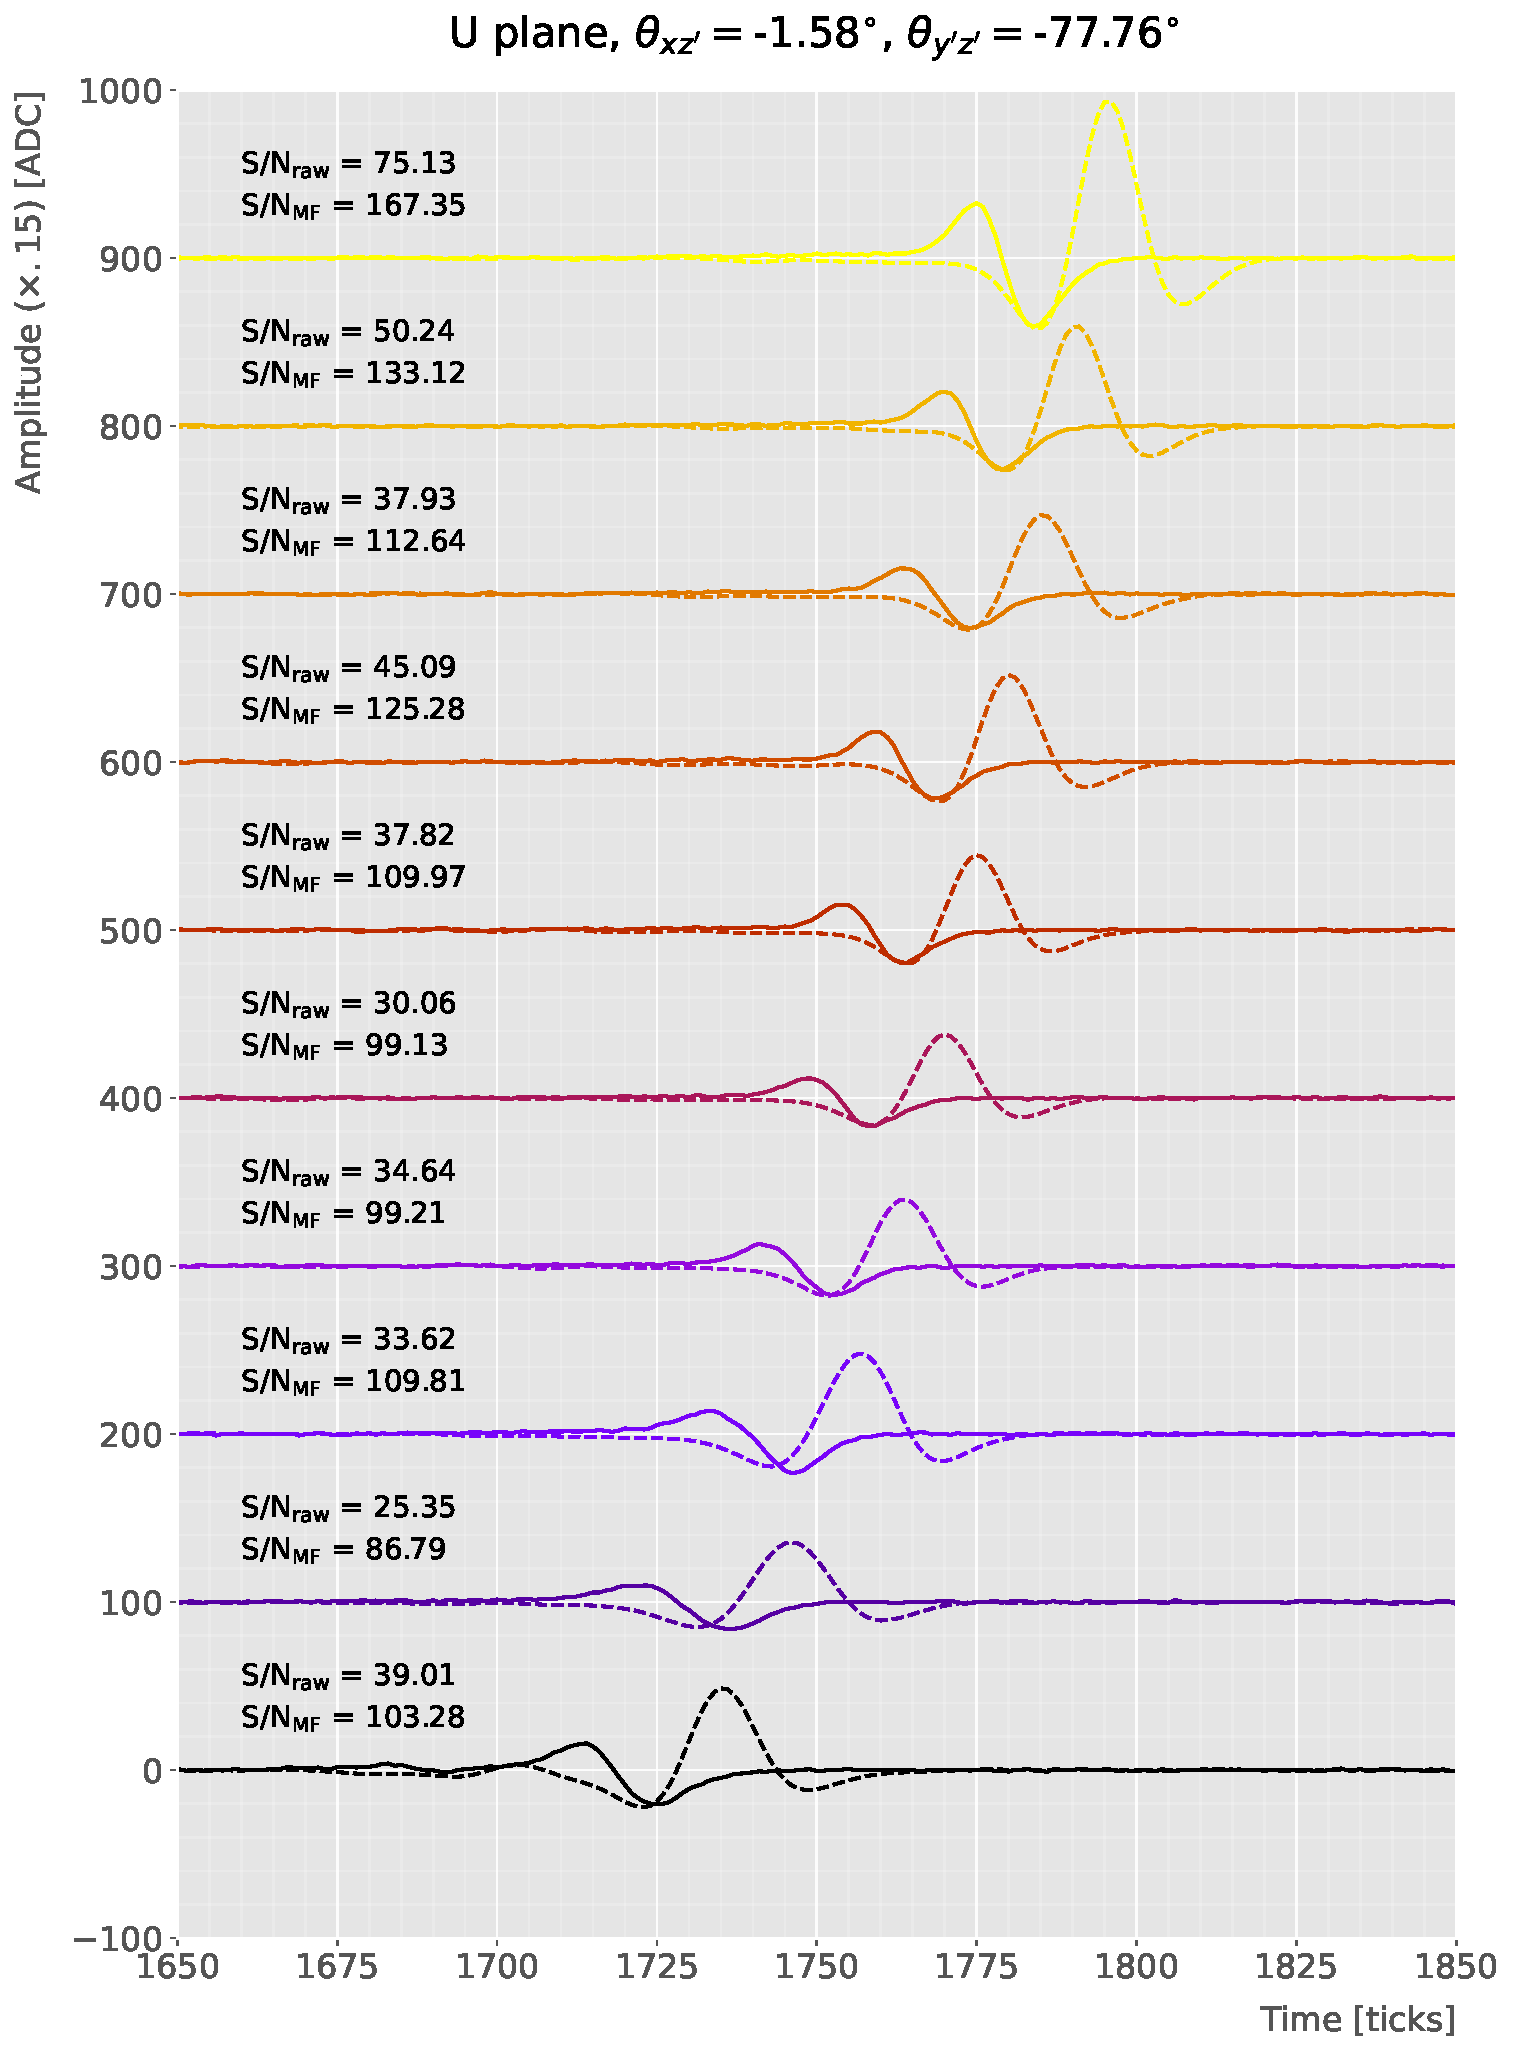
\includegraphics[width=.99\linewidth]{Images/Matched_Filter/evt_xz_0_yz_90_U}
	\end{subfigure}
	\begin{subfigure}{0.5\textwidth}
		\centering
		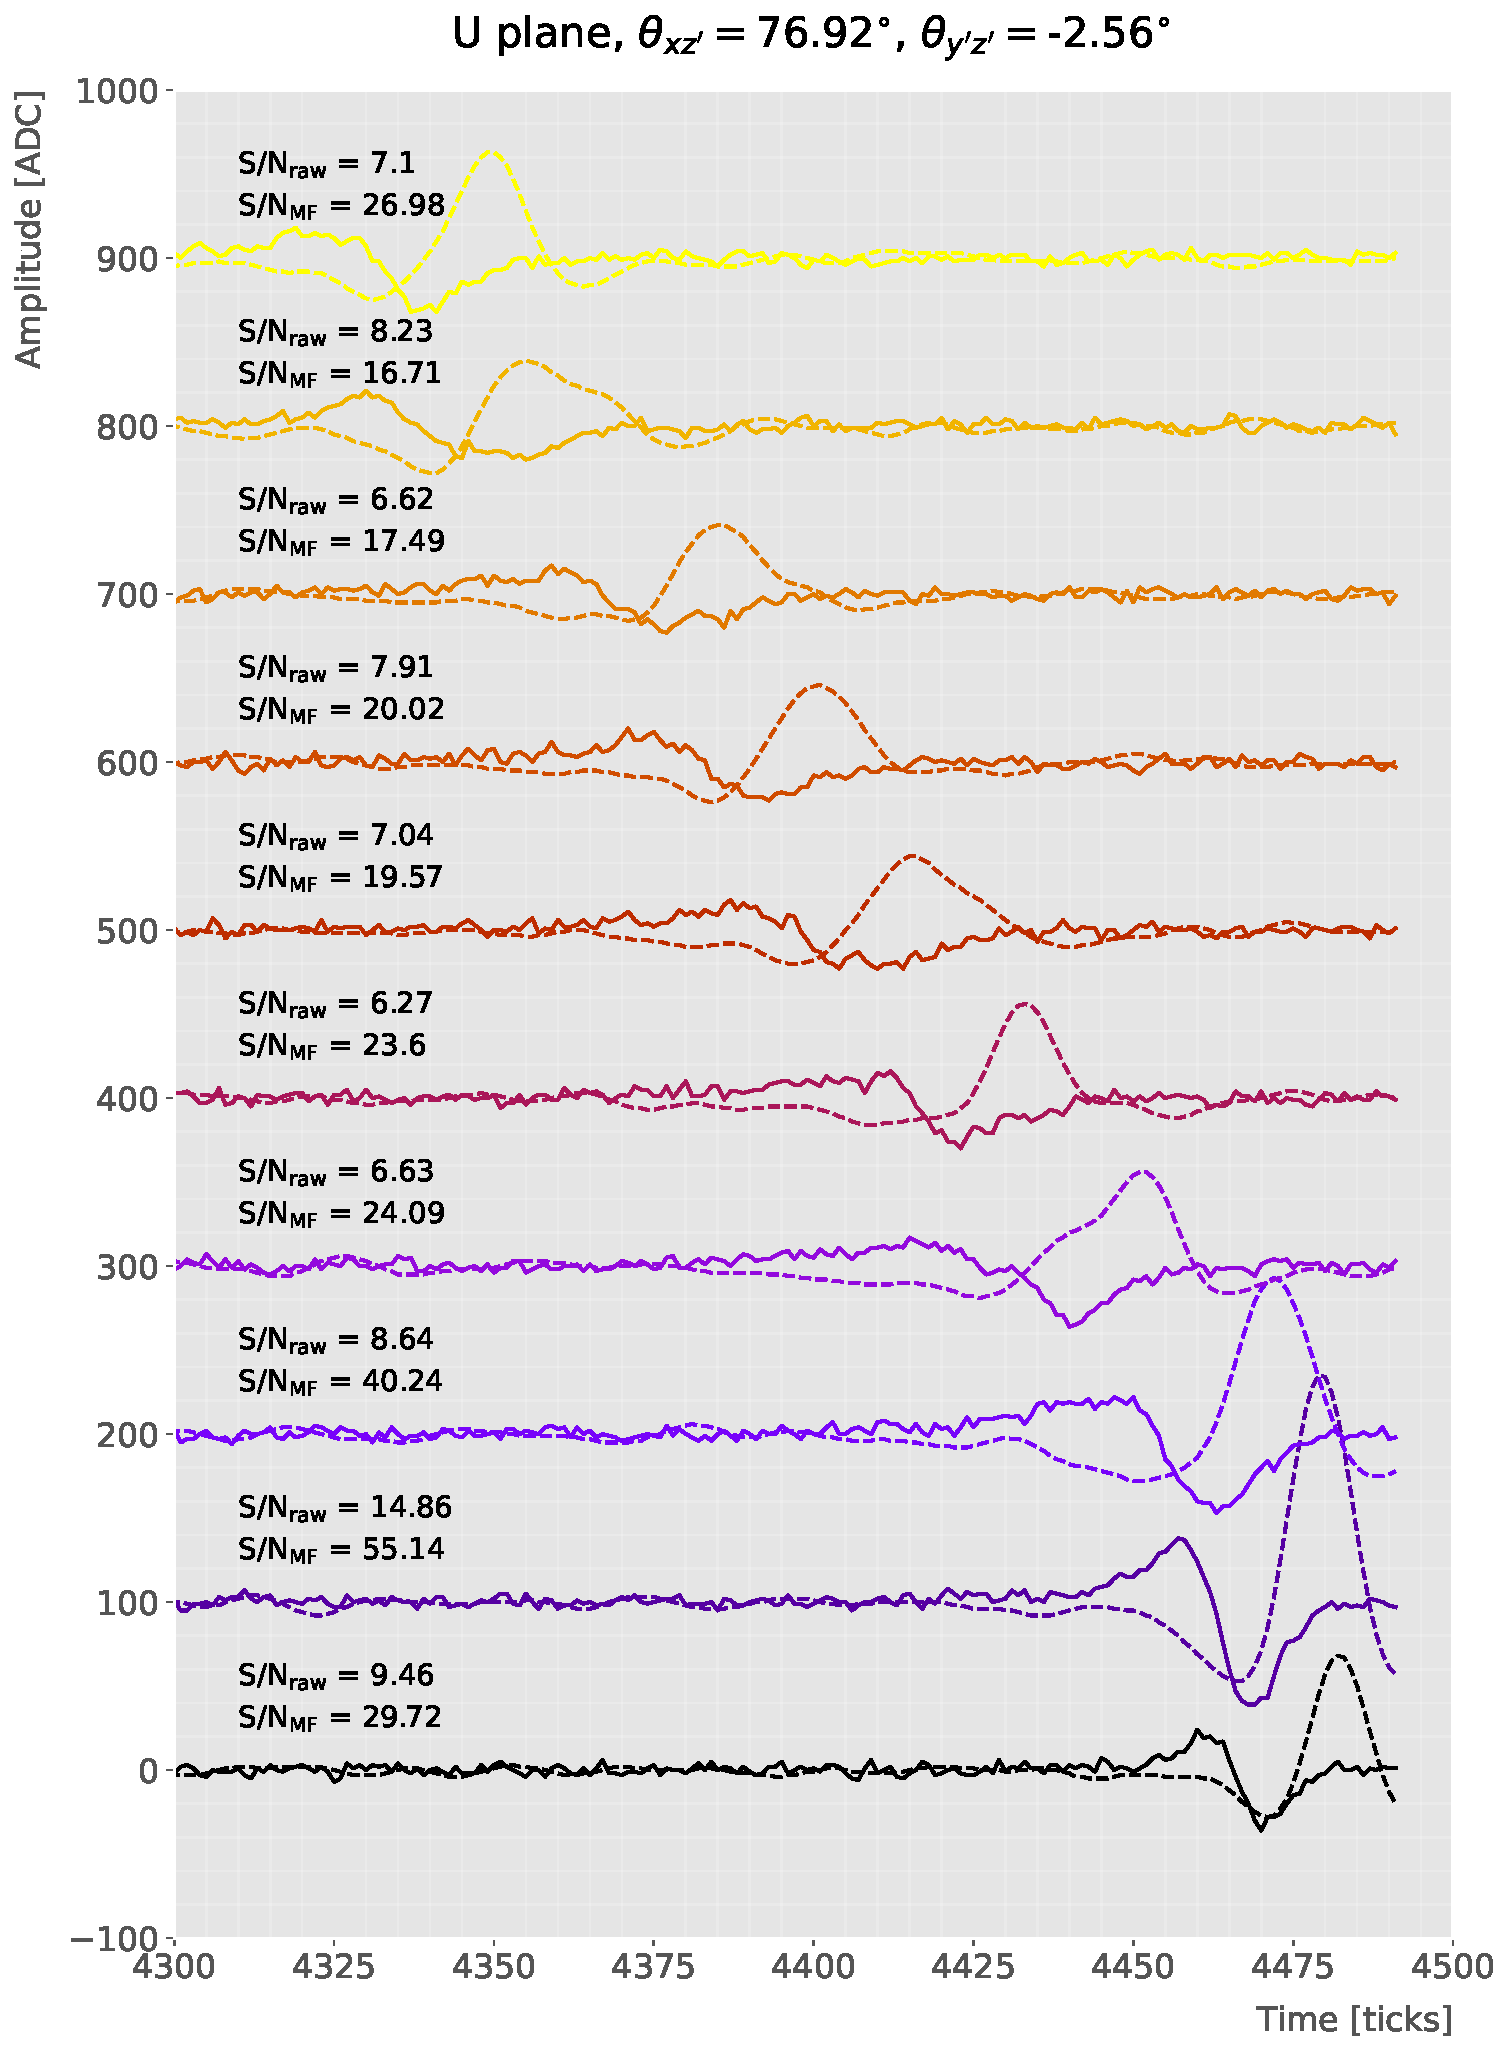
\includegraphics[width=.99\linewidth]{Images/Matched_Filter/evt_xz_90_yz_0_U}
	\end{subfigure}
	\caption[Waveforms for two muon events, one parallel to the APA and to the wires in the U plane and other normal to the APA plane and perpendicular to the U plane wires.]{Selected consecutive waveforms corresponding to two monoenergetic $E_{k} = 100 \ \mathrm{MeV}$ muon events, one is parallel to the APA and to the wires in the U plane (left panel) and the other is normal to the APA plane and perpendicular to the U plane wires (right panel). The solid lines represent the raw waveforms whereas the dashed lines correspond to the waveforms after the matched filter was applied. The waveforms on the left panel have been scaled by a factor of $0.15$ to have similar amplitudes to the ones on the right panel.}
	\label{fig:example_orientation}
\end{figure}

\subsection{Distortion and peak asymmetry}
\label{sec:A.5}

As a case study, I select two of the simulated $E_{k} = 100 \ \mathrm{MeV}$ monoenergetic muon events. With respect to the U induction plane, one is parallel to the APA (low $\theta_{xz'}$) and to the wires (high $\theta_{y'z'}$) and the other is normal to the APA plane (high $\theta_{xz'}$) and perpendicular to the wires (low $\theta_{y'z'}$). As expected from the results on the angular dependence discussed above, the former has a higher S/N (both before and after the filtering) when compared to the latter. An interesting thing to notice about these two samples is that, even though one has a much larger S/N than the other, it is the one with the smallest S/N the one that gets a more significant averaged S/N improvement. In Tab. \ref{tab:case} I include all the relevant parameters of these two $E_{k} = 100 \ \mathrm{MeV}$ muon events, namely the angles with respect to the $xy'z'$ reference frame, the values of the S/N, the S/N change and also the so-called peak asymmetry $\Delta_{peak}$, that I will define next.

\begin{figure}[t]
	\begin{subfigure}{0.5\textwidth}
		\centering
		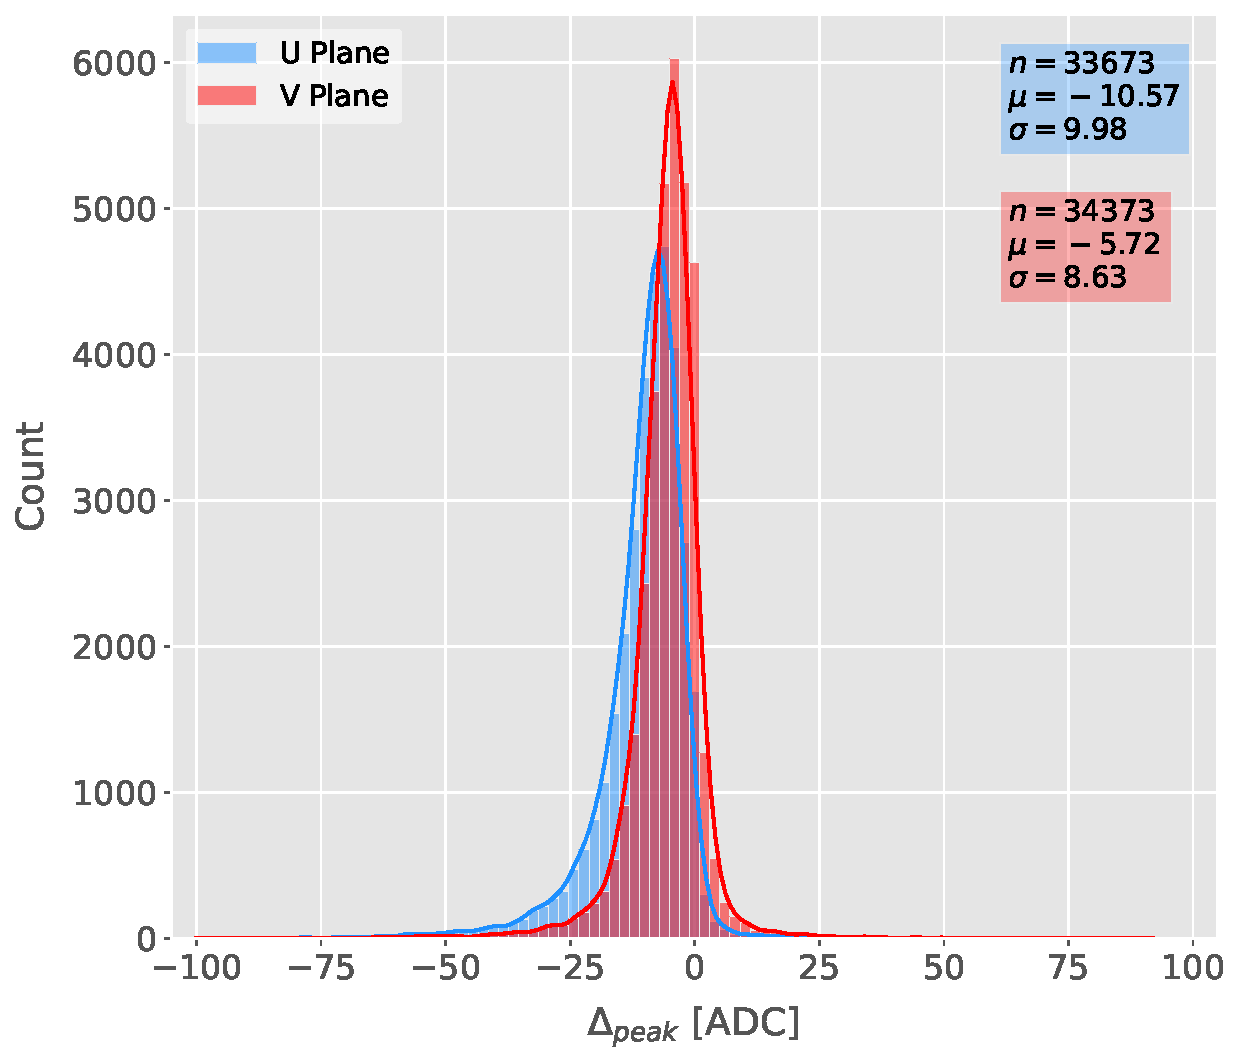
\includegraphics[width=.99\linewidth]{Images/Matched_Filter/deltaPeak_dist}
	\end{subfigure}
	\begin{subfigure}{0.5\textwidth}
		\centering
		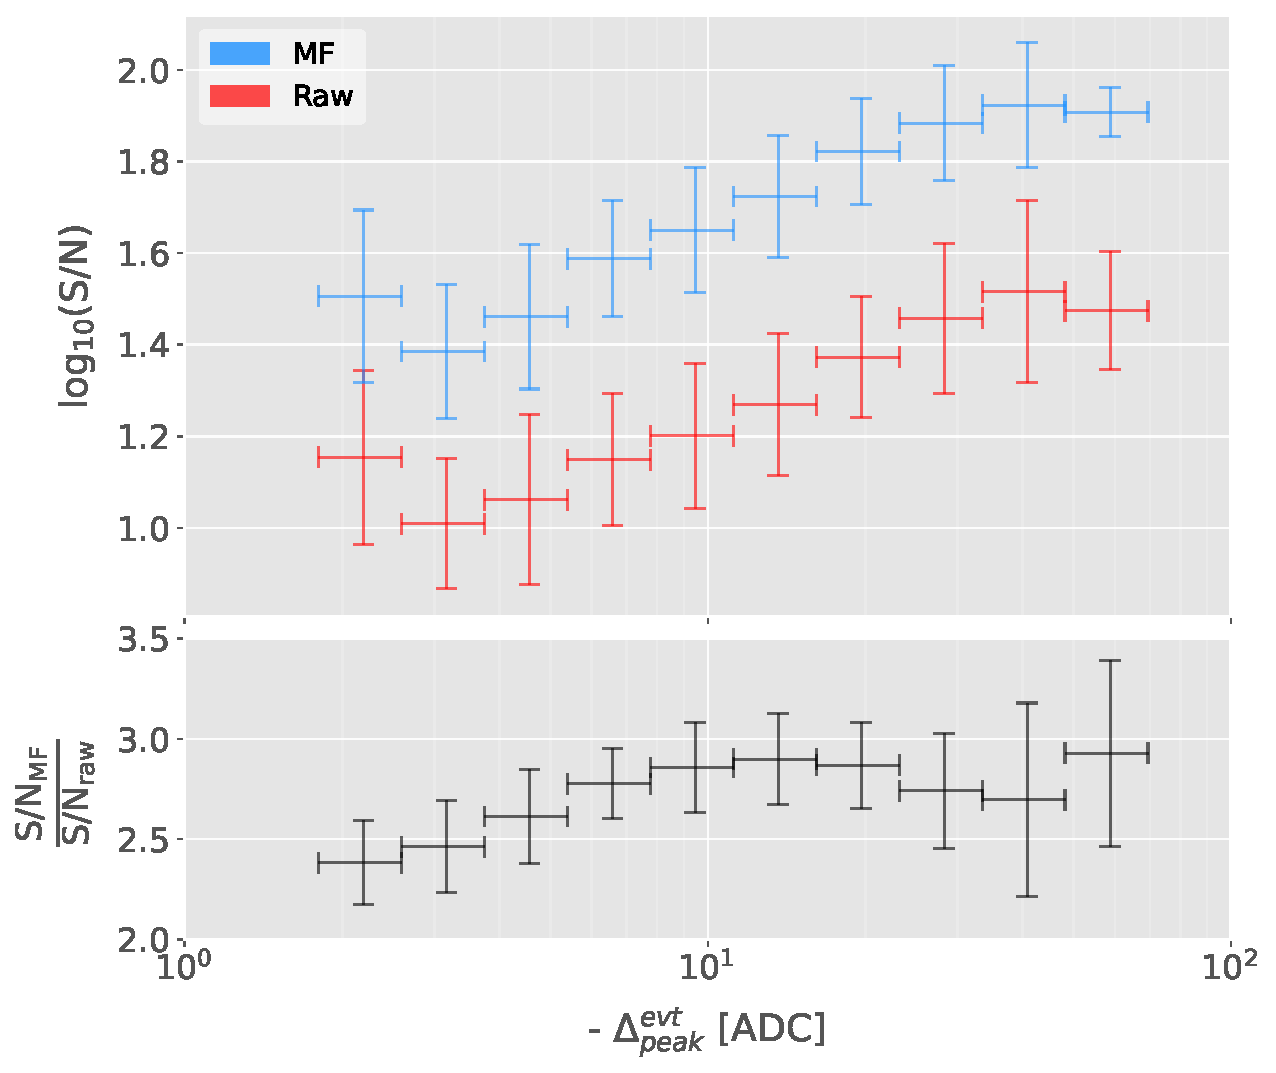
\includegraphics[width=.99\linewidth]{Images/Matched_Filter/deltaPeak_SN_ratio}
	\end{subfigure}
	\caption[Distribution of the peak asymmetry for the monoenergetic muon sample and dependence of the S/N change on the mean peak asymmetry of the event.]{Left panel: peak asymmetry distribution for the case of the monoenergetic $E_{k} = 100 \ \mathrm{MeV}$ muon sample. Each value corresponds to a single bipolar signal peak from a channel in any event. The blue distribution represents the peaks on U plane channels, whereas the red corresponds to signal peaks in V wires. Right panel: relation between the mean peak asymmetry per event with the S/N for U channel waveforms from the $E_{k} = 100 \ \mathrm{MeV}$ muon sample. The top subplot shows the decimal logarithm of the mean S/N for the raw (red) and the matched filtered (blue) waveforms. The bottom subplot contains the mean S/N improvement ratio after the matched filter was applied.}
	\label{fig:asymmetry}
\end{figure}

\begin{table}[h!]
	\centering
	\caption[Characteristic parameters of the two monoenergetic muon events selected for the peak asymmetry study.]{Characteristic parameters of the two monoenergetic muon events selected, relative to the U plane: projected angles in the $xz'$ and $y'z'$ planes, S/N values for the raw and filtered waveforms, mean improvement of the S/N and peak asymmetry.}
	\begin{tabular}{l|llllll}
		& $\theta_{xz'} \ (^{\circ})$ & $\theta_{y'z'} \ (^{\circ})$ & $\mathrm{S/N}_{\mathrm{raw}}$ & $\mathrm{S/N}_{\mathrm{MF}}$ & $\frac{\mathrm{S/N}_{\mathrm{MF}}}{\mathrm{S/N}_{\mathrm{raw}}}$ & $\Delta_{peak} \ (\mathrm{ADC})$ \\[2mm] \hline
		\rule{0pt}{1.1\normalbaselineskip}High (``parallel'') & -1.58                     & -77.76                     & 41.65       & 112.44      & 2.83                          & -35.73                                                          \\[2mm]
		Low (``normal'')  & 76.92                     & -2.56                      & 8.07        & 25.46       & 3.12                          & -10.38                                                         
	\end{tabular}
	\label{tab:case}
\end{table}

One can try to understand better the nature of these two events by looking at the raw and filtered data from some of their active channels. Figure \ref{fig:example_orientation} shows a selection of consecutive raw and filtered U plane waveforms from the event with high S/N (left panel) and the one with low S/N (right panel). To show both collections of waveforms at a similar scale I had to apply a factor of $0.15$ to the waveforms with high S/N. Additionally, next to each waveform I include the values of the raw and matched filtered S/N for the corresponding channel. The first thing to notice is that the amplitude of the signal peaks from the normal track have a much smaller amplitude, and also appear quite distorted when compared to the others. On the other hand, although the matched filtered S/N for each channel are still smaller, the relative improvements are larger than in the parallel case.

A way to quantify the difference between the shape of the waveforms of these two events is using their peak asymmetry. I define the peak asymmetry as the (signed) difference between the positive and the negative peaks of the bipolar shape, i.e.:
\begin{equation}
\Delta_{peak} \equiv h_{+} - h_{-},
\end{equation}
where both heights $h_{+}$ and $h_{-}$ are positive. Figure \ref{fig:asymmetry} (left panel) shows the distribution of this peak asymmetry for all the waveforms corresponding to channels in the U (blue) and V (red) planes for the monoenergetic muon sample. One can see that these distributions are clearly shifted to negative values, with means $\mu_{\Delta}^{\mathrm{U}} = -10.57 \ \mathrm{ADC}$ and $\mu_{\Delta}^{\mathrm{V}} = -5.72 \ \mathrm{ADC}$, respectively. Notice how the peak asymmetry value of the selected event with the high S/N sits at the left tail of the distribution, whereas the corresponding value of the sample with the low S/N lies around the mean.

It is possible to correlate the peak asymmetry with the S/N and the S/N change per event. Figure \ref{fig:asymmetry} (right panel) shows the result of comparing the mean peak asymmetry per event to the averaged raw (red) and matched filtered (blue) S/N per event (top subplot). The horizontal lines sit at the mean value obtained in the fit and represent the width of the $-\Delta_{peak}$ bins used, while the vertical lines indicate one standard deviation around that mean value. Notice how there is an approximate linear relation between the peak asymmetry and the S/N, except for peak asymmetry values bigger than $- 5 \ \mathrm{ADC}$ where the S/N remains constant.

Also, in the bottom subplot of Fig. \ref{fig:asymmetry} (right panel) I show the relation between the peak asymmetry and the mean S/N change. In this case, one can see that there is a clear maximum at $\Delta_{peak} \sim -10 \ \mathrm{ADC}$. As mentioned previously, this is also the value of the mean of the peak asymmetry distribution. In fact, it is expected that our filter favours the signal peaks with the most common values of the peak asymmetry, as this was one of the features I target in our filter coefficient optimisation through the parameter $\delta$.

These results suggest that events with poorer values of the mean S/N, usually associated to non-favourable track orientations, tend to have smaller values of the mean peak asymmetry (in absolute value). Nonetheless, because our matched filters have been optimised to account for these asymmetries, the improvement on the S/N for these events is sizeable if not better than the one for events which already had a high S/N.
\end{comment}

\subsection{Hit sensitivity}
\label{subsec:2.5.3}

\begin{figure}
	\centering
	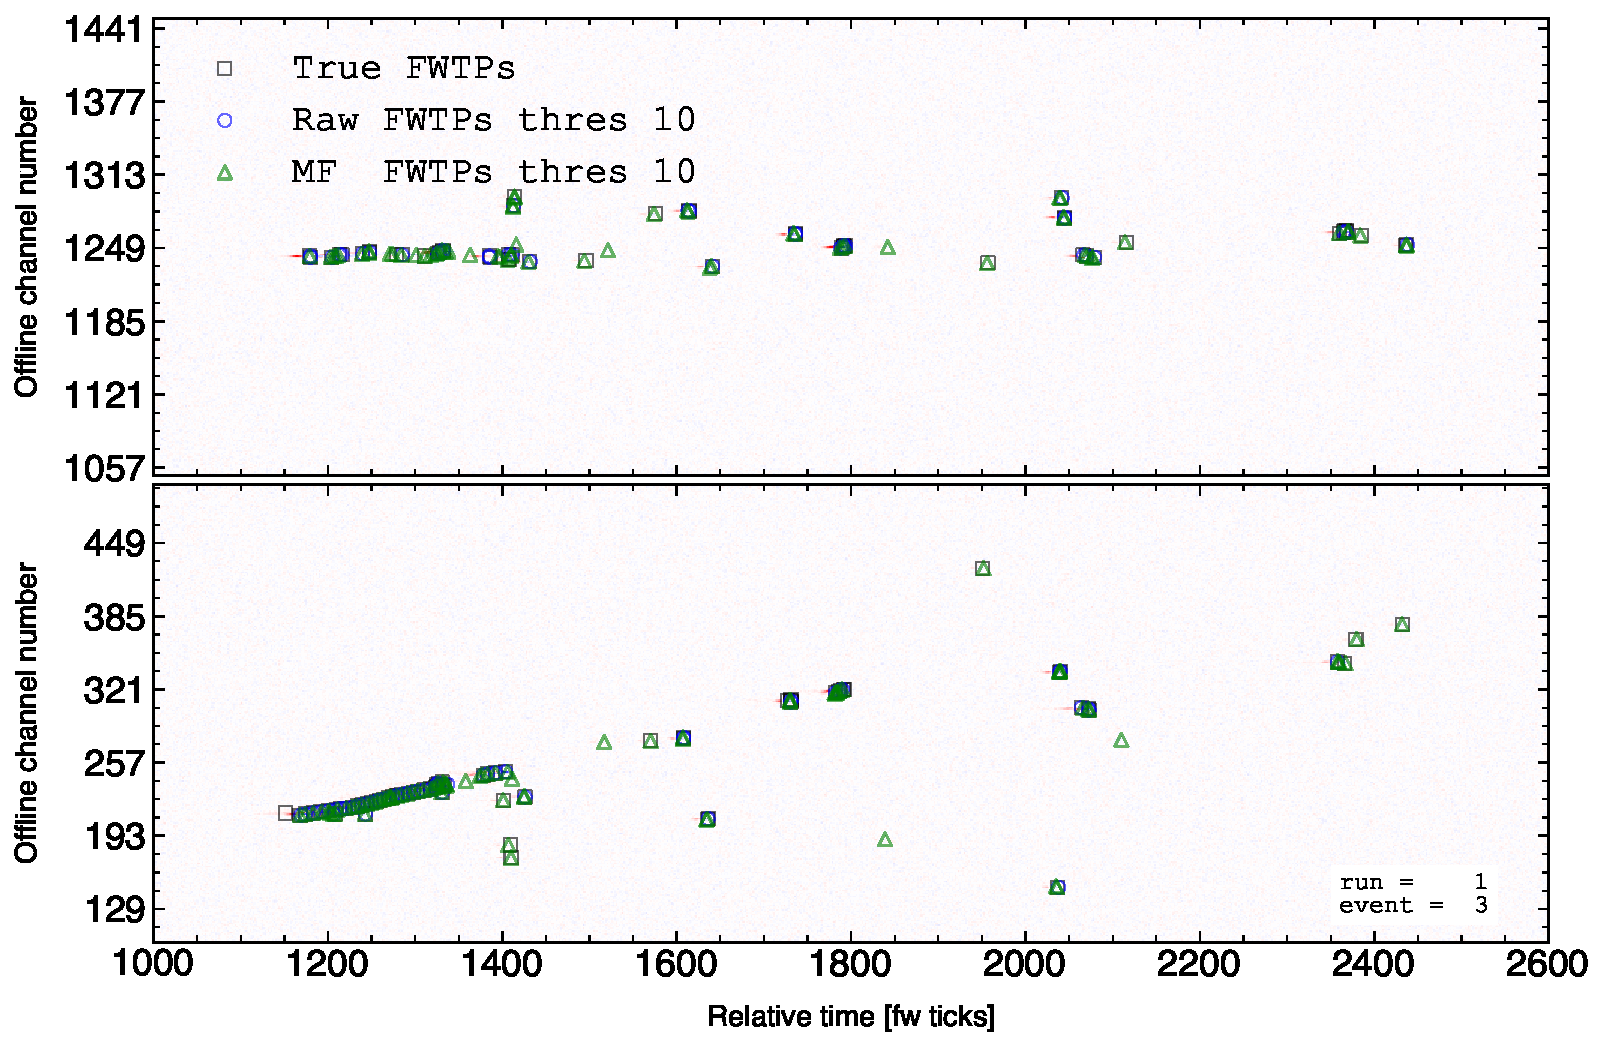
\includegraphics[width=0.9\linewidth]{Images/Matched_Filter/electron_k100_full_run_1_evt_3}
	\caption[Raw event display for an electron event showing the true, standard, and matched filter hits produced.]{Raw event display showing the time (in firmware ticks) versus offline channel number for a $E_{k} = 100 \ \mathrm{MeV}$ electron event. The produced true hits are superimposed (black boxes) as well as the hits coming from the standard hit finder chain (blue circles) and the hit finder using the matched filter (green triangles).}
	\label{fig:evthitcomp}
\end{figure}

One of the advantages of the matched filter, directly related to increasing the S/N, is the capability of forming TPs that before fell below the threshold. For instance, Fig. \ref{fig:evthitcomp} shows the raw ADC data from an example electron event with the produced true hits superimposed (black boxes), together with the hits produced by the standard hit finder chain (blue circles), i.e. using the current FIR filter, and the hits obtained using the matched filters (green triangles). Both the standard and the matched filter hit finders run with a threshold of $10 \ \mathrm{ADC}$. Notice that the standard hits match well the true ones in the initial part of the event, where we have a track-like object. However, it misses most of the hits produced by the EM shower at later times. On the other hand, the hits produced with the matched filter have a better agreement with the true hits even for the more diffuse shower activity.

Even though the matched filter produces more hits as a results of the enhancement of the signal peaks relative to the noise level, it is also true that it may pick up some spurious hits not related to any real activity if one lowers the thresholds too much. Therefore, some optimisation of the threshold is needed, as there is a trade-off between precision and sensitivity.

Having this in mind, I compare the produced hits from both the standard  and the matched filter hit finders to the true hits. By running the hit finders on the samples with different values of the threshold I can understand how low these can be pushed, and then evaluate the gains obtained from this.

To study how the hit formation depends on the energy, I prepared new isotropic samples with the same types of particles as previously (muons, electrons, protons and neutral pions) but with a flat kinetic energy distribution ranging from $5$ to $100 \ \mathrm{MeV}$.

To estimate the hit sensitivity for a certain sample, one needs to recover the set of true hits to be able to compare these with the ones produced. To do so, I modify the procedure I use to extract the raw waveforms. For this kind of study, I run the detector simulation in two steps, first I produce the waveforms without noise and extract them in the same format I used for the raw data. Then, the noise is added and the noisy waveforms are similarly written to a file.

To have a better comparison between the true hits and the ones produced from the raw waveforms after applying the two filters, I apply the FIR filter and the matched filters to the noiseless waveforms as well. I run the hit finder with a minimal threshold (in this case I use $1 \ \mathrm{ADC}$) on the filtered noiseless waveforms, generating two sets of true hits. I will refer to these as the standard true hits (with the default FIR filter) and the matched filter true hits, respectively. This allows for a more precise matching between the different groups of hits produced, as it will account for any delays and distortions introduced by the filters.

In the case of the raw waveforms (with noise added), I run the hit finder on them with different values of the threshold, after applying either the FIR or the matched filters. I name theses simply standard and matched filter hits, respectively. Then, I match the generated hits to the true hits, the standard hits to the standard true hits and the matched filter hits to the matched filter true hits. The matching is performed by comparing the channel number and the timestamp of the hits. To count as a match, I require that all hits with the same channel number and timestamp have overlapping hit windows, i.e. the time windows between their hit end and hit start times need to overlap. If more than one hit in one of the groups have hit overlap with the same hit in the other group, I only count the match with the closest hit peak time value.

To quantify the performance of the two hit finder approaches, I use a classical method from statistical classification known as confusion matrix \cite{Stehman1997}. It divides the outputs in four categories: true positive (TP, both truth and predicted values are true), false negative (FN, truth value is true but predicted is false), false positive (FP, truth value is false but predicted is true) and true negative (TN, both truth and predicted values are false).

\begin{figure}[t]
	\centering
	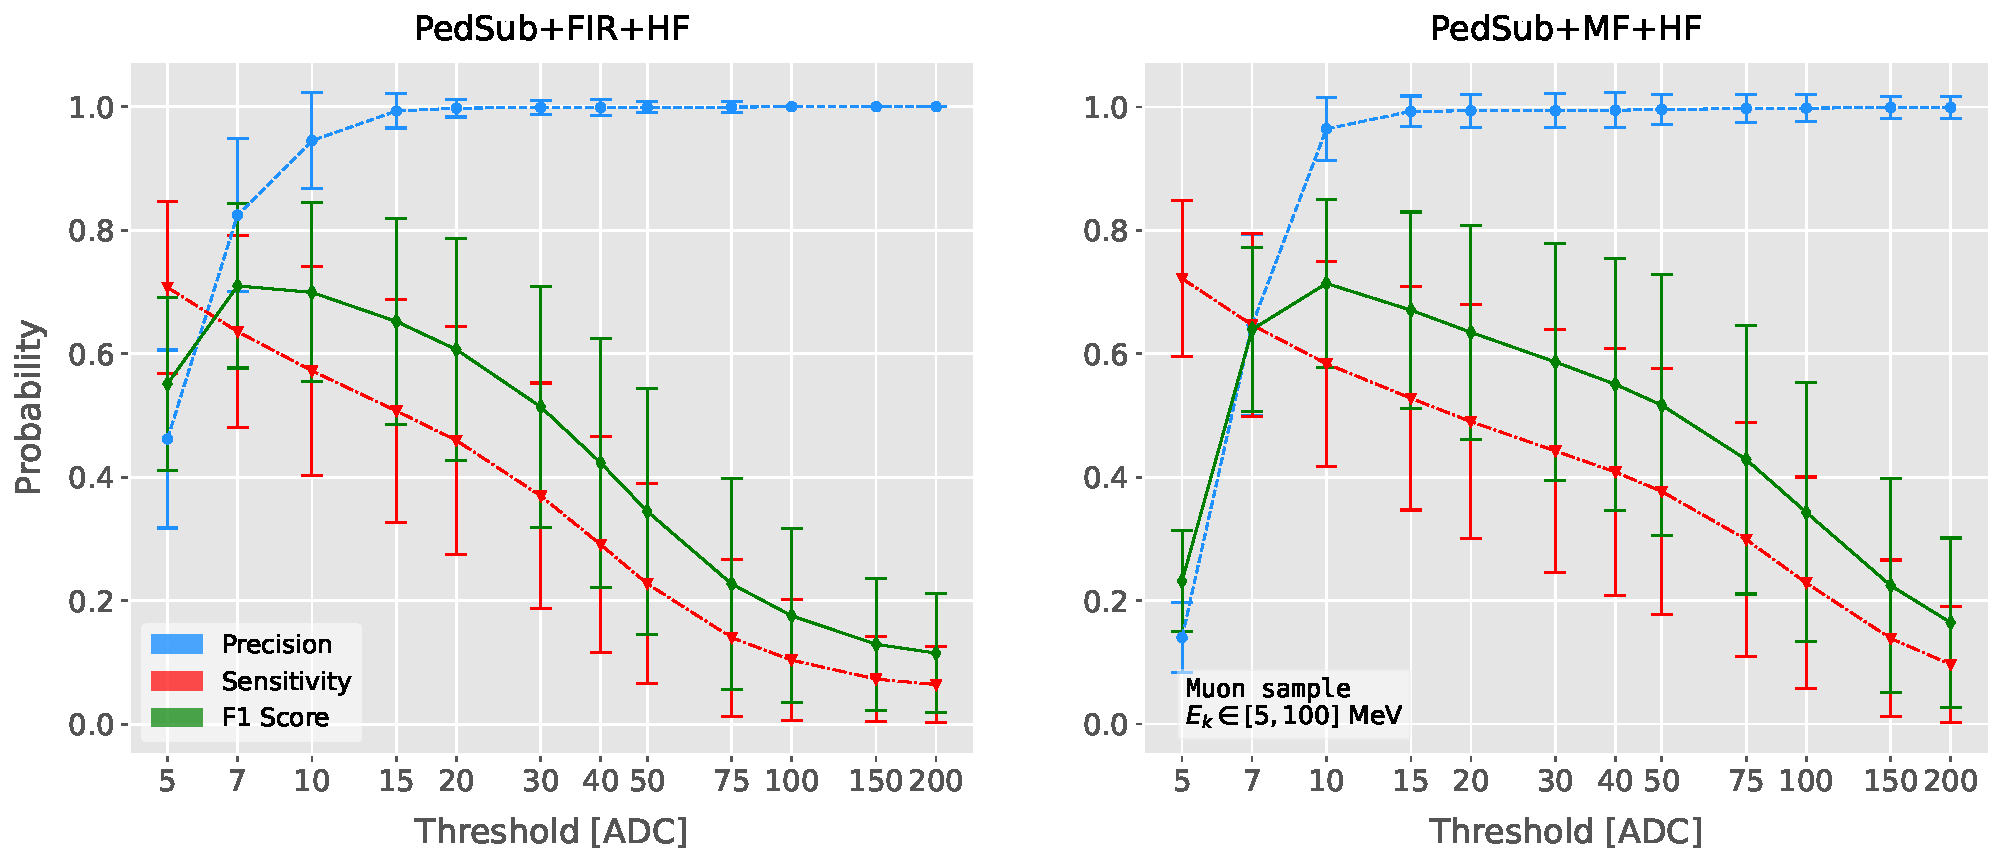
\includegraphics[width=.99\linewidth]{Images/Matched_Filter/hit_study_muon_scores_indct}
	\caption[Dependence of the precision, sensitivity, and $F_{1}$ scores on the threshold values used in the hit finder for the FIR and matched filters.]{Dependence of the precision (blue), sensitivity (red), and $F_{1}$ (green) scores on the threshold values used in the hit finder, for the FIR (left panel) and matched filter (right panel) cases. The results were obtained after matching the hits to the true hits in the case of the isotropic muon sample with kinetic energy in the range $5$ to $100 \ \mathrm{MeV}$, taking only into account the induction plane channels. The points represent the mean value while the error bars indicate one standard deviation around that mean value.}
	\label{fig:threshold_opt}
\end{figure}

The contents of the confusion matrix allow us to compute other derived scores to assess the performance of our classification. In this study, I make use of three of these metrics, namely the precision or positive predictive value:
\begin{equation}
	\mathrm{PPV} = \frac{\mathrm{TP}}{\mathrm{TP} + \mathrm{FP}},
\end{equation}
the sensitivity or true positive rate:
\begin{equation}
	\mathrm{TPR} = \frac{\mathrm{TP}}{\mathrm{TP} + \mathrm{FN}},
\end{equation}
and the $F_{1}$ score \cite{Taha2015}:
\begin{equation}
	F_{1} = \frac{\mathrm{2 TP}}{2\mathrm{TP} + \mathrm{FP} + \mathrm{FN}},
\end{equation}
which is the harmonic mean of the precision and the sensitivity.

For this specific case I am not going to make use of the true negative category, as its definition in this context can be ambiguous because one does not have clear instances in the classification process. This way, I only count the number of true positives as the total amount of hits I can match between true and raw populations, the number of false negatives will be the number of missing true hits, and the false positives the number of hits which do not match any true hit.

In Fig. \ref{fig:threshold_opt} I show the precision (blue), sensitivity (red) and $F_{1}$-score (green) I obtain as a function of the threshold used in the hit finder for the muon sample. Because the matched filters are only applied to induction channels, I consider exclusively the hits coming from the U and V planes. The panel on the left corresponds to the results I get when running the hit finder on the FIR filtered waveforms, whereas the right panel contains the scores for the matched filter case. The points are centered at the threshold value used and represent the mean value obtained for each score using all the generated events, while the error bars indicate one standard deviation around the mean value.

One can see that the precision for the matched filter case is lower when the thresholds are very low, as the noise baseline is slightly amplified, but then rises to high values quicker than for the FIR case. The other difference one can spot is that the sensitivity in the FIR case starts dropping faster at around the same threshold values where the precision stabilises around $1$, while in contrast for the matched filter this rapid decrease starts at higher threshold values. A similar scan for the same thresholds was performed for the electron sample in the same energy range, yielding similar results.

\begin{figure}[t]
	\begin{subfigure}{0.5\textwidth}
		\centering
		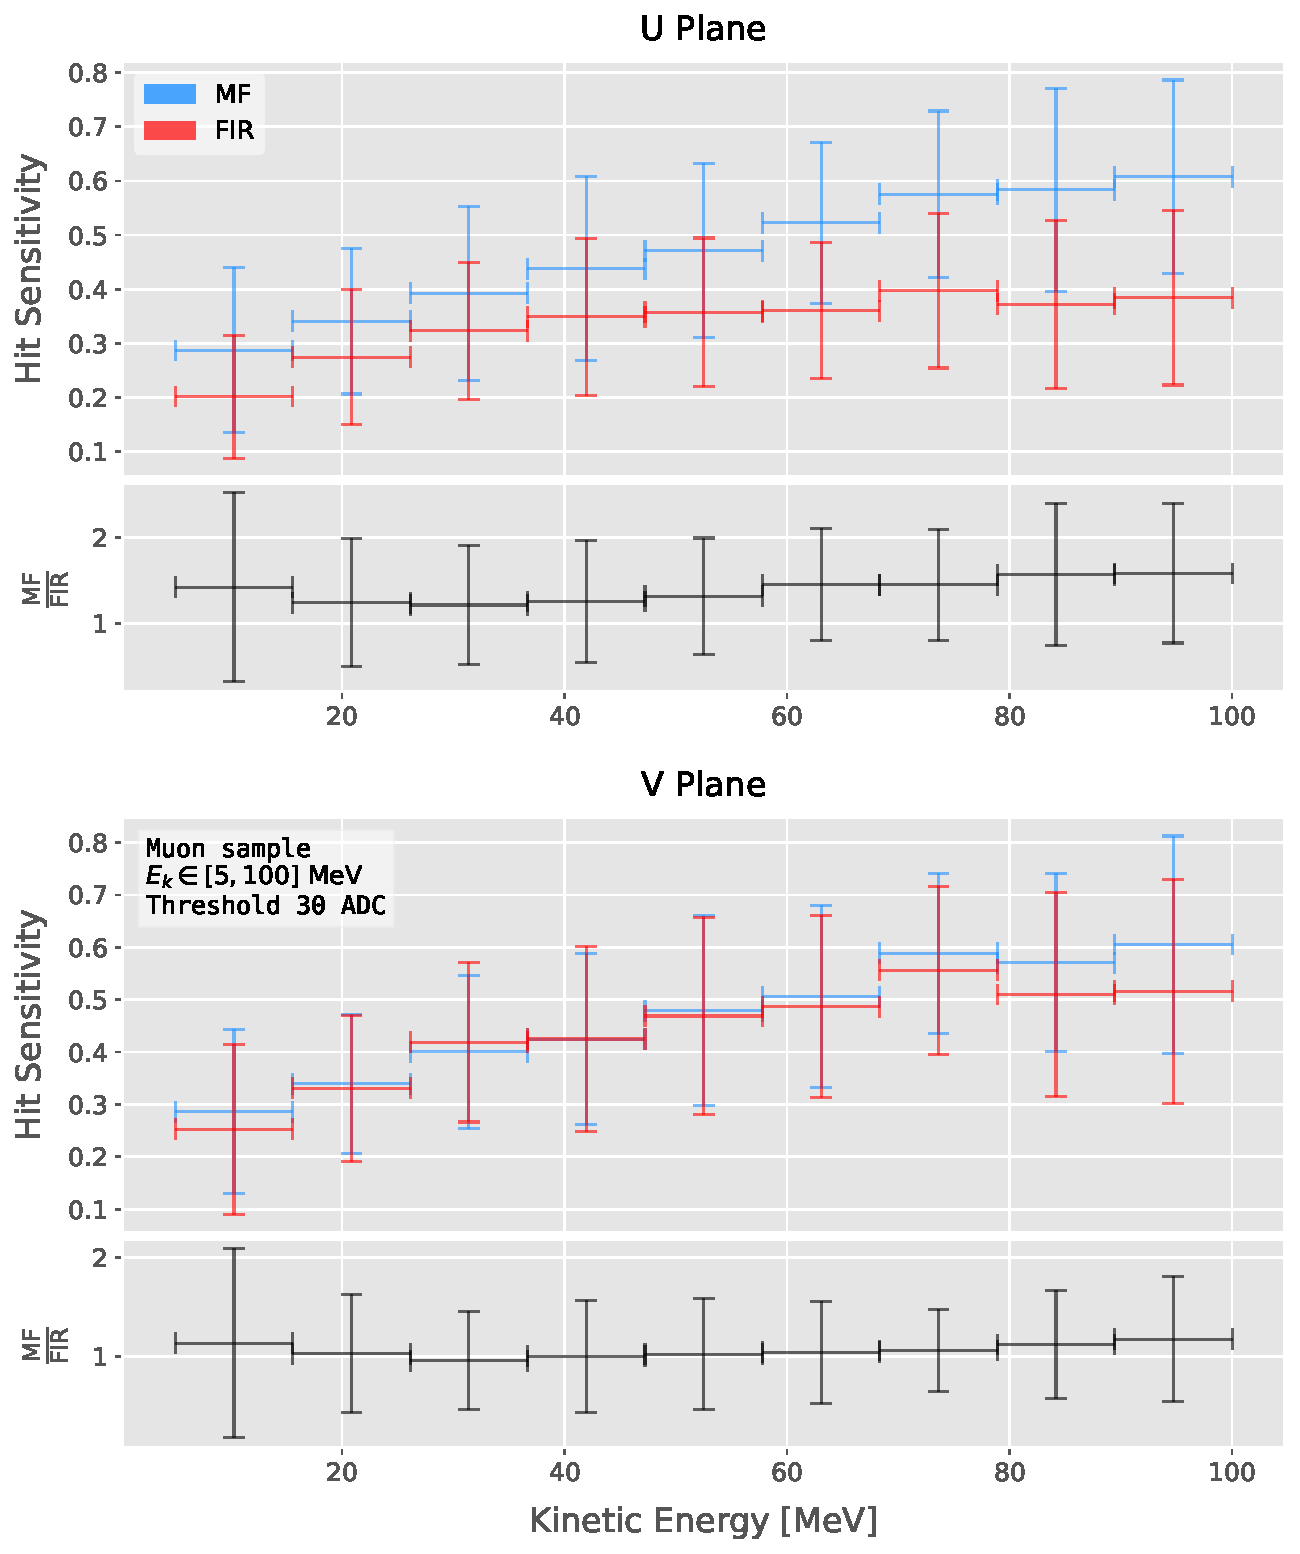
\includegraphics[width=.99\linewidth]{Images/Matched_Filter/hit_study_muon_sensitivity_30}
	\end{subfigure}
	\begin{subfigure}{0.5\textwidth}
		\centering
		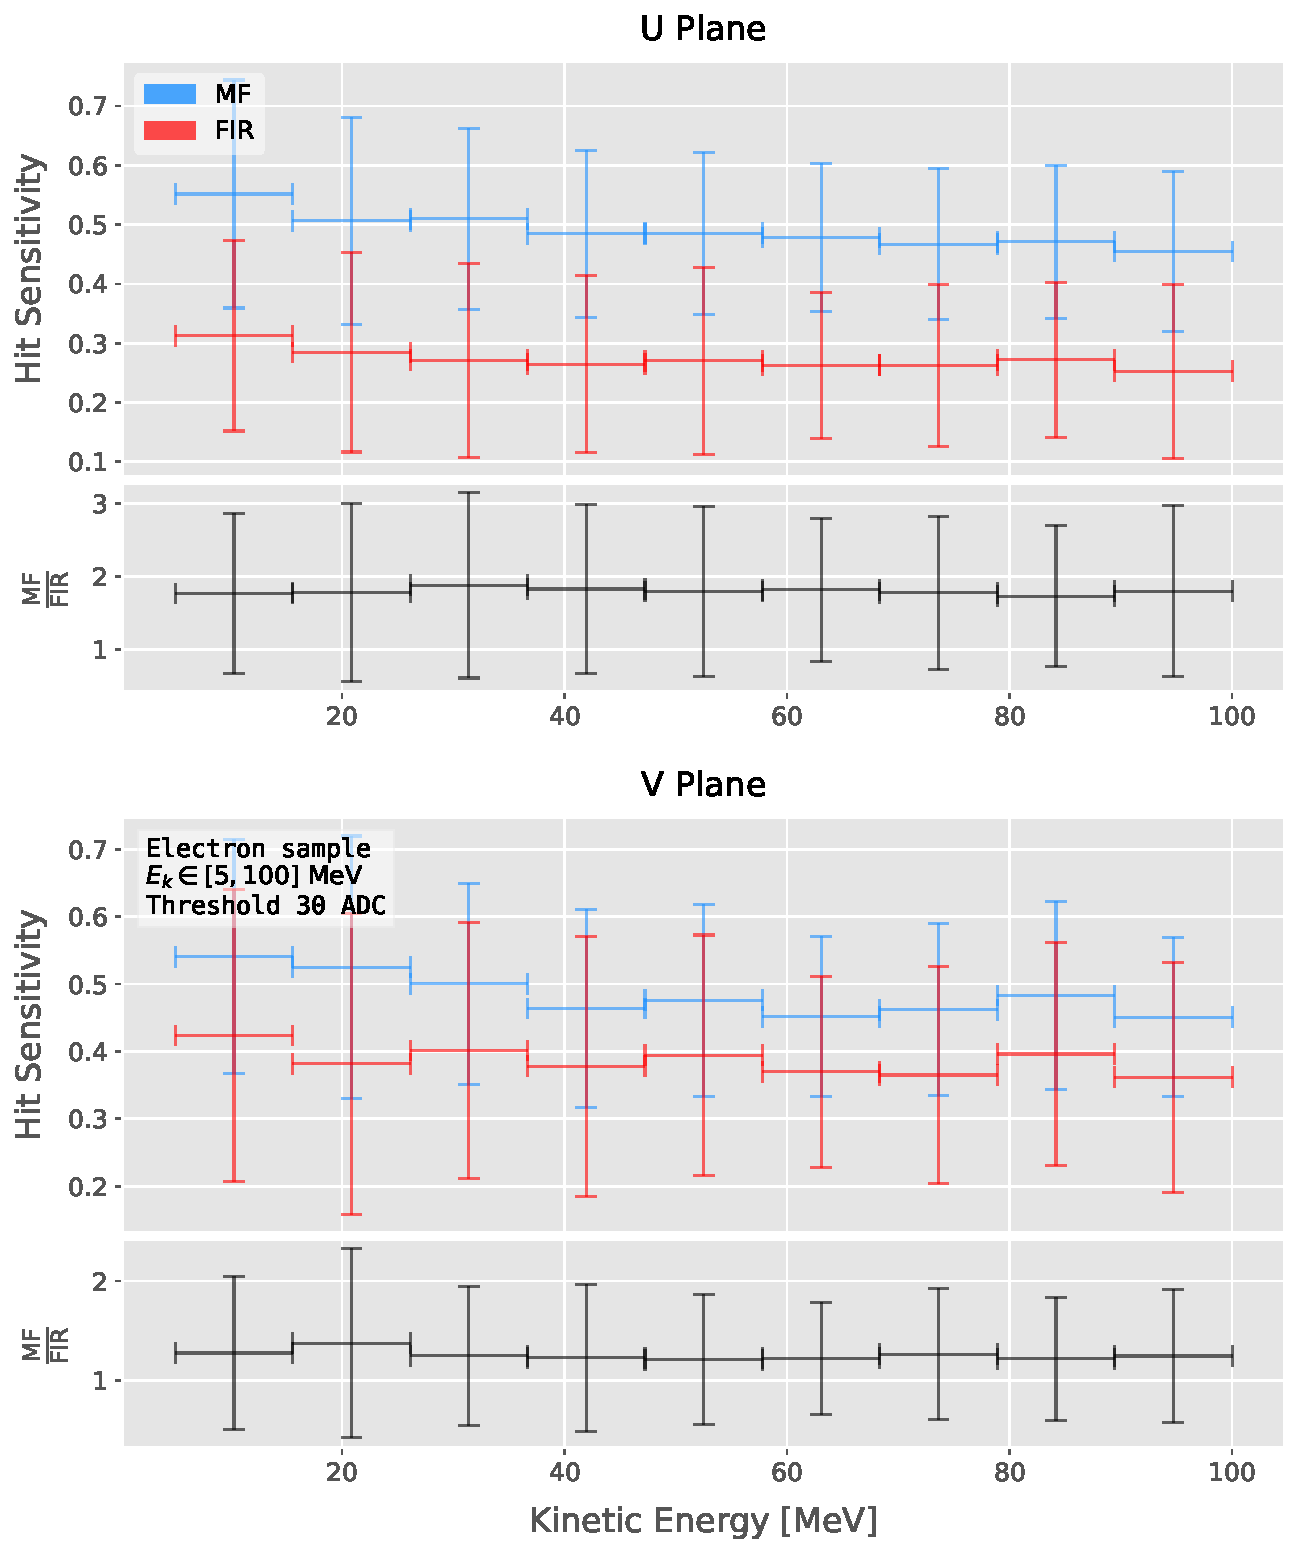
\includegraphics[width=.99\linewidth]{Images/Matched_Filter/hit_study_electron_sensitivity_30}
	\end{subfigure}
	\caption[Dependence of the averaged hit sensitivity on the kinetic energy of the events for the matched filter and standard hits, for the case of the muon and electron samples.]{Dependence of the averaged hit sensitivity on the kinetic energy of the events for the matched filter (blue) and standard (red) hits, for the case of the muon (left panel) and electron (right panel) samples, separated between U (top plots) and V (bottom plots) induction wire planes. The top subplots contain the hit sensitivities for the two hit finder alternatives, while the bottom subplots show the ratio between the two. The horizontal lines sit at the mean value and represent the size of the energy bins, while the vertical error bars indicate one standard deviation around that mean value.}
	\label{fig:sensitivity_energy}
\end{figure}

In Fig. \ref{fig:sensitivity_energy} I show the average hit sensitivity versus the kinetic energy of the events, both for the matched filter hits (blue) and the standard hits (red). The left panel corresponds to the muon sample, whereas the one on the right corresponds to the electron sample, both with kinetic energies between $5$ and $100 \ \mathrm{MeV}$. In each panel, the top plot corresponds to hits in the U plane, while the bottom plot contains the same information for the V plane. Each plot contains two subplots, the one on the top shows the hit sensitivity values for the matched filter and standard hits separate, while the bottom subplot depicts the ratio between the matched filter and standard sensitivities. The horizontal lines are placed at the mean value obtained in the fit and represent the width of the $E_{k}$ bins used, while the vertical error bars indicate one standard deviation around that mean. In both cases, the threshold used was $30 \ \mathrm{ADC}$, as I require the precision to be higher than $0.99$ for both matched filter and standard cases.

\begin{figure}[t]
	\centering
	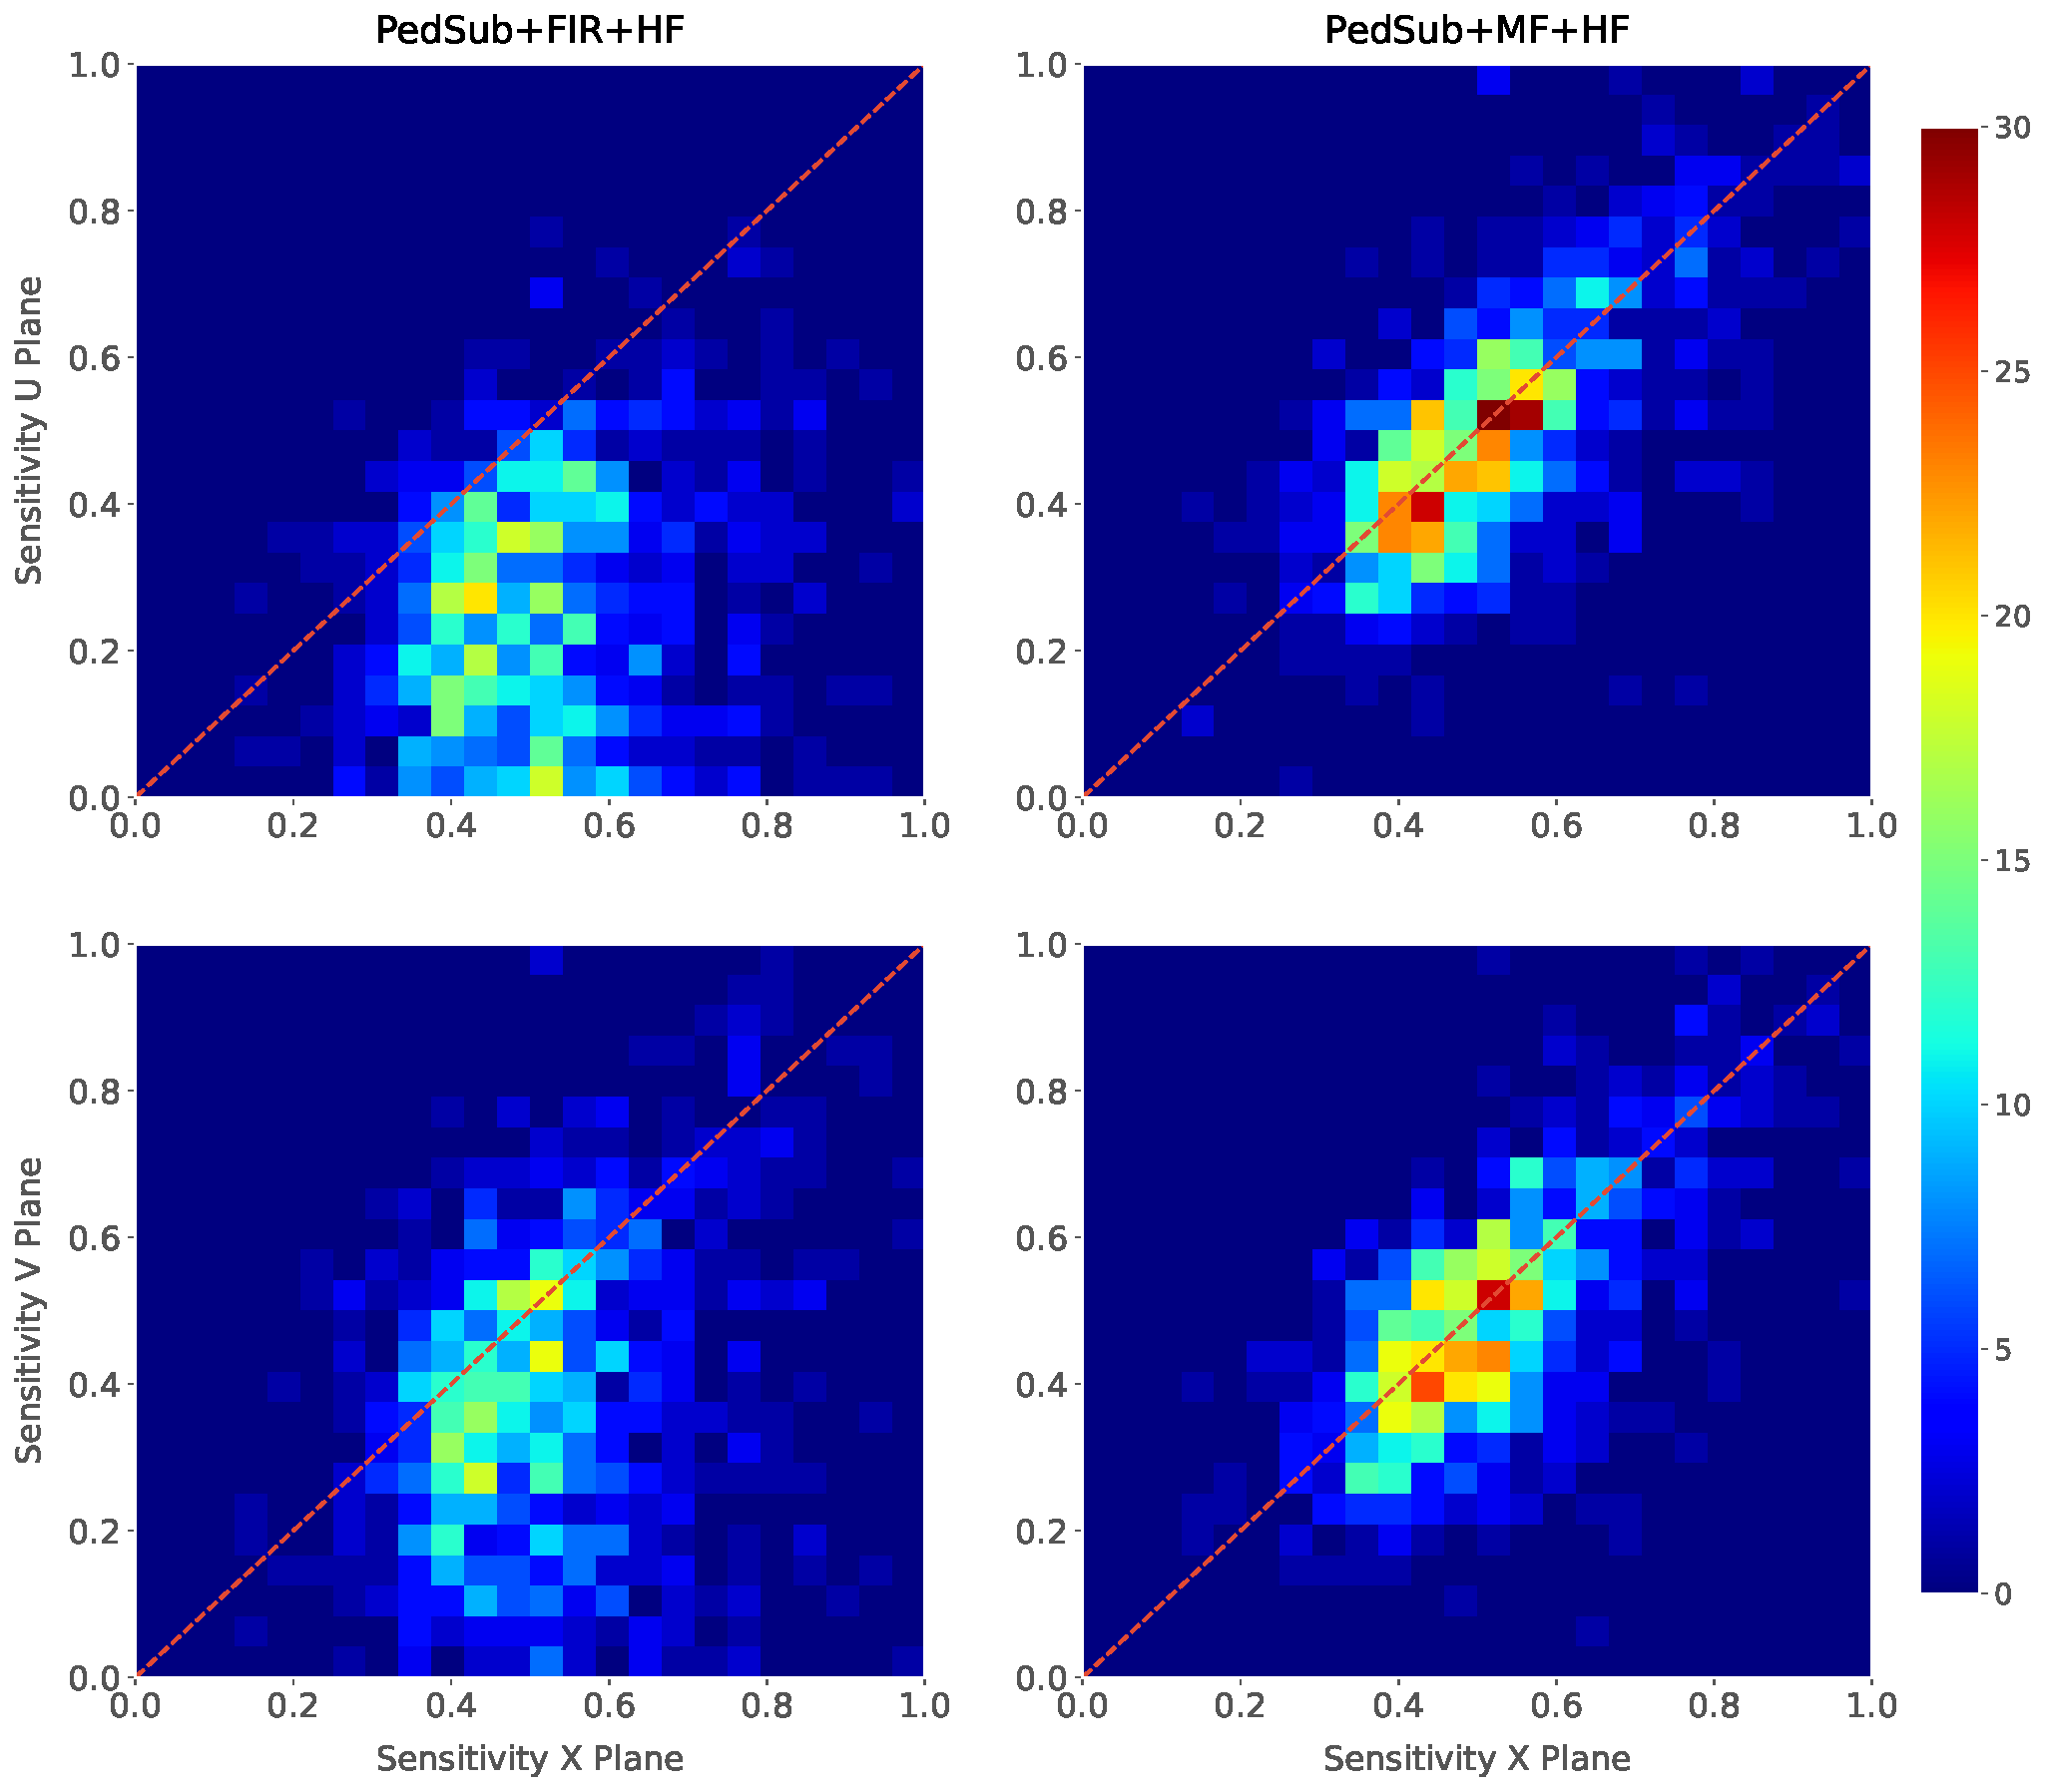
\includegraphics[width=.99\linewidth]{Images/Matched_Filter/hit_study_electron_concurrence}
	\caption[Distributions of the hit sensitivity in the U and V planes versus the sensitivity in the X plane for the standard hits and the matched filter hits in the electron sample.]{Distributions of the hit sensitivity in the U (top panels) and V (bottom panels) planes versus the hit sensitivity in the X plane, both for the standard hits (left panels) and the matched filter hits (right panels), in the case of the electron sample and a threshold of $30 \ \mathrm{ADC}$.}
	\label{fig:electron_concurrence}
\end{figure}

In general, the improvements are better for the U than for the V plane. While for the U channels I achieve a mean improvement of $50\%$ and $80\%$ for muons and electrons, respectively, the improvement in the V plane is stalled at $10\%$ and $25\%$. Nevertheless, looking at the sensitivities for the matched filter hits in both planes, one can see these have similar mean values for each energy bin. On the other hand, for the standard hits the sensitivity remains higher for the V plane. This way, it looks there is a less significant gain because the hit sensitivity was already high.

Another interesting observation is the different behaviors for muons and electrons. While hit sensitivity for muons grows significantly with energy, in the case of electrons it slightly decreases the higher the kinetic energy of the event is. However, when it comes to the improvement on the sensitivities, this remains almost constant in all cases.

\begin{figure}[t]
	\centering
	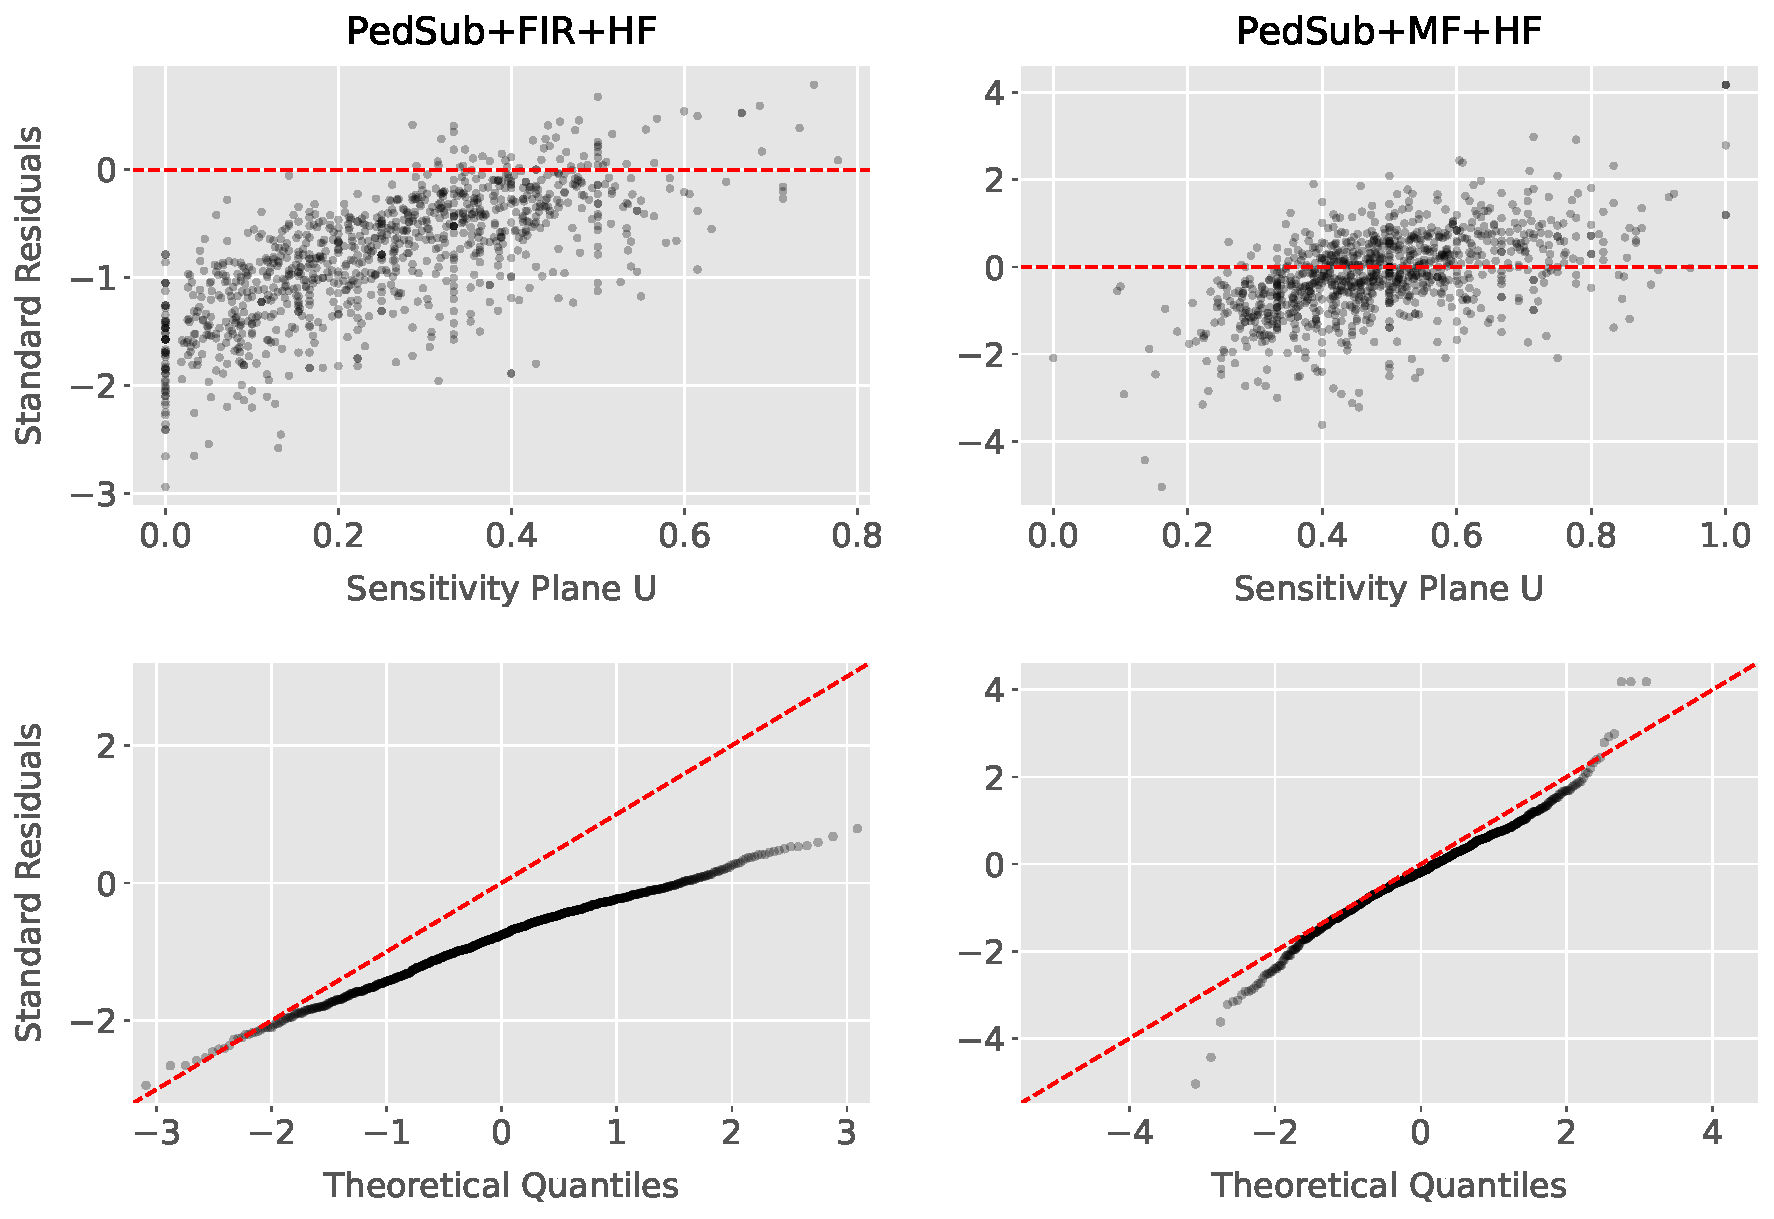
\includegraphics[width=.99\linewidth]{Images/Matched_Filter/hit_study_electron_residuals}
	\caption[Standard residuals and quantile-quantile plots for the hit sensitivity of the X and U planes.]{Top panels: standard residual plots of the hit sensitivities between the X and U planes. Bottom panels: quantile-quantile plots of the hit sensitivity standard residuals between the X and U planes. In all cases, the left panel corresponds to the standard hits while the right panel represents the matched filter case, all from the electron sample with a $30 \ \mathrm{ADC}$ threshold.}
	\label{fig:electron_residuals}
\end{figure}

Furthermore, we can look at how the concurrence of hits between the different wire planes has changed. For any given event, I expect to have a similar number of hits in the three planes. As the ionisation electrons need to cross the U and V planes prior to reach the collection plane X, they will induce current in those wire planes. A way to check the concurrence of hits across planes is comparing the hit sensitivities in the different planes for each individual event. Although the sensitivities will not be exactly equal across planes, ideally they should be normally distributed around the diagonal.

Figure \ref{fig:electron_concurrence} shows the hit sensitivity in the U (top panels) and V (bottom panels) planes versus the hit sensitivity in the X plane, for the case of the standard hits (left panels) and the matched filter hits (right panels). All plots were generated for the electron sample and a threshold of $30 \ \mathrm{ADC}$. From these, one can see a clear trend. The standard hit finder chain produces hit sensitivities in the induction planes that are systematically lower than the sensitivity in the X plane, i.e. most of the points sit below the diagonal (red dashed line). In contrast, when the matched filters are applied, the majority of the events are distributed around the diagonal. This points out that the concurrence of hits across planes has improved.

To exemplify the improvement I obtain, I take the residuals of the hit sensitivities for the X and U planes. Assuming the diagonal hypothesis, i.e. given a dataset of the form $(x, y)$ for any $x$ I take the predicted $y$ value to be equal to the value of $x$, I can compute the standard residuals for the hit sensitivities in U given the sensitivities for X. In Fig. \ref{fig:electron_residuals} (top panels) I show these standard residuals against the corresponding values of the hit sensitivity in the U plane, for the electron sample with kinetic energy between $5$ and $100 \ \mathrm{MeV}$. Comparing the scatter points in the case of the standard hits (left panel) and the matched filter hits (right panel), it can be seen that the residuals for the standard hit finder follow a certain pattern and their mean deviates from $0$.

To see clearly if the residuals are normally distributed, in Fig. \ref{fig:electron_residuals} (bottom panels) I plot the corresponding quantile-quantile plot for both the standard (left panel) and matched filter (right panel) residuals. One can clearly see that the points for the standard hit finder case follow a strongly non-linear pattern, suggesting that the residuals do not follow a normal distribution. In contrast, for the matched filter hits the points conform to a roughly linear path, implying that in this case the normality condition is fulfilled.

All these results hint at the fact that the concurrence of hits across the wire planes can be strengthened by applying the matched filters.

\begin{figure}[t]
    \centering
    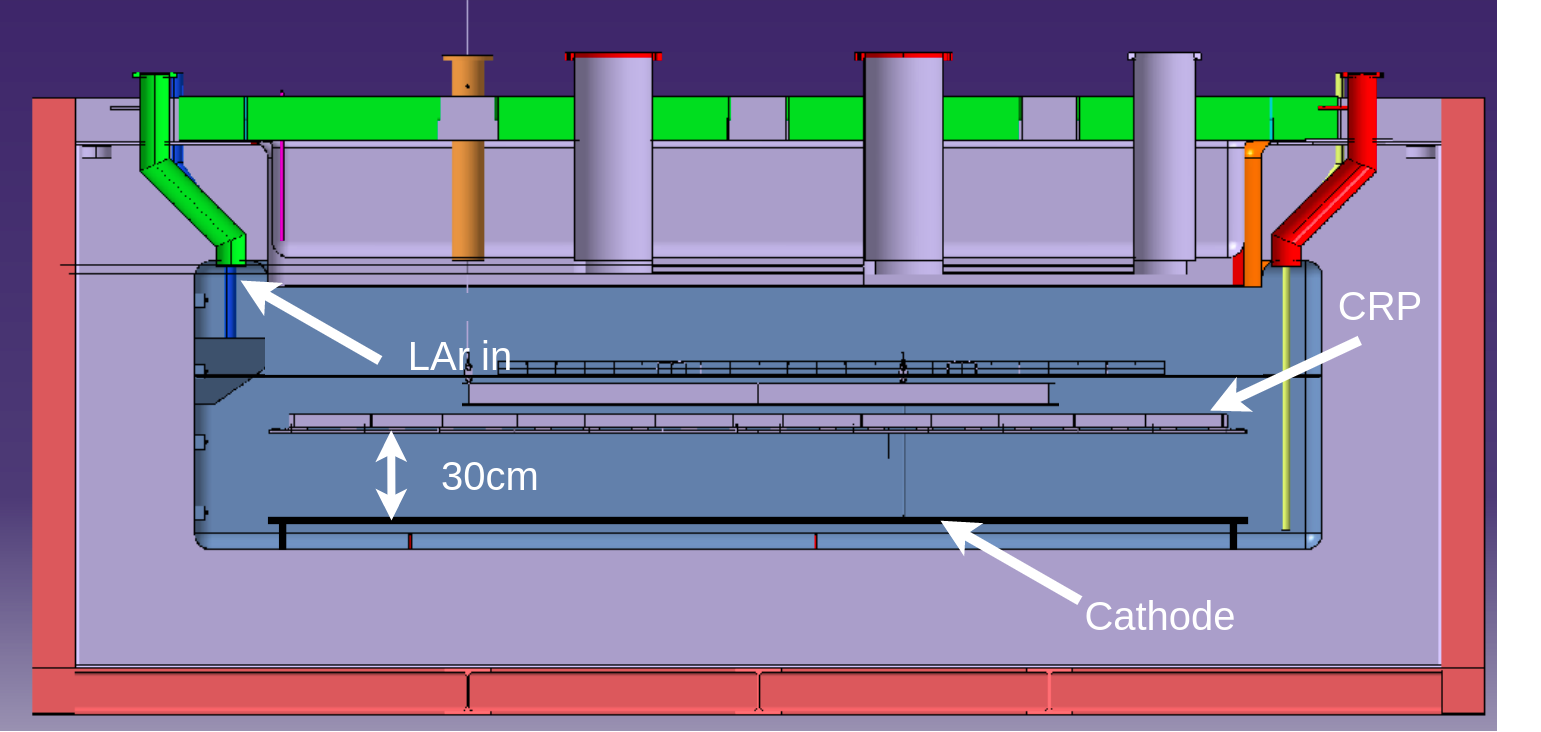
\includegraphics[scale = 0.2]{Images/Matched_Filter/VD_Coldbox_Diagram.png}
    \caption{Schematic diagram of the vertical drift ColdBox setup at CERN.}
    \label{fig:vdcoldbox}
\end{figure}

\section{VD ColdBox data taking}
\label{sec:matched_filter_vdcoldbox}

\begin{figure}[t]
    \centering
    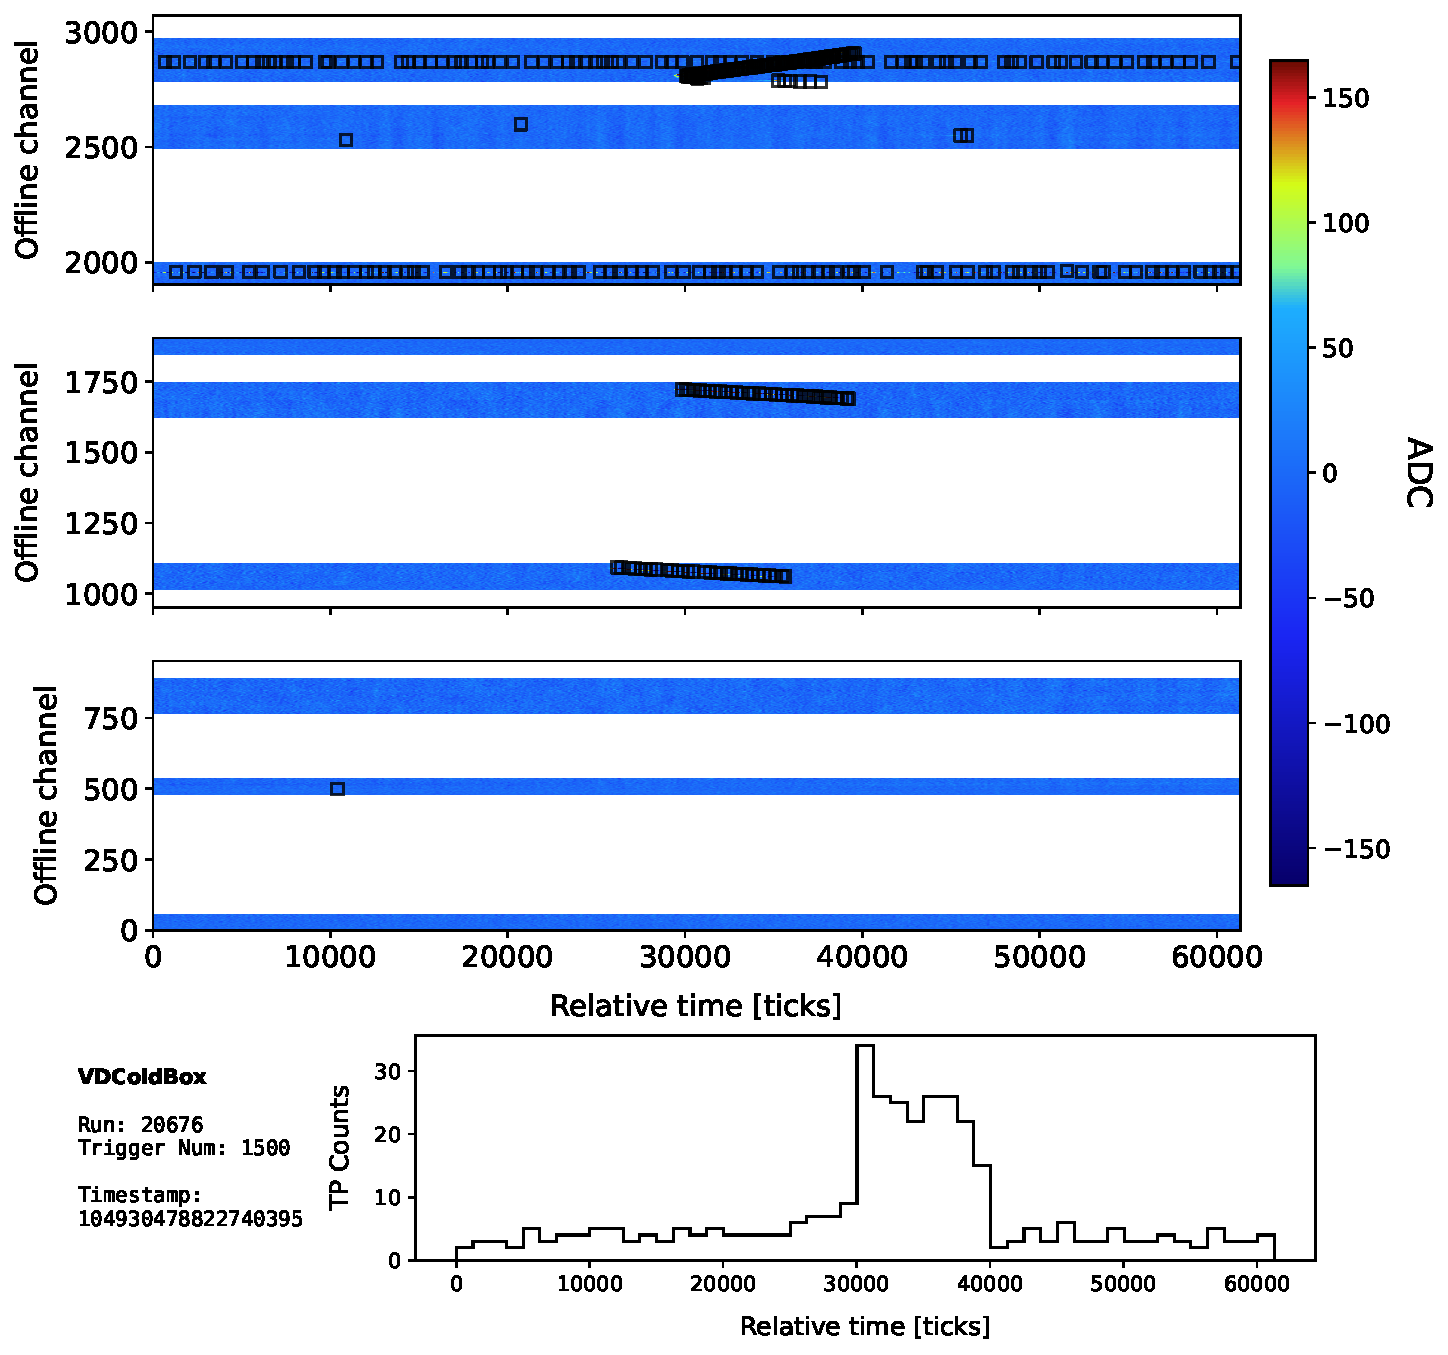
\includegraphics[scale = 0.5]{Images/Matched_Filter/TRDisplay_np02_coldbox_run020676_0001.pdf}
    \caption[Event display of the data taken with the matched filter and HMA trigger at the VD ColdBox.]{Event display of the data taken with the matched filter and HMA trigger at the VD ColdBox. The display shows the data from 3 ADC links for the full trigger window, with the black squares representing the produced TPs. The bottom panel represents the TP counts as a function of time in the trigger window.}
    \label{fig:example_hma_evd}
\end{figure}

Between February and April 2023 the vertical drift (VD) ColdBox setup at CERN, shown in Fig. \ref{fig:vdcoldbox}, was recommissioned for cold electronics testing with CRP5. That provided an opportunity for testing the firmware TP generation in a real LArTPC. However, during the two run periods new software-related complications that were not observed in previous running conditions arose.

These prevented us from taking data with the whole system. As a palliative measure, new configurations were developed that allowed to run with TP generation enabled for a subset of the ADC links. With these workarounds, we managed to run with up to three out of twelve ADC links and the horizontal muon trigger algorithm (HMA).

\begin{figure}[t]
    \centering
    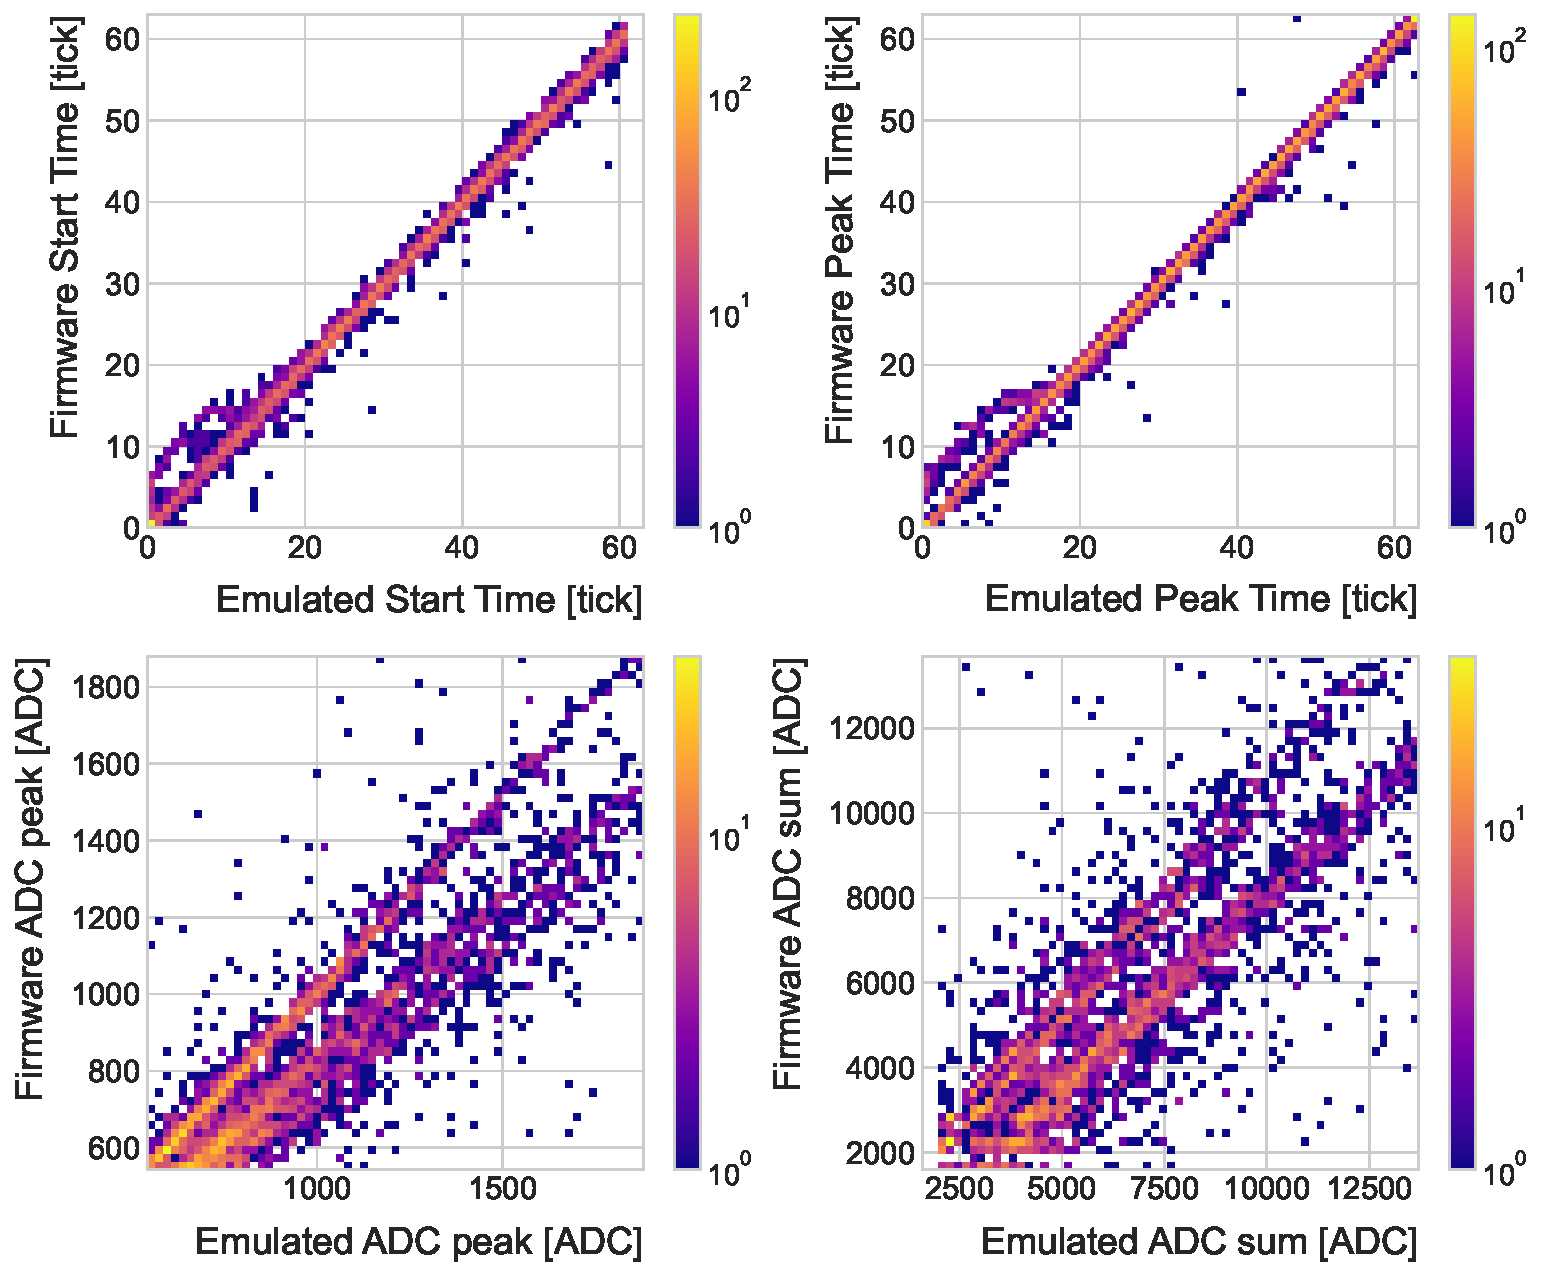
\includegraphics[scale = 0.5]{Images/Matched_Filter/np02_coldbox_tp_comp.pdf}
    \caption[Comparison between firmware-produced and simulated TP quantities for a matched filter run at the VD ColdBox.]{Comparison between firmware-produced and simulated TP quantities for a matched filter run at the VD ColdBox.}
    \label{fig:vdcoldbox_tp_comp}
\end{figure}

Additionally, an alternative firmware version was prepared featuring the matched filter coefficients optimised for the induction plane hit finding. The version of the filter we used for the data taking is slightly different from the one of the previous studies, as in this case we needed to apply the same filter coefficients to all channels irrespective of the readout plane they come from. With this, we also managed to run with three ADC links and the HMA trigger. Figure \ref{fig:example_hma_evd} shows an example event display from the longest run we recorded with the matched filter firmware.

We used the recorded data, together with our standalone TPG simulation tool, to perform comparisons between the firmware and simulated TPs. One such comparison for a matched filter run can be seen in Fig. \ref{fig:vdcoldbox_tp_comp}. The agreement achieved is within the expectation, from what we have seen in previous samples.

All the studies presented demonstrate the robustness of the matched filter approach to form TPs. I have used both ProtoDUNE-SP data and MC samples to assess its impact on the S/N and TP production of the induction channels. Additionally, I have shown that it is possible to run with it in a real detector environment, after the tests at the VD ColdBox setup.